\documentclass[aps,prb,twocolumn,superscriptaddress,amsmath]{revtex4-2}
% \documentclass[aps,prb,twocolumn,superscriptaddress,amsmath]{standalone}

\usepackage{pgfplots}
\usetikzlibrary{arrows.meta}

\pgfplotsset{compat=newest,
   width=7cm,
   height=5cm,
   scale only axis=true,
   max space between ticks=25pt,
   try min ticks=5,
   every axis/.style={
        axis line style={thick,->,>=latex, shorten >=-.4cm}
    },
    every axis plot/.append style={thick},
    tick style={black, thick}
}
\tikzset{
    semithick/.style={line width=0.8pt},
}
\usepgfplotslibrary{groupplots}
\usepgfplotslibrary{dateplot}

\begin{document}
%
\section{Test section}

% Here is some sample text to fill the column. 

\begin{figure}[h]
    \centering
    % This file was created with tikzplotlib v0.10.1.post13.
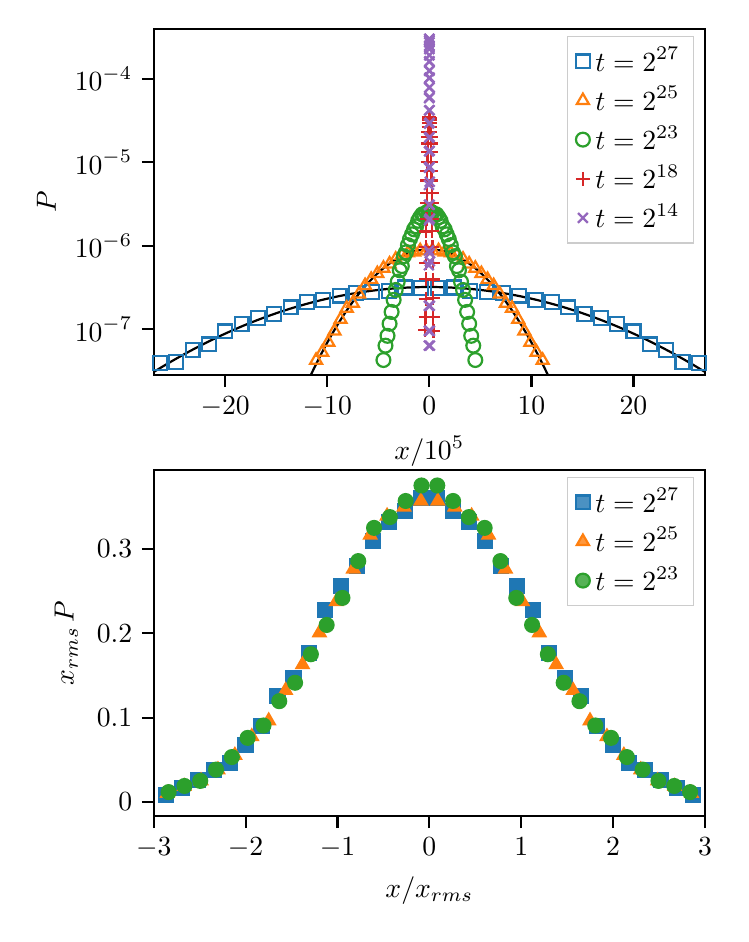
\begin{tikzpicture}

\definecolor{crimson2143940}{RGB}{214,39,40}
\definecolor{darkgrey176}{RGB}{176,176,176}
\definecolor{darkorange25512714}{RGB}{255,127,14}
\definecolor{forestgreen4416044}{RGB}{44,160,44}
\definecolor{lightgrey204}{RGB}{204,204,204}
\definecolor{mediumpurple148103189}{RGB}{148,103,189}
\definecolor{orchid227119194}{RGB}{227,119,194}
\definecolor{sienna1408675}{RGB}{140,86,75}
\definecolor{steelblue31119180}{RGB}{31,119,180}

\begin{groupplot}[group style={group size=1 by 2, vertical sep=1.2cm}, height=4.4cm, width=7cm]
\nextgroupplot[
legend cell align={left},
legend style={fill opacity=0.8, draw opacity=1, text opacity=1, draw=lightgrey204},
log basis y={10},
tick align=outside,
tick pos=left,
x grid style={darkgrey176},
xlabel={\(\displaystyle x/10^5\)},
xmin=-27, xmax=27,
xtick style={color=black},
y grid style={darkgrey176},
ylabel={\(\displaystyle  P \)},
ymin=2.8e-08, ymax=0.0004,
ymode=log,
ytick style={color=black},
ytick={1e-09,1e-08,1e-07,1e-06,1e-05,0.0001,0.001,0.01},
yticklabels={
  \(\displaystyle {10^{-9}}\),
  \(\displaystyle {10^{-8}}\),
  \(\displaystyle {10^{-7}}\),
  \(\displaystyle {10^{-6}}\),
  \(\displaystyle {10^{-5}}\),
  \(\displaystyle {10^{-4}}\),
  \(\displaystyle {10^{-3}}\),
  \(\displaystyle {10^{-2}}\)
}
]
\addplot [semithick, black, forget plot]
table {%
-30 1.77140129867429e-08
-29.9399399399399 1.79202612585694e-08
-29.8798798798799 1.81284903702559e-08
-29.8198198198198 1.83387136215314e-08
-29.7597597597598 1.85509443269235e-08
-29.6996996996997 1.87651958146873e-08
-29.6396396396396 1.89814814257204e-08
-29.5795795795796 1.91998145124637e-08
-29.5195195195195 1.94202084377885e-08
-29.4594594594595 1.96426765738695e-08
-29.3993993993994 1.98672323010433e-08
-29.3393393393393 2.00938890066533e-08
-29.2792792792793 2.03226600838809e-08
-29.2192192192192 2.05535589305617e-08
-29.1591591591592 2.07865989479887e-08
-29.0990990990991 2.10217935397004e-08
-29.039039039039 2.12591561102561e-08
-28.978978978979 2.14987000639963e-08
-28.9189189189189 2.17404388037894e-08
-28.8588588588589 2.19843857297646e-08
-28.7987987987988 2.22305542380304e-08
-28.7387387387387 2.24789577193799e-08
-28.6786786786787 2.27296095579813e-08
-28.6186186186186 2.29825231300554e-08
-28.5585585585586 2.32377118025387e-08
-28.4984984984985 2.34951889317331e-08
-28.4384384384384 2.3754967861941e-08
-28.3783783783784 2.4017061924088e-08
-28.3183183183183 2.42814844343306e-08
-28.2582582582583 2.45482486926512e-08
-28.1981981981982 2.48173679814389e-08
-28.1381381381381 2.5088855564057e-08
-28.0780780780781 2.5362724683397e-08
-28.018018018018 2.56389885604192e-08
-27.957957957958 2.59176603926794e-08
-27.8978978978979 2.61987533528434e-08
-27.8378378378378 2.6482280587187e-08
-27.7777777777778 2.67682552140833e-08
-27.7177177177177 2.70566903224772e-08
-27.6576576576577 2.73475989703463e-08
-27.5975975975976 2.76409941831491e-08
-27.5375375375375 2.79368889522602e-08
-27.4774774774775 2.82352962333928e-08
-27.4174174174174 2.85362289450081e-08
-27.3573573573574 2.88396999667126e-08
-27.2972972972973 2.91457221376421e-08
-27.2372372372372 2.94543082548341e-08
-27.1771771771772 2.9765471071587e-08
-27.1171171171171 3.00792232958076e-08
-27.0570570570571 3.03955775883457e-08
-26.996996996997 3.07145465613178e-08
-26.9369369369369 3.10361427764176e-08
-26.8768768768769 3.13603787432151e-08
-26.8168168168168 3.16872669174445e-08
-26.7567567567568 3.20168196992793e-08
-26.6966966966967 3.23490494315971e-08
-26.6366366366366 3.26839683982321e-08
-26.5765765765766 3.30215888222169e-08
-26.5165165165165 3.33619228640128e-08
-26.4564564564565 3.37049826197294e-08
-26.3963963963964 3.40507801193331e-08
-26.3363363363363 3.43993273248447e-08
-26.2762762762763 3.47506361285272e-08
-26.2162162162162 3.51047183510622e-08
-26.1561561561562 3.54615857397164e-08
-26.0960960960961 3.58212499664982e-08
-26.036036036036 3.6183722626304e-08
-25.975975975976 3.65490152350548e-08
-25.9159159159159 3.69171392278228e-08
-25.8558558558559 3.72881059569491e-08
-25.7957957957958 3.76619266901516e-08
-25.7357357357357 3.8038612608624e-08
-25.6756756756757 3.84181748051254e-08
-25.6156156156156 3.88006242820615e-08
-25.5555555555556 3.9185971949557e-08
-25.4954954954955 3.95742286235198e-08
-25.4354354354354 3.99654050236962e-08
-25.3753753753754 4.03595117717189e-08
-25.3153153153153 4.07565593891465e-08
-25.2552552552553 4.11565582954958e-08
-25.1951951951952 4.15595188062661e-08
-25.1351351351351 4.19654511309565e-08
-25.0750750750751 4.23743653710762e-08
-25.015015015015 4.27862715181479e-08
-24.954954954955 4.32011794517039e-08
-24.8948948948949 4.36190989372773e-08
-24.8348348348348 4.40400396243847e-08
-24.7747747747748 4.44640110445053e-08
-24.7147147147147 4.48910226090527e-08
-24.6546546546547 4.53210836073412e-08
-24.5945945945946 4.57542032045476e-08
-24.5345345345345 4.61903904396674e-08
-24.4744744744745 4.66296542234658e-08
-24.4144144144144 4.70720033364248e-08
-24.3543543543544 4.75174464266855e-08
-24.2942942942943 4.79659920079868e-08
-24.2342342342342 4.84176484575989e-08
-24.1741741741742 4.88724240142549e-08
-24.1141141141141 4.93303267760782e-08
-24.0540540540541 4.97913646985062e-08
-23.993993993994 5.02555455922125e-08
-23.9339339339339 5.07228771210255e-08
-23.8738738738739 5.11933667998449e-08
-23.8138138138138 5.16670219925564e-08
-23.7537537537538 5.21438499099446e-08
-23.6936936936937 5.26238576076038e-08
-23.6336336336336 5.31070519838487e-08
-23.5735735735736 5.35934397776232e-08
-23.5135135135135 5.40830275664087e-08
-23.4534534534535 5.45758217641324e-08
-23.3933933933934 5.50718286190758e-08
-23.3333333333333 5.55710542117819e-08
-23.2732732732733 5.60735044529649e-08
-23.2132132132132 5.65791850814194e-08
-23.1531531531532 5.70881016619311e-08
-23.0930930930931 5.76002595831887e-08
-23.033033033033 5.81156640556982e-08
-22.972972972973 5.8634320109698e-08
-22.9129129129129 5.91562325930775e-08
-22.8528528528529 5.96814061692981e-08
-22.7927927927928 6.02098453153163e-08
-22.7327327327327 6.07415543195111e-08
-22.6726726726727 6.12765372796147e-08
-22.6126126126126 6.18147981006467e-08
-22.5525525525526 6.2356340492853e-08
-22.4924924924925 6.29011679696492e-08
-22.4324324324324 6.34492838455686e-08
-22.3723723723724 6.40006912342159e-08
-22.3123123123123 6.45553930462256e-08
-22.2522522522523 6.51133919872276e-08
-22.1921921921922 6.56746905558177e-08
-22.1321321321321 6.62392910415354e-08
-22.0720720720721 6.68071955228485e-08
-22.012012012012 6.73784058651447e-08
-21.951951951952 6.7952923718731e-08
-21.8918918918919 6.85307505168411e-08
-21.8318318318318 6.91118874736507e-08
-21.7717717717718 6.96963355823015e-08
-21.7117117117117 7.0284095612935e-08
-21.6516516516517 7.08751681107343e-08
-21.5915915915916 7.14695533939762e-08
-21.5315315315315 7.20672515520938e-08
-21.4714714714715 7.26682624437486e-08
-21.4114114114114 7.32725856949138e-08
-21.3513513513514 7.3880220696969e-08
-21.2912912912913 7.44911666048054e-08
-21.2312312312312 7.5105422334944e-08
-21.1711711711712 7.57229865636651e-08
-21.1111111111111 7.63438577251504e-08
-21.0510510510511 7.69680340096387e-08
-20.990990990991 7.7595513361594e-08
-20.9309309309309 7.82262934778878e-08
-20.8708708708709 7.88603718059953e-08
-20.8108108108108 7.94977455422057e-08
-20.7507507507508 8.01384116298471e-08
-20.6906906906907 8.07823667575276e-08
-20.6306306306306 8.14296073573902e-08
-20.5705705705706 8.2080129603385e-08
-20.5105105105105 8.27339294095565e-08
-20.4504504504505 8.33910024283484e-08
-20.3903903903904 8.40513440489244e-08
-20.3303303303303 8.47149493955073e-08
-20.2702702702703 8.53818133257348e-08
-20.2102102102102 8.60519304290343e-08
-20.1501501501502 8.67252950250151e-08
-20.0900900900901 8.74019011618802e-08
-20.03003003003 8.80817426148572e-08
-19.96996996997 8.8764812884648e-08
-19.9099099099099 8.94511051958992e-08
-19.8498498498498 9.01406124956924e-08
-19.7897897897898 9.08333274520553e-08
-19.7297297297297 9.15292424524933e-08
-19.6696696696697 9.22283496025432e-08
-19.6096096096096 9.29306407243482e-08
-19.5495495495495 9.36361073552548e-08
-19.4894894894895 9.43447407464331e-08
-19.4294294294294 9.50565318615183e-08
-19.3693693693694 9.5771471375277e-08
-19.3093093093093 9.64895496722965e-08
-19.2492492492492 9.72107568456973e-08
-19.1891891891892 9.79350826958708e-08
-19.1291291291291 9.86625167292415e-08
-19.0690690690691 9.93930481570537e-08
-19.009009009009 1.00126665894184e-07
-18.9489489489489 1.00863358557978e-07
-18.8888888888889 1.01603114467118e-07
-18.8288288288288 1.0234592164051e-07
-18.7687687687688 1.030917677962e-07
-18.7087087087087 1.03840640350323e-07
-18.6486486486486 1.04592526416071e-07
-18.5885885885886 1.05347412802693e-07
-18.5285285285285 1.06105286014524e-07
-18.4684684684685 1.0686613225004e-07
-18.4084084084084 1.07629937400943e-07
-18.3483483483483 1.08396687051275e-07
-18.2882882882883 1.09166366476564e-07
-18.2282282282282 1.09938960642993e-07
-18.1681681681682 1.10714454206605e-07
-18.1081081081081 1.1149283151254e-07
-18.048048048048 1.12274076594297e-07
-17.987987987988 1.13058173173027e-07
-17.9279279279279 1.13845104656867e-07
-17.8678678678679 1.14634854140293e-07
-17.8078078078078 1.15427404403513e-07
-17.7477477477477 1.16222737911892e-07
-17.6876876876877 1.17020836815406e-07
-17.6276276276276 1.1782168294813e-07
-17.5675675675676 1.18625257827764e-07
-17.5075075075075 1.19431542655182e-07
-17.4474474474474 1.20240518314031e-07
-17.3873873873874 1.21052165370346e-07
-17.3273273273273 1.21866464072212e-07
-17.2672672672673 1.22683394349458e-07
-17.2072072072072 1.23502935813381e-07
-17.1471471471471 1.24325067756512e-07
-17.0870870870871 1.25149769152414e-07
-17.027027027027 1.25977018655515e-07
-16.966966966967 1.2680679460098e-07
-16.9069069069069 1.27639075004617e-07
-16.8468468468468 1.28473837562817e-07
-16.7867867867868 1.29311059652542e-07
-16.7267267267267 1.30150718331332e-07
-16.6666666666667 1.30992790337368e-07
-16.6066066066066 1.31837252089558e-07
-16.5465465465465 1.32684079687667e-07
-16.4864864864865 1.3353324891249e-07
-16.4264264264264 1.3438473522605e-07
-16.3663663663664 1.35238513771849e-07
-16.3063063063063 1.36094559375145e-07
-16.2462462462462 1.36952846543277e-07
-16.1861861861862 1.37813349466025e-07
-16.1261261261261 1.38676042016011e-07
-16.0660660660661 1.39540897749133e-07
-16.006006006006 1.40407889905052e-07
-15.9459459459459 1.41276991407704e-07
-15.8858858858859 1.4214817486586e-07
-15.8258258258258 1.43021412573729e-07
-15.7657657657658 1.43896676511592e-07
-15.7057057057057 1.44773938346481e-07
-15.6456456456456 1.45653169432905e-07
-15.5855855855856 1.46534340813605e-07
-15.5255255255255 1.47417423220358e-07
-15.4654654654655 1.48302387074822e-07
-15.4054054054054 1.49189202489415e-07
-15.3453453453453 1.50077839268243e-07
-15.2852852852853 1.50968266908069e-07
-15.2252252252252 1.51860454599318e-07
-15.1651651651652 1.52754371227125e-07
-15.1051051051051 1.53649985372434e-07
-15.045045045045 1.54547265313123e-07
-14.984984984985 1.55446179025183e-07
-14.9249249249249 1.56346694183938e-07
-14.8648648648649 1.57248778165299e-07
-14.8048048048048 1.5815239804707e-07
-14.7447447447447 1.59057520610287e-07
-14.6846846846847 1.5996411234061e-07
-14.6246246246246 1.60872139429745e-07
-14.5645645645646 1.61781567776922e-07
-14.5045045045045 1.62692362990398e-07
-14.4444444444444 1.63604490389023e-07
-14.3843843843844 1.6451791500383e-07
-14.3243243243243 1.65432601579679e-07
-14.2642642642643 1.6634851457694e-07
-14.2042042042042 1.67265618173216e-07
-14.1441441441441 1.68183876265113e-07
-14.0840840840841 1.69103252470048e-07
-14.024024024024 1.70023710128104e-07
-13.963963963964 1.70945212303922e-07
-13.9039039039039 1.71867721788642e-07
-13.8438438438438 1.7279120110188e-07
-13.7837837837838 1.7371561249375e-07
-13.7237237237237 1.74640917946929e-07
-13.6636636636637 1.75567079178765e-07
-13.6036036036036 1.76494057643422e-07
-13.5435435435435 1.77421814534072e-07
-13.4834834834835 1.78350310785129e-07
-13.4234234234234 1.79279507074523e-07
-13.3633633633634 1.80209363826011e-07
-13.3033033033033 1.81139841211544e-07
-13.2432432432432 1.82070899153657e-07
-13.1831831831832 1.83002497327916e-07
-13.1231231231231 1.83934595165396e-07
-13.0630630630631 1.84867151855207e-07
-13.003003003003 1.85800126347057e-07
-12.9429429429429 1.86733477353856e-07
-12.8828828828829 1.87667163354364e-07
-12.8228228228228 1.88601142595873e-07
-12.7627627627628 1.8953537309694e-07
-12.7027027027027 1.9046981265015e-07
-12.6426426426426 1.9140441882492e-07
-12.5825825825826 1.92339148970352e-07
-12.5225225225225 1.93273960218116e-07
-12.4624624624625 1.94208809485374e-07
-12.4024024024024 1.95143653477749e-07
-12.3423423423423 1.96078448692326e-07
-12.2822822822823 1.97013151420694e-07
-12.2222222222222 1.9794771775203e-07
-12.1621621621622 1.98882103576216e-07
-12.1021021021021 1.99816264586997e-07
-12.042042042042 2.00750156285178e-07
-11.981981981982 2.01683733981852e-07
-11.9219219219219 2.02616952801675e-07
-11.8618618618619 2.03549767686169e-07
-11.8018018018018 2.04482133397067e-07
-11.7417417417417 2.05414004519693e-07
-11.6816816816817 2.06345335466377e-07
-11.6216216216216 2.07276080479905e-07
-11.5615615615616 2.08206193637009e-07
-11.5015015015015 2.09135628851887e-07
-11.4414414414414 2.1006433987976e-07
-11.3813813813814 2.10992280320462e-07
-11.3213213213213 2.11919403622067e-07
-11.2612612612613 2.12845663084545e-07
-11.2012012012012 2.13771011863458e-07
-11.1411411411411 2.14695402973682e-07
-11.0810810810811 2.15618789293166e-07
-11.021021021021 2.1654112356672e-07
-10.960960960961 2.17462358409841e-07
-10.9009009009009 2.18382446312562e-07
-10.8408408408408 2.19301339643335e-07
-10.7807807807808 2.20218990652953e-07
-10.7207207207207 2.21135351478487e-07
-10.6606606606607 2.22050374147264e-07
-10.6006006006006 2.22964010580872e-07
-10.5405405405405 2.23876212599193e-07
-10.4804804804805 2.2478693192446e-07
-10.4204204204204 2.25696120185353e-07
-10.3603603603604 2.26603728921111e-07
-10.3003003003003 2.2750970958568e-07
-10.2402402402402 2.28414013551879e-07
-10.1801801801802 2.29316592115602e-07
-10.1201201201201 2.30217396500036e-07
-10.0600600600601 2.31116377859912e-07
-10 2.32013487285776e-07
-9.93993993993994 2.32908675808286e-07
-9.87987987987988 2.33801894402532e-07
-9.81981981981982 2.34693093992379e-07
-9.75975975975976 2.35582225454835e-07
-9.6996996996997 2.36469239624437e-07
-9.63963963963964 2.37354087297662e-07
-9.57957957957958 2.38236719237359e-07
-9.51951951951952 2.39117086177197e-07
-9.45945945945946 2.39995138826141e-07
-9.3993993993994 2.40870827872941e-07
-9.33933933933934 2.41744103990641e-07
-9.27927927927928 2.42614917841106e-07
-9.21921921921922 2.43483220079573e-07
-9.15915915915916 2.44348961359209e-07
-9.0990990990991 2.45212092335694e-07
-9.03903903903904 2.46072563671813e-07
-8.97897897897898 2.46930326042072e-07
-8.91891891891892 2.47785330137322e-07
-8.85885885885886 2.48637526669398e-07
-8.7987987987988 2.49486866375776e-07
-8.73873873873874 2.50333300024237e-07
-8.67867867867868 2.51176778417548e-07
-8.61861861861862 2.52017252398157e-07
-8.55855855855856 2.5285467285289e-07
-8.4984984984985 2.53688990717667e-07
-8.43843843843844 2.54520156982225e-07
-8.37837837837838 2.55348122694855e-07
-8.31831831831832 2.56172838967134e-07
-8.25825825825826 2.56994256978686e-07
-8.1981981981982 2.57812327981931e-07
-8.13813813813814 2.58627003306852e-07
-8.07807807807808 2.59438234365766e-07
-8.01801801801802 2.60245972658097e-07
-7.95795795795796 2.6105016977516e-07
-7.8978978978979 2.61850777404946e-07
-7.83783783783784 2.62647747336906e-07
-7.77777777777778 2.63441031466749e-07
-7.71771771771772 2.6423058180123e-07
-7.65765765765766 2.65016350462949e-07
-7.5975975975976 2.65798289695149e-07
-7.53753753753754 2.66576351866506e-07
-7.47747747747748 2.67350489475934e-07
-7.41741741741742 2.68120655157374e-07
-7.35735735735736 2.6888680168459e-07
-7.2972972972973 2.6964888197596e-07
-7.23723723723724 2.70406849099265e-07
-7.17717717717718 2.71160656276474e-07
-7.11711711711712 2.71910256888521e-07
-7.05705705705706 2.72655604480083e-07
-6.996996996997 2.73396652764348e-07
-6.93693693693694 2.74133355627779e-07
-6.87687687687688 2.74865667134869e-07
-6.81681681681682 2.75593541532888e-07
-6.75675675675676 2.76316933256624e-07
-6.6966966966967 2.7703579693311e-07
-6.63663663663664 2.77750087386351e-07
-6.57657657657658 2.78459759642026e-07
-6.51651651651652 2.79164768932193e-07
-6.45645645645646 2.7986507069997e-07
-6.3963963963964 2.80560620604215e-07
-6.33633633633634 2.81251374524181e-07
-6.27627627627628 2.81937288564169e-07
-6.21621621621622 2.82618319058155e-07
-6.15615615615616 2.83294422574409e-07
-6.0960960960961 2.83965555920096e-07
-6.03603603603604 2.8463167614586e-07
-5.97597597597598 2.85292740550392e-07
-5.91591591591592 2.85948706684976e-07
-5.85585585585586 2.86599532358022e-07
-5.7957957957958 2.87245175639576e-07
-5.73573573573574 2.87885594865809e-07
-5.67567567567568 2.88520748643489e-07
-5.61561561561562 2.89150595854428e-07
-5.55555555555556 2.8977509565991e-07
-5.4954954954955 2.90394207505094e-07
-5.43543543543544 2.91007891123393e-07
-5.37537537537538 2.91616106540833e-07
-5.31531531531532 2.92218814080382e-07
-5.25525525525526 2.92815974366258e-07
-5.1951951951952 2.93407548328206e-07
-5.13513513513514 2.93993497205756e-07
-5.07507507507508 2.94573782552447e-07
-5.01501501501502 2.95148366240024e-07
-4.95495495495496 2.95717210462608e-07
-4.8948948948949 2.96280277740838e-07
-4.83483483483484 2.96837530925981e-07
-4.77477477477478 2.97388933204009e-07
-4.71471471471472 2.97934448099652e-07
-4.65465465465466 2.98474039480411e-07
-4.5945945945946 2.99007671560547e-07
-4.53453453453454 2.99535308905029e-07
-4.47447447447448 3.00056916433452e-07
-4.41441441441442 3.00572459423925e-07
-4.35435435435435 3.01081903516915e-07
-4.29429429429429 3.01585214719062e-07
-4.23423423423423 3.02082359406961e-07
-4.17417417417417 3.02573304330894e-07
-4.11411411411411 3.03058016618544e-07
-4.05405405405405 3.03536463778654e-07
-3.99399399399399 3.04008613704657e-07
-3.93393393393393 3.04474434678266e-07
-3.87387387387387 3.04933895373021e-07
-3.81381381381381 3.05386964857801e-07
-3.75375375375375 3.0583361260029e-07
-3.69369369369369 3.0627380847041e-07
-3.63363363363363 3.06707522743699e-07
-3.57357357357357 3.07134726104664e-07
-3.51351351351351 3.07555389650075e-07
-3.45345345345345 3.07969484892228e-07
-3.39339339339339 3.08376983762155e-07
-3.33333333333333 3.08777858612798e-07
-3.27327327327327 3.09172082222133e-07
-3.21321321321321 3.0955962779625e-07
-3.15315315315315 3.09940468972387e-07
-3.09309309309309 3.10314579821918e-07
-3.03303303303303 3.10681934853297e-07
-2.97297297297297 3.11042509014947e-07
-2.91291291291291 3.11396277698115e-07
-2.85285285285285 3.11743216739663e-07
-2.79279279279279 3.12083302424821e-07
-2.73273273273273 3.12416511489892e-07
-2.67267267267267 3.12742821124896e-07
-2.61261261261261 3.1306220897618e-07
-2.55255255255255 3.13374653148965e-07
-2.49249249249249 3.1368013220985e-07
-2.43243243243243 3.13978625189261e-07
-2.37237237237237 3.1427011158385e-07
-2.31231231231231 3.14554571358841e-07
-2.25225225225225 3.14831984950328e-07
-2.19219219219219 3.15102333267514e-07
-2.13213213213213 3.15365597694904e-07
-2.07207207207207 3.15621760094436e-07
-2.01201201201201 3.15870802807572e-07
-1.95195195195195 3.16112708657316e-07
-1.89189189189189 3.16347460950197e-07
-1.83183183183183 3.16575043478187e-07
-1.77177177177177 3.16795440520564e-07
-1.71171171171171 3.17008636845721e-07
-1.65165165165165 3.17214617712925e-07
-1.59159159159159 3.17413368874012e-07
-1.53153153153153 3.17604876575031e-07
-1.47147147147147 3.17789127557828e-07
-1.41141141141141 3.17966109061579e-07
-1.35135135135135 3.18135808824261e-07
-1.29129129129129 3.1829821508407e-07
-1.23123123123123 3.18453316580776e-07
-1.17117117117117 3.18601102557026e-07
-1.11111111111111 3.18741562759591e-07
-1.05105105105105 3.18874687440543e-07
-0.990990990990991 3.19000467358393e-07
-0.930930930930931 3.19118893779152e-07
-0.870870870870871 3.19229958477346e-07
-0.810810810810811 3.19333653736967e-07
-0.75075075075075 3.19429972352365e-07
-0.69069069069069 3.19518907629085e-07
-0.63063063063063 3.19600453384642e-07
-0.57057057057057 3.19674603949235e-07
-0.51051051051051 3.19741354166408e-07
-0.45045045045045 3.19800699393644e-07
-0.39039039039039 3.19852635502903e-07
-0.33033033033033 3.19897158881106e-07
-0.27027027027027 3.19934266430545e-07
-0.21021021021021 3.19963955569252e-07
-0.15015015015015 3.19986224231291e-07
-0.0900900900900901 3.20001070866999e-07
-0.03003003003003 3.2000849444317e-07
0.03003003003003 3.2000849444317e-07
0.0900900900900901 3.20001070866999e-07
0.15015015015015 3.19986224231291e-07
0.21021021021021 3.19963955569252e-07
0.27027027027027 3.19934266430545e-07
0.33033033033033 3.19897158881106e-07
0.39039039039039 3.19852635502903e-07
0.45045045045045 3.19800699393644e-07
0.51051051051051 3.19741354166408e-07
0.57057057057057 3.19674603949235e-07
0.63063063063063 3.19600453384642e-07
0.69069069069069 3.19518907629085e-07
0.75075075075075 3.19429972352365e-07
0.810810810810811 3.19333653736967e-07
0.870870870870871 3.19229958477346e-07
0.930930930930931 3.19118893779152e-07
0.990990990990991 3.19000467358393e-07
1.05105105105105 3.18874687440543e-07
1.11111111111111 3.18741562759591e-07
1.17117117117117 3.18601102557026e-07
1.23123123123123 3.18453316580776e-07
1.29129129129129 3.1829821508407e-07
1.35135135135135 3.18135808824261e-07
1.41141141141141 3.17966109061579e-07
1.47147147147147 3.17789127557828e-07
1.53153153153153 3.17604876575031e-07
1.59159159159159 3.17413368874012e-07
1.65165165165165 3.17214617712925e-07
1.71171171171171 3.17008636845721e-07
1.77177177177177 3.16795440520564e-07
1.83183183183183 3.16575043478187e-07
1.89189189189189 3.16347460950197e-07
1.95195195195195 3.16112708657316e-07
2.01201201201201 3.15870802807572e-07
2.07207207207207 3.15621760094436e-07
2.13213213213213 3.15365597694904e-07
2.19219219219219 3.15102333267514e-07
2.25225225225226 3.14831984950328e-07
2.31231231231232 3.14554571358841e-07
2.37237237237238 3.1427011158385e-07
2.43243243243244 3.13978625189261e-07
2.4924924924925 3.1368013220985e-07
2.55255255255256 3.13374653148965e-07
2.61261261261262 3.1306220897618e-07
2.67267267267268 3.12742821124896e-07
2.73273273273274 3.12416511489892e-07
2.7927927927928 3.12083302424821e-07
2.85285285285286 3.11743216739663e-07
2.91291291291292 3.11396277698115e-07
2.97297297297298 3.11042509014947e-07
3.03303303303304 3.10681934853296e-07
3.0930930930931 3.10314579821918e-07
3.15315315315316 3.09940468972387e-07
3.21321321321322 3.0955962779625e-07
3.27327327327328 3.09172082222133e-07
3.33333333333334 3.08777858612798e-07
3.3933933933934 3.08376983762155e-07
3.45345345345346 3.07969484892228e-07
3.51351351351352 3.07555389650075e-07
3.57357357357358 3.07134726104664e-07
3.63363363363364 3.06707522743699e-07
3.6936936936937 3.0627380847041e-07
3.75375375375376 3.0583361260029e-07
3.81381381381382 3.053869648578e-07
3.87387387387388 3.04933895373021e-07
3.93393393393394 3.04474434678266e-07
3.993993993994 3.04008613704657e-07
4.05405405405406 3.03536463778654e-07
4.11411411411412 3.03058016618544e-07
4.17417417417418 3.02573304330894e-07
4.23423423423424 3.0208235940696e-07
4.2942942942943 3.01585214719062e-07
4.35435435435436 3.01081903516915e-07
4.41441441441442 3.00572459423925e-07
4.47447447447448 3.00056916433452e-07
4.53453453453454 2.99535308905029e-07
4.5945945945946 2.99007671560547e-07
4.65465465465466 2.98474039480411e-07
4.71471471471472 2.97934448099652e-07
4.77477477477478 2.97388933204009e-07
4.83483483483484 2.96837530925981e-07
4.8948948948949 2.96280277740838e-07
4.95495495495496 2.95717210462608e-07
5.01501501501502 2.95148366240024e-07
5.07507507507508 2.94573782552447e-07
5.13513513513514 2.93993497205756e-07
5.1951951951952 2.93407548328206e-07
5.25525525525526 2.92815974366258e-07
5.31531531531532 2.92218814080382e-07
5.37537537537538 2.91616106540833e-07
5.43543543543544 2.91007891123393e-07
5.4954954954955 2.90394207505094e-07
5.55555555555556 2.8977509565991e-07
5.61561561561562 2.89150595854428e-07
5.67567567567568 2.88520748643489e-07
5.73573573573574 2.87885594865809e-07
5.7957957957958 2.87245175639576e-07
5.85585585585586 2.86599532358022e-07
5.91591591591592 2.85948706684976e-07
5.97597597597598 2.85292740550392e-07
6.03603603603604 2.8463167614586e-07
6.0960960960961 2.83965555920096e-07
6.15615615615616 2.83294422574409e-07
6.21621621621622 2.82618319058155e-07
6.27627627627628 2.81937288564169e-07
6.33633633633634 2.81251374524181e-07
6.3963963963964 2.80560620604215e-07
6.45645645645646 2.7986507069997e-07
6.51651651651652 2.79164768932193e-07
6.57657657657658 2.78459759642026e-07
6.63663663663664 2.77750087386351e-07
6.6966966966967 2.7703579693311e-07
6.75675675675676 2.76316933256624e-07
6.81681681681682 2.75593541532888e-07
6.87687687687688 2.74865667134869e-07
6.93693693693694 2.74133355627779e-07
6.996996996997 2.73396652764348e-07
7.05705705705706 2.72655604480083e-07
7.11711711711712 2.71910256888521e-07
7.17717717717718 2.71160656276474e-07
7.23723723723724 2.70406849099265e-07
7.2972972972973 2.6964888197596e-07
7.35735735735736 2.6888680168459e-07
7.41741741741742 2.68120655157374e-07
7.47747747747748 2.67350489475934e-07
7.53753753753754 2.66576351866506e-07
7.5975975975976 2.65798289695149e-07
7.65765765765766 2.65016350462949e-07
7.71771771771772 2.6423058180123e-07
7.77777777777778 2.63441031466749e-07
7.83783783783784 2.62647747336906e-07
7.8978978978979 2.61850777404946e-07
7.95795795795796 2.6105016977516e-07
8.01801801801802 2.60245972658097e-07
8.07807807807808 2.59438234365766e-07
8.13813813813814 2.58627003306852e-07
8.1981981981982 2.57812327981931e-07
8.25825825825826 2.56994256978686e-07
8.31831831831832 2.56172838967134e-07
8.37837837837838 2.55348122694855e-07
8.43843843843844 2.54520156982225e-07
8.4984984984985 2.53688990717667e-07
8.55855855855856 2.5285467285289e-07
8.61861861861862 2.52017252398157e-07
8.67867867867868 2.51176778417548e-07
8.73873873873874 2.50333300024237e-07
8.7987987987988 2.49486866375776e-07
8.85885885885886 2.48637526669398e-07
8.91891891891892 2.47785330137322e-07
8.97897897897898 2.46930326042072e-07
9.03903903903904 2.46072563671813e-07
9.0990990990991 2.45212092335694e-07
9.15915915915916 2.44348961359209e-07
9.21921921921922 2.43483220079573e-07
9.27927927927928 2.42614917841106e-07
9.33933933933934 2.41744103990641e-07
9.3993993993994 2.40870827872941e-07
9.45945945945946 2.39995138826141e-07
9.51951951951952 2.39117086177197e-07
9.57957957957958 2.38236719237359e-07
9.63963963963964 2.37354087297662e-07
9.6996996996997 2.36469239624437e-07
9.75975975975976 2.35582225454835e-07
9.81981981981982 2.34693093992379e-07
9.87987987987988 2.33801894402532e-07
9.93993993993994 2.32908675808286e-07
10 2.32013487285776e-07
10.0600600600601 2.31116377859912e-07
10.1201201201201 2.30217396500036e-07
10.1801801801802 2.29316592115602e-07
10.2402402402402 2.28414013551879e-07
10.3003003003003 2.2750970958568e-07
10.3603603603604 2.26603728921111e-07
10.4204204204204 2.25696120185353e-07
10.4804804804805 2.2478693192446e-07
10.5405405405405 2.23876212599193e-07
10.6006006006006 2.22964010580872e-07
10.6606606606607 2.22050374147264e-07
10.7207207207207 2.21135351478487e-07
10.7807807807808 2.20218990652953e-07
10.8408408408408 2.19301339643335e-07
10.9009009009009 2.18382446312562e-07
10.960960960961 2.17462358409841e-07
11.021021021021 2.1654112356672e-07
11.0810810810811 2.15618789293166e-07
11.1411411411411 2.14695402973682e-07
11.2012012012012 2.13771011863458e-07
11.2612612612613 2.12845663084545e-07
11.3213213213213 2.11919403622067e-07
11.3813813813814 2.10992280320462e-07
11.4414414414414 2.1006433987976e-07
11.5015015015015 2.09135628851887e-07
11.5615615615616 2.08206193637009e-07
11.6216216216216 2.07276080479905e-07
11.6816816816817 2.06345335466377e-07
11.7417417417417 2.05414004519693e-07
11.8018018018018 2.04482133397067e-07
11.8618618618619 2.03549767686169e-07
11.9219219219219 2.02616952801675e-07
11.981981981982 2.01683733981852e-07
12.042042042042 2.00750156285178e-07
12.1021021021021 1.99816264586997e-07
12.1621621621622 1.98882103576216e-07
12.2222222222222 1.9794771775203e-07
12.2822822822823 1.97013151420694e-07
12.3423423423423 1.96078448692326e-07
12.4024024024024 1.95143653477749e-07
12.4624624624625 1.94208809485374e-07
12.5225225225225 1.93273960218116e-07
12.5825825825826 1.92339148970352e-07
12.6426426426426 1.9140441882492e-07
12.7027027027027 1.9046981265015e-07
12.7627627627628 1.8953537309694e-07
12.8228228228228 1.88601142595873e-07
12.8828828828829 1.87667163354364e-07
12.9429429429429 1.86733477353856e-07
13.003003003003 1.85800126347057e-07
13.0630630630631 1.84867151855207e-07
13.1231231231231 1.83934595165396e-07
13.1831831831832 1.83002497327916e-07
13.2432432432432 1.82070899153657e-07
13.3033033033033 1.81139841211544e-07
13.3633633633634 1.80209363826011e-07
13.4234234234234 1.79279507074523e-07
13.4834834834835 1.78350310785129e-07
13.5435435435435 1.77421814534072e-07
13.6036036036036 1.76494057643422e-07
13.6636636636637 1.75567079178765e-07
13.7237237237237 1.74640917946929e-07
13.7837837837838 1.7371561249375e-07
13.8438438438438 1.7279120110188e-07
13.9039039039039 1.71867721788642e-07
13.963963963964 1.70945212303922e-07
14.024024024024 1.70023710128104e-07
14.0840840840841 1.69103252470048e-07
14.1441441441441 1.68183876265113e-07
14.2042042042042 1.67265618173216e-07
14.2642642642643 1.6634851457694e-07
14.3243243243243 1.65432601579679e-07
14.3843843843844 1.6451791500383e-07
14.4444444444444 1.63604490389023e-07
14.5045045045045 1.62692362990398e-07
14.5645645645646 1.61781567776922e-07
14.6246246246246 1.60872139429745e-07
14.6846846846847 1.5996411234061e-07
14.7447447447447 1.59057520610287e-07
14.8048048048048 1.5815239804707e-07
14.8648648648649 1.57248778165299e-07
14.9249249249249 1.56346694183938e-07
14.984984984985 1.55446179025183e-07
15.045045045045 1.54547265313123e-07
15.1051051051051 1.53649985372434e-07
15.1651651651652 1.52754371227125e-07
15.2252252252252 1.51860454599318e-07
15.2852852852853 1.50968266908069e-07
15.3453453453453 1.50077839268243e-07
15.4054054054054 1.49189202489415e-07
15.4654654654655 1.48302387074822e-07
15.5255255255255 1.47417423220358e-07
15.5855855855856 1.46534340813605e-07
15.6456456456456 1.45653169432905e-07
15.7057057057057 1.44773938346481e-07
15.7657657657658 1.43896676511592e-07
15.8258258258258 1.43021412573729e-07
15.8858858858859 1.4214817486586e-07
15.9459459459459 1.41276991407704e-07
16.006006006006 1.40407889905052e-07
16.0660660660661 1.39540897749133e-07
16.1261261261261 1.38676042016011e-07
16.1861861861862 1.37813349466025e-07
16.2462462462462 1.36952846543277e-07
16.3063063063063 1.36094559375145e-07
16.3663663663664 1.35238513771849e-07
16.4264264264264 1.3438473522605e-07
16.4864864864865 1.3353324891249e-07
16.5465465465465 1.32684079687667e-07
16.6066066066066 1.31837252089558e-07
16.6666666666667 1.30992790337368e-07
16.7267267267267 1.30150718331332e-07
16.7867867867868 1.29311059652542e-07
16.8468468468468 1.28473837562817e-07
16.9069069069069 1.27639075004617e-07
16.966966966967 1.2680679460098e-07
17.027027027027 1.25977018655515e-07
17.0870870870871 1.25149769152414e-07
17.1471471471471 1.24325067756512e-07
17.2072072072072 1.23502935813381e-07
17.2672672672673 1.22683394349458e-07
17.3273273273273 1.21866464072212e-07
17.3873873873874 1.21052165370346e-07
17.4474474474474 1.20240518314031e-07
17.5075075075075 1.19431542655182e-07
17.5675675675676 1.18625257827764e-07
17.6276276276276 1.1782168294813e-07
17.6876876876877 1.17020836815406e-07
17.7477477477477 1.16222737911892e-07
17.8078078078078 1.15427404403513e-07
17.8678678678679 1.14634854140293e-07
17.9279279279279 1.13845104656867e-07
17.987987987988 1.13058173173027e-07
18.048048048048 1.12274076594297e-07
18.1081081081081 1.11492831512541e-07
18.1681681681682 1.10714454206605e-07
18.2282282282282 1.09938960642993e-07
18.2882882882883 1.09166366476564e-07
18.3483483483483 1.08396687051275e-07
18.4084084084084 1.07629937400943e-07
18.4684684684685 1.0686613225004e-07
18.5285285285285 1.06105286014524e-07
18.5885885885886 1.05347412802693e-07
18.6486486486486 1.04592526416071e-07
18.7087087087087 1.03840640350323e-07
18.7687687687688 1.030917677962e-07
18.8288288288288 1.0234592164051e-07
18.8888888888889 1.01603114467119e-07
18.9489489489489 1.00863358557978e-07
19.009009009009 1.00126665894184e-07
19.0690690690691 9.93930481570537e-08
19.1291291291291 9.86625167292416e-08
19.1891891891892 9.79350826958708e-08
19.2492492492492 9.72107568456973e-08
19.3093093093093 9.64895496722965e-08
19.3693693693694 9.57714713752771e-08
19.4294294294294 9.50565318615183e-08
19.4894894894895 9.43447407464331e-08
19.5495495495495 9.36361073552549e-08
19.6096096096096 9.29306407243482e-08
19.6696696696697 9.22283496025432e-08
19.7297297297297 9.15292424524933e-08
19.7897897897898 9.08333274520553e-08
19.8498498498498 9.01406124956925e-08
19.9099099099099 8.94511051958992e-08
19.96996996997 8.8764812884648e-08
20.03003003003 8.80817426148572e-08
20.0900900900901 8.74019011618802e-08
20.1501501501501 8.67252950250151e-08
20.2102102102102 8.60519304290343e-08
20.2702702702703 8.53818133257349e-08
20.3303303303303 8.47149493955073e-08
20.3903903903904 8.40513440489244e-08
20.4504504504504 8.33910024283484e-08
20.5105105105105 8.27339294095565e-08
20.5705705705706 8.2080129603385e-08
20.6306306306306 8.14296073573902e-08
20.6906906906907 8.07823667575276e-08
20.7507507507507 8.01384116298471e-08
20.8108108108108 7.94977455422057e-08
20.8708708708709 7.88603718059954e-08
20.9309309309309 7.82262934778879e-08
20.990990990991 7.7595513361594e-08
21.051051051051 7.69680340096387e-08
21.1111111111111 7.63438577251504e-08
21.1711711711712 7.57229865636652e-08
21.2312312312312 7.51054223349441e-08
21.2912912912913 7.44911666048054e-08
21.3513513513514 7.38802206969689e-08
21.4114114114114 7.32725856949138e-08
21.4714714714715 7.26682624437485e-08
21.5315315315315 7.20672515520937e-08
21.5915915915916 7.14695533939762e-08
21.6516516516517 7.08751681107343e-08
21.7117117117117 7.0284095612935e-08
21.7717717717718 6.96963355823015e-08
21.8318318318318 6.91118874736506e-08
21.8918918918919 6.8530750516841e-08
21.951951951952 6.7952923718731e-08
22.012012012012 6.73784058651446e-08
22.0720720720721 6.68071955228484e-08
22.1321321321321 6.62392910415353e-08
22.1921921921922 6.56746905558176e-08
22.2522522522523 6.51133919872275e-08
22.3123123123123 6.45553930462255e-08
22.3723723723724 6.40006912342158e-08
22.4324324324324 6.34492838455686e-08
22.4924924924925 6.29011679696491e-08
22.5525525525526 6.2356340492853e-08
22.6126126126126 6.18147981006466e-08
22.6726726726727 6.12765372796147e-08
22.7327327327327 6.07415543195111e-08
22.7927927927928 6.02098453153162e-08
22.8528528528529 5.96814061692981e-08
22.9129129129129 5.91562325930775e-08
22.972972972973 5.86343201096979e-08
23.033033033033 5.81156640556982e-08
23.0930930930931 5.76002595831887e-08
23.1531531531532 5.70881016619311e-08
23.2132132132132 5.65791850814194e-08
23.2732732732733 5.60735044529649e-08
23.3333333333333 5.55710542117818e-08
23.3933933933934 5.50718286190757e-08
23.4534534534535 5.45758217641324e-08
23.5135135135135 5.40830275664086e-08
23.5735735735736 5.35934397776232e-08
23.6336336336336 5.31070519838487e-08
23.6936936936937 5.26238576076038e-08
23.7537537537538 5.21438499099446e-08
23.8138138138138 5.16670219925564e-08
23.8738738738739 5.11933667998449e-08
23.9339339339339 5.07228771210255e-08
23.993993993994 5.02555455922125e-08
24.0540540540541 4.97913646985062e-08
24.1141141141141 4.93303267760782e-08
24.1741741741742 4.88724240142549e-08
24.2342342342342 4.84176484575989e-08
24.2942942942943 4.79659920079868e-08
24.3543543543544 4.75174464266855e-08
24.4144144144144 4.70720033364248e-08
24.4744744744745 4.66296542234658e-08
24.5345345345345 4.61903904396674e-08
24.5945945945946 4.57542032045476e-08
24.6546546546547 4.53210836073412e-08
24.7147147147147 4.48910226090527e-08
24.7747747747748 4.44640110445053e-08
24.8348348348348 4.40400396243847e-08
24.8948948948949 4.36190989372773e-08
24.954954954955 4.32011794517039e-08
25.015015015015 4.27862715181479e-08
25.0750750750751 4.23743653710762e-08
25.1351351351351 4.19654511309565e-08
25.1951951951952 4.15595188062661e-08
25.2552552552553 4.11565582954958e-08
25.3153153153153 4.07565593891465e-08
25.3753753753754 4.03595117717189e-08
25.4354354354354 3.99654050236962e-08
25.4954954954955 3.95742286235198e-08
25.5555555555556 3.9185971949557e-08
25.6156156156156 3.88006242820615e-08
25.6756756756757 3.84181748051254e-08
25.7357357357357 3.8038612608624e-08
25.7957957957958 3.76619266901516e-08
25.8558558558559 3.72881059569491e-08
25.9159159159159 3.69171392278228e-08
25.975975975976 3.65490152350548e-08
26.036036036036 3.6183722626304e-08
26.0960960960961 3.58212499664982e-08
26.1561561561562 3.54615857397164e-08
26.2162162162162 3.51047183510622e-08
26.2762762762763 3.47506361285272e-08
26.3363363363363 3.43993273248447e-08
26.3963963963964 3.40507801193331e-08
26.4564564564565 3.37049826197294e-08
26.5165165165165 3.33619228640128e-08
26.5765765765766 3.30215888222169e-08
26.6366366366366 3.26839683982321e-08
26.6966966966967 3.23490494315971e-08
26.7567567567568 3.20168196992793e-08
26.8168168168168 3.16872669174445e-08
26.8768768768769 3.13603787432151e-08
26.9369369369369 3.10361427764176e-08
26.996996996997 3.07145465613178e-08
27.0570570570571 3.03955775883457e-08
27.1171171171171 3.00792232958076e-08
27.1771771771772 2.9765471071587e-08
27.2372372372372 2.94543082548341e-08
27.2972972972973 2.91457221376421e-08
27.3573573573574 2.88396999667126e-08
27.4174174174174 2.85362289450081e-08
27.4774774774775 2.82352962333928e-08
27.5375375375375 2.79368889522602e-08
27.5975975975976 2.76409941831491e-08
27.6576576576577 2.73475989703463e-08
27.7177177177177 2.70566903224772e-08
27.7777777777778 2.67682552140833e-08
27.8378378378378 2.6482280587187e-08
27.8978978978979 2.61987533528434e-08
27.957957957958 2.59176603926794e-08
28.018018018018 2.56389885604192e-08
28.0780780780781 2.5362724683397e-08
28.1381381381381 2.5088855564057e-08
28.1981981981982 2.48173679814389e-08
28.2582582582583 2.45482486926512e-08
28.3183183183183 2.42814844343306e-08
28.3783783783784 2.4017061924088e-08
28.4384384384384 2.3754967861941e-08
28.4984984984985 2.34951889317331e-08
28.5585585585586 2.32377118025387e-08
28.6186186186186 2.29825231300554e-08
28.6786786786787 2.27296095579813e-08
28.7387387387387 2.24789577193799e-08
28.7987987987988 2.22305542380304e-08
28.8588588588589 2.19843857297646e-08
28.9189189189189 2.17404388037894e-08
28.978978978979 2.14987000639963e-08
29.039039039039 2.12591561102561e-08
29.0990990990991 2.10217935397004e-08
29.1591591591592 2.07865989479887e-08
29.2192192192192 2.05535589305617e-08
29.2792792792793 2.03226600838809e-08
29.3393393393393 2.00938890066533e-08
29.3993993993994 1.98672323010433e-08
29.4594594594595 1.96426765738695e-08
29.5195195195195 1.94202084377885e-08
29.5795795795796 1.91998145124637e-08
29.6396396396396 1.89814814257204e-08
29.6996996996997 1.87651958146873e-08
29.7597597597598 1.85509443269235e-08
29.8198198198198 1.83387136215314e-08
29.8798798798799 1.81284903702559e-08
29.9399399399399 1.79202612585694e-08
30 1.77140129867429e-08
};
\addplot [semithick, black, forget plot]
table {%
-30 7.97886839598699e-17
-29.9399399399399 8.75306850372958e-17
-29.8798798798799 9.60060835756105e-17
-29.8198198198198 1.05282594956885e-16
-29.7597597597598 1.15434016865738e-16
-29.6996996996997 1.26540759567602e-16
-29.6396396396396 1.38690420940105e-16
-29.5795795795796 1.51978409901691e-16
-29.5195195195195 1.66508622166768e-16
-29.4594594594595 1.82394172563074e-16
-29.3993993993994 1.99758188476233e-16
-29.3393393393393 2.18734669340223e-16
-29.2792792792793 2.39469417472358e-16
-29.2192192192192 2.62121045959276e-16
-29.1591591591592 2.868620697383e-16
-29.0990990990991 3.13880086488449e-16
-29.039039039039 3.43379054449523e-16
-28.978978978979 3.75580674828488e-16
-28.9189189189189 4.10725887032314e-16
-28.8588588588589 4.49076485588199e-16
-28.7987987987988 4.90916868278454e-16
-28.7387387387387 5.36555925731519e-16
-28.6786786786787 5.86329083475549e-16
-28.6186186186186 6.40600508280325e-16
-28.5585585585586 6.99765491490677e-16
-28.4984984984985 7.64253022993692e-16
-28.4384384384384 8.34528570467001e-16
-28.3783783783784 9.11097079631002e-16
-28.3183183183183 9.94506212378031e-16
-28.2582582582583 1.08534984088155e-15
-28.1981981981982 1.18427181710366e-15
-28.1381381381381 1.29197003852494e-15
-28.0780780780781 1.40920083242211e-15
-28.018018018018 1.53678368262443e-15
-27.957957957958 1.67560632439252e-15
-27.8978978978979 1.82663023489351e-15
-27.8378378378378 1.99089654869948e-15
-27.7777777777778 2.16953242982019e-15
-27.7177177177177 2.36375793400514e-15
-27.6576576576577 2.57489339742136e-15
-27.5975975975976 2.80436739034288e-15
-27.5375375375375 3.05372527718358e-15
-27.4774774774775 3.32463842707844e-15
-27.4174174174174 3.61891412228014e-15
-27.3573573573574 3.93850621489865e-15
-27.2972972972973 4.28552658598393e-15
-27.2372372372372 4.66225746464967e-15
-27.1771771771772 5.07116466887045e-15
-27.1171171171171 5.51491183377096e-15
-27.0570570570571 5.99637569768153e-15
-26.996996996997 6.51866252096868e-15
-26.9369369369369 7.08512571768599e-15
-26.8768768768769 7.69938478544361e-15
-26.8168168168168 8.36534562458061e-15
-26.7567567567568 9.08722234376692e-15
-26.6966966966967 9.86956065557775e-15
-26.6366366366366 1.07172629723951e-14
-26.5765765765766 1.16356153202228e-14
-26.5165165165165 1.26303161956712e-14
-26.4564564564565 1.370750749951e-14
-26.3963963963964 1.48738076888183e-14
-26.3363363363363 1.61363472989089e-14
-26.2762762762763 1.75028069959108e-14
-26.2162162162162 1.89814583311662e-14
-26.1561561561562 2.05812073794867e-14
-26.0960960960961 2.23116414548482e-14
-26.036036036036 2.41830791093062e-14
-25.975975975976 2.62066236338362e-14
-25.9159159159159 2.83942202934751e-14
-25.8558558558559 3.07587175436009e-14
-25.7957957957958 3.33139324894768e-14
-25.7357357357357 3.60747208673584e-14
-25.6756756756757 3.90570518425445e-14
-25.6156156156156 4.22780879378061e-14
-25.5555555555556 4.57562704246909e-14
-25.4954954954955 4.95114105303452e-14
-25.4354354354354 5.35647868337345e-14
-25.3753753753754 5.79392492475799e-14
-25.3153153153153 6.26593300059908e-14
-25.2552552552553 6.7751362102719e-14
-25.1951951951952 7.32436056512753e-14
-25.1351351351351 7.91663826658811e-14
-25.0750750750751 8.55522207914384e-14
-25.015015015015 9.24360065414853e-14
-24.954954954955 9.98551486355084e-14
-24.8948948948949 1.0784975206111e-13
-24.8348348348348 1.16462803522404e-13
-24.7747747747748 1.2574036897383e-13
-24.7147147147147 1.35731803978243e-13
-24.6546546546547 1.46489977669948e-13
-24.5945945945946 1.58071511147204e-13
-24.5345345345345 1.70537031164872e-13
-24.4744744744745 1.8395144004628e-13
-24.4144144144144 1.98384202784278e-13
-24.3543543543544 2.13909652354812e-13
-24.2942942942943 2.30607314322375e-13
-24.2342342342342 2.48562251875429e-13
-24.1741741741742 2.67865432491538e-13
-24.1141141141141 2.88614117496502e-13
-24.0540540540541 3.10912275849454e-13
-23.993993993994 3.3487102355682e-13
-23.9339339339339 3.606090901922e-13
-23.8738738738739 3.88253314076982e-13
-23.8138138138138 4.17939167757817e-13
-23.7537537537538 4.49811315502103e-13
-23.6936936936937 4.84024204621578e-13
-23.6336336336336 5.20742692527119e-13
-23.5735735735736 5.60142711514973e-13
-23.5135135135135 6.02411973386039e-13
-23.4534534534535 6.47750716105972e-13
-23.3933933933934 6.96372494824236e-13
-23.3333333333333 7.48505019685746e-13
-23.2732732732733 8.04391042989089e-13
-23.2132132132132 8.64289298370763e-13
-23.1531531531532 9.28475494825566e-13
-23.0930930930931 9.97243368509603e-13
-23.033033033033 1.07090579541423e-12
-22.972972972973 1.14979596814672e-12
-22.9129129129129 1.23426864020747e-12
-22.8528528528529 1.32470144131299e-12
-22.7927927927928 1.42149626748031e-12
-22.7327327327327 1.52508074976112e-12
-22.6726726726727 1.63590980569323e-12
-22.6126126126126 1.75446727772325e-12
-22.5525525525526 1.88126766304786e-12
-22.4924924924925 2.01685793952146e-12
-22.4324324324324 2.16181949248604e-12
-22.3723723723724 2.31677014759485e-12
-22.3123123123123 2.4823663149247e-12
-22.2522522522523 2.65930524990333e-12
-22.1921921921922 2.84832743681732e-12
-22.1321321321321 3.05021910091458e-12
-22.0720720720721 3.26581485537089e-12
-22.012012012012 3.49600048965553e-12
-21.951951951952 3.74171590610436e-12
-21.8918918918919 4.00395821179161e-12
-21.8318318318318 4.28378497308293e-12
-21.7717717717718 4.58231764055382e-12
-21.7117117117117 4.90074515226724e-12
-21.6516516516517 5.24032772372421e-12
-21.5915915915916 5.60240083313061e-12
-21.5315315315315 5.98837941096234e-12
-21.4714714714715 6.39976224315946e-12
-21.4114114114114 6.83813659763895e-12
-21.3513513513514 7.3051830841845e-12
-21.2912912912913 7.80268075814873e-12
-21.2312312312312 8.33251247879373e-12
-21.1711711711712 8.89667053349307e-12
-21.1111111111111 9.49726253942594e-12
-21.0510510510511 1.01365176348152e-11
-20.990990990991 1.08167929721861e-11
-20.9309309309309 1.15405805265634e-11
-20.8708708708709 1.23105142319705e-11
-20.8108108108108 1.31293774600526e-11
-20.7507507507508 1.40001108551141e-11
-20.6906906906907 1.49258205403334e-11
-20.6306306306306 1.59097867104086e-11
-20.5705705705706 1.69554726263775e-11
-20.5105105105105 1.80665340288617e-11
-20.4504504504505 1.92468289864944e-11
-20.3903903903904 2.05004281968101e-11
-20.3303303303303 2.1831625757406e-11
-20.2702702702703 2.32449504257119e-11
-20.2102102102102 2.47451773862538e-11
-20.1501501501502 2.63373405448401e-11
-20.0900900900901 2.80267453696526e-11
-20.03003003003 2.98189822997844e-11
-19.96996996997 3.17199407423292e-11
-19.9099099099099 3.37358236796932e-11
-19.8498498498498 3.58731629093714e-11
-19.7897897897898 3.81388349390017e-11
-19.7297297297297 4.05400775600871e-11
-19.6696696696697 4.30845071243463e-11
-19.6096096096096 4.57801365472318e-11
-19.5495495495495 4.86353940637268e-11
-19.4894894894895 5.16591427621006e-11
-19.4294294294294 5.48607009218735e-11
-19.3693693693694 5.82498631828018e-11
-19.3093093093093 6.18369225722516e-11
-19.2492492492492 6.56326934188797e-11
-19.1891891891892 6.96485351810808e-11
-19.1291291291291 7.38963772191906e-11
-19.0690690690691 7.83887445409513e-11
-19.009009009009 8.31387845502604e-11
-18.9489489489489 8.81602948296993e-11
-18.8888888888889 9.34677519878302e-11
-18.8288288288288 9.907634160269e-11
-18.7687687687688 1.05001989293354e-10
-18.7087087087087 1.11261392951856e-10
-18.6486486486486 1.17872056168129e-10
-18.5885885885886 1.24852322881001e-10
-18.5285285285285 1.32221413288623e-10
-18.4684684684685 1.39999461051979e-10
-18.4084084084084 1.48207551825421e-10
-18.3483483483483 1.56867763148399e-10
-18.2882882882883 1.66003205732745e-10
-18.2282282282282 1.75638066180024e-10
-18.1681681681682 1.85797651163567e-10
-18.1081081081081 1.96508433109883e-10
-18.048048048048 2.07798097414135e-10
-17.987987987988 2.19695591224351e-10
-17.9279279279279 2.32231173828908e-10
-17.8678678678679 2.45436468681734e-10
-17.8078078078078 2.59344517099388e-10
-17.7477477477477 2.73989833663964e-10
-17.6876876876877 2.89408463365367e-10
-17.6276276276276 3.0563804051613e-10
-17.5675675675676 3.22717849471428e-10
-17.5075075075075 3.40688887186384e-10
-17.4474474474474 3.59593927642103e-10
-17.3873873873874 3.79477588171153e-10
-17.3273273273273 4.00386397712374e-10
-17.2672672672673 4.22368867023979e-10
-17.2072072072072 4.45475560882939e-10
-17.1471471471471 4.69759172297466e-10
-17.0870870870871 4.95274598758279e-10
-17.027027027027 5.22079020552975e-10
-16.966966966967 5.50231981166406e-10
-16.9069069069069 5.79795469788441e-10
-16.8468468468468 6.10834005948861e-10
-16.7867867867868 6.43414726297281e-10
-16.7267267267267 6.77607473544215e-10
-16.6666666666667 7.13484887577295e-10
-16.6066066066066 7.51122498764519e-10
-16.5465465465465 7.90598823454154e-10
-16.4864864864865 8.31995461678472e-10
-16.4264264264264 8.75397197065939e-10
-16.3663663663664 9.2089209896379e-10
-16.3063063063063 9.68571626770082e-10
-16.2462462462462 1.0185307364713e-09
-16.1861861861862 1.07086798937849e-09
-16.1261261261261 1.12568566305154e-09
-16.0660660660661 1.18308986439785e-09
-16.006006006006 1.24319064492795e-09
-15.9459459459459 1.306102118147e-09
-15.8858858858859 1.37194257905687e-09
-15.8258258258258 1.44083462573993e-09
-15.7657657657658 1.51290528299076e-09
-15.7057057057057 1.58828612795833e-09
-15.6456456456456 1.66711341775585e-09
-15.5855855855856 1.74952821899135e-09
-15.5255255255255 1.83567653916692e-09
-15.4654654654655 1.92570945988928e-09
-15.4054054054054 2.01978327182943e-09
-15.3453453453453 2.11805961136358e-09
-15.2852852852853 2.22070559882183e-09
-15.2252252252252 2.32789397826578e-09
-15.1651651651652 2.43980325870972e-09
-15.1051051051051 2.55661785669466e-09
-15.045045045045 2.67852824011787e-09
-14.984984984985 2.80573107321424e-09
-14.9249249249249 2.9384293625795e-09
-14.8648648648649 3.07683260411847e-09
-14.8048048048048 3.22115693079482e-09
-14.7447447447447 3.37162526105206e-09
-14.6846846846847 3.52846744776794e-09
-14.6246246246246 3.69192042759795e-09
-14.5645645645646 3.86222837055569e-09
-14.5045045045045 4.03964282967104e-09
-14.4444444444444 4.2244228905589e-09
-14.3843843843844 4.41683532072453e-09
-14.3243243243243 4.61715471842292e-09
-14.2642642642643 4.82566366088269e-09
-14.2042042042042 5.04265285169654e-09
-14.1441441441441 5.26842126717284e-09
-14.0840840840841 5.50327630143479e-09
-14.024024024024 5.74753391004581e-09
-13.963963963964 6.00151875193148e-09
-13.9039039039039 6.26556432936096e-09
-13.8438438438438 6.54001312574217e-09
-13.7837837837838 6.82521674097752e-09
-13.7237237237237 7.12153602411892e-09
-13.6636636636637 7.4293412030528e-09
-13.6036036036036 7.74901201093806e-09
-13.5435435435435 8.08093780911252e-09
-13.4834834834835 8.42551770617505e-09
-13.4234234234234 8.78316067294369e-09
-13.3633633633634 9.15428565298248e-09
-13.3033033033033 9.53932166838217e-09
-13.2432432432432 9.93870792047331e-09
-13.1831831831832 1.03528938851431e-08
-13.1231231231231 1.07823394024207e-08
-13.0630630630631 1.12275147599891e-08
-13.003003003003 1.1688900770276e-08
-12.9429429429429 1.21669888407695e-08
-12.8828828828829 1.26622810371983e-08
-12.8228228228228 1.31752901392133e-08
-12.7627627627628 1.3706539688199e-08
-12.7027027027027 1.42565640268398e-08
-12.6426426426426 1.48259083300647e-08
-12.5825825825826 1.54151286269845e-08
-12.5225225225225 1.60247918134372e-08
-12.4624624624625 1.6655475654752e-08
-12.4024024024024 1.73077687783395e-08
-12.3423423423423 1.79822706557145e-08
-12.2822822822823 1.86795915735562e-08
-12.2222222222222 1.9400352593409e-08
-12.1621621621622 2.01451854996271e-08
-12.1021021021021 2.0914732735166e-08
-12.042042042042 2.17096473248251e-08
-11.981981981982 2.25305927855465e-08
-11.9219219219219 2.3378243023378e-08
-11.8618618618619 2.4253282216709e-08
-11.8018018018018 2.51564046853943e-08
-11.7417417417417 2.60883147453819e-08
-11.6816816816817 2.70497265484688e-08
-11.6216216216216 2.80413639068106e-08
-11.5615615615616 2.9063960101821e-08
-11.5015015015015 3.01182576771024e-08
-11.4414414414414 3.1205008215055e-08
-11.3813813813814 3.23249720968257e-08
-11.3213213213213 3.34789182452618e-08
-11.2612612612613 3.4667623850549e-08
-11.2012012012012 3.58918740782227e-08
-11.1411411411411 3.71524617592547e-08
-11.0810810810811 3.84501870619292e-08
-11.021021021021 3.97858571452385e-08
-10.960960960961 4.1160285793539e-08
-10.9009009009009 4.25742930322306e-08
-10.8408408408408 4.40287047242321e-08
-10.7807807807808 4.55243521470488e-08
-10.7207207207207 4.70620715502427e-08
-10.6606606606607 4.86427036931382e-08
-10.6006006006006 5.02670933626147e-08
-10.5405405405405 5.19360888708594e-08
-10.4804804804805 5.36505415329756e-08
-10.4204204204204 5.54113051243665e-08
-10.3603603603604 5.72192353178344e-08
-10.3003003003003 5.90751891003659e-08
-10.2402402402402 6.09800241695935e-08
-10.1801801801802 6.29345983099556e-08
-10.1201201201201 6.49397687486007e-08
-10.0600600600601 6.69963914911117e-08
-10 6.91053206371563e-08
-9.93993993993994 7.12674076761943e-08
-9.87987987987988 7.34835007634113e-08
-9.81981981981982 7.57544439760721e-08
-9.75975975975976 7.80810765505218e-08
-9.6996996996997 8.04642321000984e-08
-9.63963963963964 8.29047378142475e-08
-9.57957957957958 8.54034136391701e-08
-9.51951951951952 8.79610714403634e-08
-9.45945945945946 9.05785141474541e-08
-9.3993993993994 9.32565348817555e-08
-9.33933933933934 9.59959160670169e-08
-9.27927927927928 9.87974285238707e-08
-9.21921921921922 1.01661830548517e-07
-9.15915915915916 1.04589866976226e-07
-9.0990990990991 1.07582268230267e-07
-9.03903903903904 1.10639749356924e-07
-8.97897897897898 1.13763009047281e-07
-8.91891891891892 1.16952728646504e-07
-8.85885885885886 1.20209571151381e-07
-8.7987987987988 1.23534180196931e-07
-8.73873873873874 1.26927179032902e-07
-8.67867867867868 1.30389169491047e-07
-8.61861861861862 1.33920730944079e-07
-8.55855855855856 1.37522419257258e-07
-8.4984984984985 1.41194765733587e-07
-8.43843843843844 1.44938276053634e-07
-8.37837837837838 1.48753429211042e-07
-8.31831831831832 1.52640676444792e-07
-8.25825825825826 1.56600440169357e-07
-8.1981981981982 1.60633112903896e-07
-8.13813813813814 1.6473905620165e-07
-8.07807807807808 1.68918599580783e-07
-8.01801801801802 1.73172039457887e-07
-7.95795795795796 1.77499638085432e-07
-7.8978978978979 1.81901622494461e-07
-7.83783783783784 1.86378183443844e-07
-7.77777777777778 1.90929474377447e-07
-7.71771771771772 1.95555610390589e-07
-7.65765765765766 2.00256667207174e-07
-7.5975975975976 2.05032680168914e-07
-7.53753753753754 2.09883643238079e-07
-7.47747747747748 2.14809508015215e-07
-7.41741741741742 2.19810182773294e-07
-7.35735735735736 2.24885531509791e-07
-7.2972972972973 2.30035373018139e-07
-7.23723723723724 2.35259479980103e-07
-7.17717717717718 2.40557578080539e-07
-7.11711711711712 2.45929345146079e-07
-7.05705705705706 2.51374410309226e-07
-6.996996996997 2.568923531994e-07
-6.93693693693694 2.62482703162427e-07
-6.87687687687688 2.68144938509987e-07
-6.81681681681682 2.73878485800528e-07
-6.75675675675676 2.79682719153123e-07
-6.6966966966967 2.8555695959578e-07
-6.63663663663664 2.91500474449647e-07
-6.57657657657658 2.97512476750581e-07
-6.51651651651652 3.03592124709516e-07
-6.45645645645646 3.09738521213039e-07
-6.3963963963964 3.15950713365569e-07
-6.33633633633634 3.22227692074496e-07
-6.27627627627628 3.28568391679634e-07
-6.21621621621622 3.34971689628273e-07
-6.15615615615616 3.4143640619711e-07
-6.0960960960961 3.47961304262304e-07
-6.03603603603604 3.54545089118825e-07
-5.97597597597598 3.61186408350285e-07
-5.91591591591592 3.67883851750333e-07
-5.85585585585586 3.74635951296689e-07
-5.7957957957958 3.81441181178844e-07
-5.73573573573574 3.88297957880366e-07
-5.67567567567568 3.95204640316739e-07
-5.61561561561562 4.02159530029585e-07
-5.55555555555556 4.09160871438065e-07
-5.4954954954955 4.16206852148183e-07
-5.43543543543544 4.23295603320683e-07
-5.37537537537538 4.30425200098135e-07
-5.31531531531532 4.37593662091742e-07
-5.25525525525526 4.4479895392836e-07
-5.1951951951952 4.52038985858109e-07
-5.13513513513514 4.59311614422914e-07
-5.07507507507508 4.66614643186226e-07
-5.01501501501502 4.73945823524101e-07
-4.95495495495496 4.81302855477736e-07
-4.8948948948949 4.88683388667474e-07
-4.83483483483484 4.96085023268234e-07
-4.77477477477478 5.03505311046216e-07
-4.71471471471472 5.10941756456651e-07
-4.65465465465466 5.18391817802305e-07
-4.5945945945946 5.25852908452333e-07
-4.53453453453454 5.33322398121011e-07
-4.47447447447448 5.4079761420579e-07
-4.41441441441442 5.48275843184018e-07
-4.35435435435435 5.55754332067602e-07
-4.29429429429429 5.63230289914789e-07
-4.23423423423423 5.70700889398164e-07
-4.17417417417417 5.78163268427871e-07
-4.11411411411411 5.85614531828981e-07
-4.05405405405405 5.93051753071844e-07
-3.99399399399399 6.00471976054191e-07
-3.93393393393393 6.07872216933629e-07
-3.87387387387387 6.15249466009151e-07
-3.81381381381381 6.22600689650135e-07
-3.75375375375375 6.29922832271277e-07
-3.69369369369369 6.37212818351793e-07
-3.63363363363363 6.4446755449716e-07
-3.57357357357357 6.51683931541596e-07
-3.51351351351351 6.58858826689374e-07
-3.45345345345345 6.65989105693042e-07
-3.39339339339339 6.73071625066509e-07
-3.33333333333333 6.80103234330894e-07
-3.27327327327327 6.87080778291006e-07
-3.21321321321321 6.94001099340204e-07
-3.15315315315315 7.00861039791375e-07
-3.09309309309309 7.07657444231675e-07
-3.03303303303303 7.14387161898649e-07
-2.97297297297297 7.21047049075278e-07
-2.91291291291291 7.27633971501452e-07
-2.85285285285285 7.34144806799339e-07
-2.79279279279279 7.40576446910055e-07
-2.73273273273273 7.46925800539028e-07
-2.67267267267267 7.53189795607377e-07
-2.61261261261261 7.59365381706645e-07
-2.55255255255255 7.65449532554143e-07
-2.49249249249249 7.71439248446189e-07
-2.43243243243243 7.77331558706462e-07
-2.37237237237237 7.83123524126714e-07
-2.31231231231231 7.88812239397035e-07
-2.25225225225225 7.94394835522888e-07
-2.19219219219219 7.99868482226111e-07
-2.13213213213213 8.05230390327078e-07
-2.07207207207207 8.10477814105245e-07
-2.01201201201201 8.15608053635265e-07
-1.95195195195195 8.20618457095937e-07
-1.89189189189189 8.25506423049188e-07
-1.83183183183183 8.30269402686399e-07
-1.77177177177177 8.34904902039329e-07
-1.71171171171171 8.39410484152979e-07
-1.65165165165165 8.43783771217741e-07
-1.59159159159159 8.48022446658228e-07
-1.53153153153153 8.52124257176222e-07
-1.47147147147147 8.56087014745211e-07
-1.41141141141141 8.59908598554055e-07
-1.35135135135135 8.63586956897365e-07
-1.29129129129129 8.6712010901023e-07
-1.23123123123123 8.70506146845011e-07
-1.17117117117117 8.73743236787954e-07
-1.11111111111111 8.76829621313471e-07
-1.05105105105105 8.79763620574008e-07
-0.990990990990991 8.82543633923467e-07
-0.930930930930931 8.85168141372264e-07
-0.870870870870871 8.87635704972171e-07
-0.810810810810811 8.89944970129165e-07
-0.75075075075075 8.92094666842622e-07
-0.69069069069069 8.94083610869249e-07
-0.63063063063063 8.95910704810285e-07
-0.57057057057057 8.97574939120553e-07
-0.51051051051051 8.99075393038073e-07
-0.45045045045045 9.0041123543304e-07
-0.39039039039039 9.01581725575068e-07
-0.33033033033033 9.02586213817702e-07
-0.27027027027027 9.03424142199331e-07
-0.21021021021021 9.040950449597e-07
-0.15015015015015 9.04598548971372e-07
-0.0900900900900901 9.04934374085566e-07
-0.03003003003003 9.05102333391935e-07
0.03003003003003 9.05102333391935e-07
0.0900900900900901 9.04934374085566e-07
0.15015015015015 9.04598548971372e-07
0.21021021021021 9.040950449597e-07
0.27027027027027 9.03424142199331e-07
0.33033033033033 9.02586213817702e-07
0.39039039039039 9.01581725575068e-07
0.45045045045045 9.0041123543304e-07
0.51051051051051 8.99075393038073e-07
0.57057057057057 8.97574939120553e-07
0.63063063063063 8.95910704810285e-07
0.69069069069069 8.94083610869249e-07
0.75075075075075 8.92094666842622e-07
0.810810810810811 8.89944970129165e-07
0.870870870870871 8.87635704972171e-07
0.930930930930931 8.85168141372264e-07
0.990990990990991 8.82543633923467e-07
1.05105105105105 8.79763620574008e-07
1.11111111111111 8.76829621313471e-07
1.17117117117117 8.73743236787954e-07
1.23123123123123 8.70506146845011e-07
1.29129129129129 8.6712010901023e-07
1.35135135135135 8.63586956897365e-07
1.41141141141141 8.59908598554055e-07
1.47147147147147 8.56087014745211e-07
1.53153153153153 8.52124257176222e-07
1.59159159159159 8.48022446658228e-07
1.65165165165165 8.43783771217741e-07
1.71171171171171 8.39410484152979e-07
1.77177177177177 8.34904902039329e-07
1.83183183183183 8.30269402686399e-07
1.89189189189189 8.25506423049188e-07
1.95195195195195 8.20618457095937e-07
2.01201201201201 8.15608053635265e-07
2.07207207207207 8.10477814105244e-07
2.13213213213213 8.05230390327078e-07
2.19219219219219 7.99868482226111e-07
2.25225225225226 7.94394835522888e-07
2.31231231231232 7.88812239397034e-07
2.37237237237238 7.83123524126714e-07
2.43243243243244 7.77331558706462e-07
2.4924924924925 7.71439248446189e-07
2.55255255255256 7.65449532554143e-07
2.61261261261262 7.59365381706645e-07
2.67267267267268 7.53189795607377e-07
2.73273273273274 7.46925800539027e-07
2.7927927927928 7.40576446910055e-07
2.85285285285286 7.34144806799338e-07
2.91291291291292 7.27633971501452e-07
2.97297297297298 7.21047049075278e-07
3.03303303303304 7.14387161898649e-07
3.0930930930931 7.07657444231674e-07
3.15315315315316 7.00861039791374e-07
3.21321321321322 6.94001099340204e-07
3.27327327327328 6.87080778291005e-07
3.33333333333334 6.80103234330893e-07
3.3933933933934 6.73071625066508e-07
3.45345345345346 6.65989105693042e-07
3.51351351351352 6.58858826689373e-07
3.57357357357358 6.51683931541595e-07
3.63363363363364 6.4446755449716e-07
3.6936936936937 6.37212818351792e-07
3.75375375375376 6.29922832271277e-07
3.81381381381382 6.22600689650135e-07
3.87387387387388 6.1524946600915e-07
3.93393393393394 6.07872216933628e-07
3.993993993994 6.0047197605419e-07
4.05405405405406 5.93051753071844e-07
4.11411411411412 5.8561453182898e-07
4.17417417417418 5.78163268427871e-07
4.23423423423424 5.70700889398163e-07
4.2942942942943 5.63230289914788e-07
4.35435435435436 5.55754332067601e-07
4.41441441441442 5.48275843184018e-07
4.47447447447448 5.4079761420579e-07
4.53453453453454 5.33322398121011e-07
4.5945945945946 5.25852908452333e-07
4.65465465465466 5.18391817802305e-07
4.71471471471472 5.10941756456651e-07
4.77477477477478 5.03505311046216e-07
4.83483483483484 4.96085023268234e-07
4.8948948948949 4.88683388667474e-07
4.95495495495496 4.81302855477736e-07
5.01501501501502 4.73945823524101e-07
5.07507507507508 4.66614643186226e-07
5.13513513513514 4.59311614422914e-07
5.1951951951952 4.52038985858109e-07
5.25525525525526 4.4479895392836e-07
5.31531531531532 4.37593662091742e-07
5.37537537537538 4.30425200098135e-07
5.43543543543544 4.23295603320683e-07
5.4954954954955 4.16206852148183e-07
5.55555555555556 4.09160871438065e-07
5.61561561561562 4.02159530029585e-07
5.67567567567568 3.95204640316739e-07
5.73573573573574 3.88297957880366e-07
5.7957957957958 3.81441181178844e-07
5.85585585585586 3.74635951296689e-07
5.91591591591592 3.67883851750333e-07
5.97597597597598 3.61186408350285e-07
6.03603603603604 3.54545089118825e-07
6.0960960960961 3.47961304262304e-07
6.15615615615616 3.4143640619711e-07
6.21621621621622 3.34971689628273e-07
6.27627627627628 3.28568391679634e-07
6.33633633633634 3.22227692074496e-07
6.3963963963964 3.15950713365569e-07
6.45645645645646 3.09738521213039e-07
6.51651651651652 3.03592124709516e-07
6.57657657657658 2.97512476750581e-07
6.63663663663664 2.91500474449647e-07
6.6966966966967 2.8555695959578e-07
6.75675675675676 2.79682719153123e-07
6.81681681681682 2.73878485800528e-07
6.87687687687688 2.68144938509987e-07
6.93693693693694 2.62482703162427e-07
6.996996996997 2.568923531994e-07
7.05705705705706 2.51374410309226e-07
7.11711711711712 2.45929345146079e-07
7.17717717717718 2.40557578080539e-07
7.23723723723724 2.35259479980103e-07
7.2972972972973 2.30035373018139e-07
7.35735735735736 2.24885531509791e-07
7.41741741741742 2.19810182773294e-07
7.47747747747748 2.14809508015215e-07
7.53753753753754 2.09883643238079e-07
7.5975975975976 2.05032680168914e-07
7.65765765765766 2.00256667207174e-07
7.71771771771772 1.95555610390589e-07
7.77777777777778 1.90929474377447e-07
7.83783783783784 1.86378183443844e-07
7.8978978978979 1.81901622494461e-07
7.95795795795796 1.77499638085432e-07
8.01801801801802 1.73172039457887e-07
8.07807807807808 1.68918599580783e-07
8.13813813813814 1.6473905620165e-07
8.1981981981982 1.60633112903896e-07
8.25825825825826 1.56600440169357e-07
8.31831831831832 1.52640676444792e-07
8.37837837837838 1.48753429211042e-07
8.43843843843844 1.44938276053634e-07
8.4984984984985 1.41194765733587e-07
8.55855855855856 1.37522419257258e-07
8.61861861861862 1.33920730944079e-07
8.67867867867868 1.30389169491047e-07
8.73873873873874 1.26927179032902e-07
8.7987987987988 1.23534180196931e-07
8.85885885885886 1.20209571151381e-07
8.91891891891892 1.16952728646504e-07
8.97897897897898 1.13763009047281e-07
9.03903903903904 1.10639749356924e-07
9.0990990990991 1.07582268230267e-07
9.15915915915916 1.04589866976226e-07
9.21921921921922 1.01661830548517e-07
9.27927927927928 9.87974285238707e-08
9.33933933933934 9.59959160670169e-08
9.3993993993994 9.32565348817555e-08
9.45945945945946 9.05785141474541e-08
9.51951951951952 8.79610714403634e-08
9.57957957957958 8.54034136391701e-08
9.63963963963964 8.29047378142475e-08
9.6996996996997 8.04642321000984e-08
9.75975975975976 7.80810765505218e-08
9.81981981981982 7.57544439760721e-08
9.87987987987988 7.34835007634113e-08
9.93993993993994 7.12674076761943e-08
10 6.91053206371563e-08
10.0600600600601 6.69963914911117e-08
10.1201201201201 6.49397687486007e-08
10.1801801801802 6.29345983099556e-08
10.2402402402402 6.09800241695935e-08
10.3003003003003 5.90751891003659e-08
10.3603603603604 5.72192353178344e-08
10.4204204204204 5.54113051243665e-08
10.4804804804805 5.36505415329756e-08
10.5405405405405 5.19360888708594e-08
10.6006006006006 5.02670933626147e-08
10.6606606606607 4.86427036931382e-08
10.7207207207207 4.70620715502427e-08
10.7807807807808 4.55243521470488e-08
10.8408408408408 4.40287047242321e-08
10.9009009009009 4.25742930322306e-08
10.960960960961 4.1160285793539e-08
11.021021021021 3.97858571452385e-08
11.0810810810811 3.84501870619292e-08
11.1411411411411 3.71524617592547e-08
11.2012012012012 3.58918740782227e-08
11.2612612612613 3.4667623850549e-08
11.3213213213213 3.34789182452618e-08
11.3813813813814 3.23249720968257e-08
11.4414414414414 3.1205008215055e-08
11.5015015015015 3.01182576771024e-08
11.5615615615616 2.9063960101821e-08
11.6216216216216 2.80413639068106e-08
11.6816816816817 2.70497265484688e-08
11.7417417417417 2.60883147453819e-08
11.8018018018018 2.51564046853943e-08
11.8618618618619 2.4253282216709e-08
11.9219219219219 2.3378243023378e-08
11.981981981982 2.25305927855465e-08
12.042042042042 2.17096473248251e-08
12.1021021021021 2.0914732735166e-08
12.1621621621622 2.01451854996271e-08
12.2222222222222 1.9400352593409e-08
12.2822822822823 1.86795915735562e-08
12.3423423423423 1.79822706557145e-08
12.4024024024024 1.73077687783395e-08
12.4624624624625 1.6655475654752e-08
12.5225225225225 1.60247918134372e-08
12.5825825825826 1.54151286269845e-08
12.6426426426426 1.48259083300647e-08
12.7027027027027 1.42565640268398e-08
12.7627627627628 1.3706539688199e-08
12.8228228228228 1.31752901392133e-08
12.8828828828829 1.26622810371983e-08
12.9429429429429 1.21669888407695e-08
13.003003003003 1.1688900770276e-08
13.0630630630631 1.12275147599891e-08
13.1231231231231 1.07823394024207e-08
13.1831831831832 1.03528938851431e-08
13.2432432432432 9.93870792047331e-09
13.3033033033033 9.53932166838217e-09
13.3633633633634 9.15428565298248e-09
13.4234234234234 8.78316067294369e-09
13.4834834834835 8.42551770617505e-09
13.5435435435435 8.08093780911252e-09
13.6036036036036 7.74901201093806e-09
13.6636636636637 7.4293412030528e-09
13.7237237237237 7.12153602411892e-09
13.7837837837838 6.82521674097752e-09
13.8438438438438 6.54001312574217e-09
13.9039039039039 6.26556432936096e-09
13.963963963964 6.00151875193148e-09
14.024024024024 5.74753391004581e-09
14.0840840840841 5.5032763014348e-09
14.1441441441441 5.26842126717285e-09
14.2042042042042 5.04265285169654e-09
14.2642642642643 4.82566366088269e-09
14.3243243243243 4.61715471842293e-09
14.3843843843844 4.41683532072453e-09
14.4444444444444 4.22442289055891e-09
14.5045045045045 4.03964282967105e-09
14.5645645645646 3.8622283705557e-09
14.6246246246246 3.69192042759795e-09
14.6846846846847 3.52846744776794e-09
14.7447447447447 3.37162526105206e-09
14.8048048048048 3.22115693079483e-09
14.8648648648649 3.07683260411847e-09
14.9249249249249 2.93842936257951e-09
14.984984984985 2.80573107321425e-09
15.045045045045 2.67852824011787e-09
15.1051051051051 2.55661785669466e-09
15.1651651651652 2.43980325870972e-09
15.2252252252252 2.32789397826579e-09
15.2852852852853 2.22070559882184e-09
15.3453453453453 2.11805961136358e-09
15.4054054054054 2.01978327182943e-09
15.4654654654655 1.92570945988928e-09
15.5255255255255 1.83567653916692e-09
15.5855855855856 1.74952821899135e-09
15.6456456456456 1.66711341775585e-09
15.7057057057057 1.58828612795834e-09
15.7657657657658 1.51290528299076e-09
15.8258258258258 1.44083462573993e-09
15.8858858858859 1.37194257905688e-09
15.9459459459459 1.306102118147e-09
16.006006006006 1.24319064492795e-09
16.0660660660661 1.18308986439785e-09
16.1261261261261 1.12568566305154e-09
16.1861861861862 1.07086798937849e-09
16.2462462462462 1.0185307364713e-09
16.3063063063063 9.68571626770082e-10
16.3663663663664 9.2089209896379e-10
16.4264264264264 8.75397197065939e-10
16.4864864864865 8.31995461678472e-10
16.5465465465465 7.90598823454154e-10
16.6066066066066 7.51122498764519e-10
16.6666666666667 7.13484887577295e-10
16.7267267267267 6.77607473544215e-10
16.7867867867868 6.43414726297281e-10
16.8468468468468 6.10834005948861e-10
16.9069069069069 5.79795469788441e-10
16.966966966967 5.50231981166406e-10
17.027027027027 5.22079020552975e-10
17.0870870870871 4.95274598758279e-10
17.1471471471471 4.69759172297466e-10
17.2072072072072 4.4547556088294e-10
17.2672672672673 4.22368867023981e-10
17.3273273273273 4.00386397712374e-10
17.3873873873874 3.79477588171155e-10
17.4474474474474 3.59593927642105e-10
17.5075075075075 3.40688887186385e-10
17.5675675675676 3.22717849471429e-10
17.6276276276276 3.0563804051613e-10
17.6876876876877 2.89408463365368e-10
17.7477477477477 2.73989833663965e-10
17.8078078078078 2.59344517099389e-10
17.8678678678679 2.45436468681735e-10
17.9279279279279 2.32231173828909e-10
17.987987987988 2.19695591224351e-10
18.048048048048 2.07798097414136e-10
18.1081081081081 1.96508433109883e-10
18.1681681681682 1.85797651163567e-10
18.2282282282282 1.75638066180025e-10
18.2882882882883 1.66003205732745e-10
18.3483483483483 1.56867763148399e-10
18.4084084084084 1.48207551825421e-10
18.4684684684685 1.3999946105198e-10
18.5285285285285 1.32221413288624e-10
18.5885885885886 1.24852322881001e-10
18.6486486486486 1.17872056168129e-10
18.7087087087087 1.11261392951857e-10
18.7687687687688 1.05001989293355e-10
18.8288288288288 9.90763416026902e-11
18.8888888888889 9.34677519878307e-11
18.9489489489489 8.81602948296995e-11
19.009009009009 8.31387845502607e-11
19.0690690690691 7.83887445409516e-11
19.1291291291291 7.38963772191907e-11
19.1891891891892 6.96485351810812e-11
19.2492492492492 6.563269341888e-11
19.3093093093093 6.18369225722517e-11
19.3693693693694 5.8249863182802e-11
19.4294294294294 5.48607009218738e-11
19.4894894894895 5.16591427621007e-11
19.5495495495495 4.86353940637269e-11
19.6096096096096 4.57801365472319e-11
19.6696696696697 4.30845071243464e-11
19.7297297297297 4.05400775600873e-11
19.7897897897898 3.81388349390018e-11
19.8498498498498 3.58731629093715e-11
19.9099099099099 3.37358236796934e-11
19.96996996997 3.17199407423293e-11
20.03003003003 2.98189822997845e-11
20.0900900900901 2.80267453696527e-11
20.1501501501501 2.63373405448402e-11
20.2102102102102 2.47451773862539e-11
20.2702702702703 2.3244950425712e-11
20.3303303303303 2.18316257574062e-11
20.3903903903904 2.05004281968102e-11
20.4504504504504 1.92468289864944e-11
20.5105105105105 1.80665340288618e-11
20.5705705705706 1.69554726263776e-11
20.6306306306306 1.59097867104086e-11
20.6906906906907 1.49258205403335e-11
20.7507507507507 1.40001108551141e-11
20.8108108108108 1.31293774600527e-11
20.8708708708709 1.23105142319705e-11
20.9309309309309 1.15405805265634e-11
20.990990990991 1.08167929721861e-11
21.051051051051 1.01365176348152e-11
21.1111111111111 9.49726253942599e-12
21.1711711711712 8.89667053349311e-12
21.2312312312312 8.33251247879378e-12
21.2912912912913 7.80268075814868e-12
21.3513513513514 7.30518308418446e-12
21.4114114114114 6.83813659763895e-12
21.4714714714715 6.39976224315943e-12
21.5315315315315 5.98837941096231e-12
21.5915915915916 5.60240083313061e-12
21.6516516516517 5.24032772372418e-12
21.7117117117117 4.90074515226721e-12
21.7717717717718 4.58231764055382e-12
21.8318318318318 4.28378497308291e-12
21.8918918918919 4.00395821179158e-12
21.951951951952 3.74171590610436e-12
22.012012012012 3.49600048965551e-12
22.0720720720721 3.26581485537087e-12
22.1321321321321 3.05021910091456e-12
22.1921921921922 2.84832743681731e-12
22.2522522522523 2.6593052499033e-12
22.3123123123123 2.48236631492468e-12
22.3723723723724 2.31677014759483e-12
22.4324324324324 2.16181949248603e-12
22.4924924924925 2.01685793952145e-12
22.5525525525526 1.88126766304786e-12
22.6126126126126 1.75446727772324e-12
22.6726726726727 1.63590980569323e-12
22.7327327327327 1.52508074976112e-12
22.7927927927928 1.42149626748031e-12
22.8528528528529 1.32470144131298e-12
22.9129129129129 1.23426864020747e-12
22.972972972973 1.14979596814672e-12
23.033033033033 1.07090579541422e-12
23.0930930930931 9.97243368509603e-13
23.1531531531532 9.28475494825559e-13
23.2132132132132 8.64289298370758e-13
23.2732732732733 8.04391042989089e-13
23.3333333333333 7.48505019685742e-13
23.3933933933934 6.96372494824234e-13
23.4534534534535 6.47750716105968e-13
23.5135135135135 6.02411973386035e-13
23.5735735735736 5.6014271151497e-13
23.6336336336336 5.20742692527119e-13
23.6936936936937 4.84024204621578e-13
23.7537537537538 4.49811315502103e-13
23.8138138138138 4.17939167757817e-13
23.8738738738739 3.88253314076982e-13
23.9339339339339 3.606090901922e-13
23.993993993994 3.3487102355682e-13
24.0540540540541 3.10912275849454e-13
24.1141141141141 2.88614117496502e-13
24.1741741741742 2.67865432491538e-13
24.2342342342342 2.48562251875429e-13
24.2942942942943 2.30607314322375e-13
24.3543543543544 2.13909652354812e-13
24.4144144144144 1.98384202784278e-13
24.4744744744745 1.8395144004628e-13
24.5345345345345 1.70537031164872e-13
24.5945945945946 1.58071511147204e-13
24.6546546546547 1.46489977669948e-13
24.7147147147147 1.35731803978243e-13
24.7747747747748 1.2574036897383e-13
24.8348348348348 1.16462803522404e-13
24.8948948948949 1.0784975206111e-13
24.954954954955 9.98551486355084e-14
25.015015015015 9.24360065414853e-14
25.0750750750751 8.55522207914384e-14
25.1351351351351 7.91663826658811e-14
25.1951951951952 7.32436056512753e-14
25.2552552552553 6.7751362102719e-14
25.3153153153153 6.26593300059908e-14
25.3753753753754 5.79392492475799e-14
25.4354354354354 5.35647868337345e-14
25.4954954954955 4.95114105303452e-14
25.5555555555556 4.57562704246909e-14
25.6156156156156 4.22780879378061e-14
25.6756756756757 3.90570518425445e-14
25.7357357357357 3.60747208673584e-14
25.7957957957958 3.33139324894768e-14
25.8558558558559 3.07587175436009e-14
25.9159159159159 2.83942202934751e-14
25.975975975976 2.62066236338362e-14
26.036036036036 2.41830791093062e-14
26.0960960960961 2.23116414548482e-14
26.1561561561562 2.05812073794867e-14
26.2162162162162 1.89814583311662e-14
26.2762762762763 1.75028069959108e-14
26.3363363363363 1.61363472989089e-14
26.3963963963964 1.48738076888183e-14
26.4564564564565 1.370750749951e-14
26.5165165165165 1.26303161956712e-14
26.5765765765766 1.16356153202228e-14
26.6366366366366 1.07172629723951e-14
26.6966966966967 9.86956065557775e-15
26.7567567567568 9.08722234376692e-15
26.8168168168168 8.36534562458061e-15
26.8768768768769 7.69938478544361e-15
26.9369369369369 7.08512571768599e-15
26.996996996997 6.51866252096868e-15
27.0570570570571 5.99637569768153e-15
27.1171171171171 5.51491183377096e-15
27.1771771771772 5.07116466887045e-15
27.2372372372372 4.66225746464967e-15
27.2972972972973 4.28552658598393e-15
27.3573573573574 3.93850621489865e-15
27.4174174174174 3.61891412228014e-15
27.4774774774775 3.32463842707844e-15
27.5375375375375 3.05372527718358e-15
27.5975975975976 2.80436739034288e-15
27.6576576576577 2.57489339742136e-15
27.7177177177177 2.36375793400514e-15
27.7777777777778 2.16953242982019e-15
27.8378378378378 1.99089654869948e-15
27.8978978978979 1.82663023489351e-15
27.957957957958 1.67560632439252e-15
28.018018018018 1.53678368262443e-15
28.0780780780781 1.40920083242211e-15
28.1381381381381 1.29197003852494e-15
28.1981981981982 1.18427181710366e-15
28.2582582582583 1.08534984088155e-15
28.3183183183183 9.94506212378031e-16
28.3783783783784 9.11097079631002e-16
28.4384384384384 8.34528570467001e-16
28.4984984984985 7.64253022993692e-16
28.5585585585586 6.99765491490677e-16
28.6186186186186 6.40600508280325e-16
28.6786786786787 5.86329083475549e-16
28.7387387387387 5.36555925731519e-16
28.7987987987988 4.90916868278454e-16
28.8588588588589 4.49076485588199e-16
28.9189189189189 4.10725887032314e-16
28.978978978979 3.75580674828488e-16
29.039039039039 3.43379054449523e-16
29.0990990990991 3.13880086488449e-16
29.1591591591592 2.868620697383e-16
29.2192192192192 2.62121045959276e-16
29.2792792792793 2.39469417472358e-16
29.3393393393393 2.18734669340223e-16
29.3993993993994 1.99758188476233e-16
29.4594594594595 1.82394172563074e-16
29.5195195195195 1.66508622166768e-16
29.5795795795796 1.51978409901691e-16
29.6396396396396 1.38690420940105e-16
29.6996996996997 1.26540759567602e-16
29.7597597597598 1.15434016865738e-16
29.8198198198198 1.05282594956885e-16
29.8798798798799 9.60060835756105e-17
29.9399399399399 8.75306850372958e-17
30 7.97886839598699e-17
};
\addplot [semithick, steelblue31119180, mark=square, mark size=2.5, mark options={solid}, only marks]
table {%
-39.2 6.08636727831611e-09
-37.6 4.06144904651892e-09
-36 3.24915949044329e-09
-34.4 4.46759483109049e-09
-32.8 6.90446417118755e-09
-31.2 1.42150736652429e-08
-29.6 1.86826676935269e-08
-28 2.68055655306065e-08
-26.4 3.89899153008799e-08
-24.8 4.02083479587517e-08
-23.2 5.62188175142662e-08
-21.6 6.55844265087527e-08
-20 9.41703908848579e-08
-18.4 1.16169312787872e-07
-16.8 1.35243718618219e-07
-15.2 1.51923533298529e-07
-13.6 1.82296053522818e-07
-12 2.11624944657884e-07
-10.4 2.24508513918887e-07
-8.8 2.52107542077373e-07
-7.2 2.72044419505881e-07
-5.6 2.79580311428284e-07
-4 2.88551674358416e-07
-2.4 3.15879101297302e-07
-0.8 3.09613847325185e-07
0.8 3.09614100990046e-07
2.4 3.15878973127337e-07
4 2.88551651145951e-07
5.6 2.79580337237374e-07
7.2 2.72044542492971e-07
8.8 2.52107572710144e-07
10.4 2.24508322199068e-07
12 2.11625076645137e-07
13.6 1.82296064566988e-07
15.2 1.51923501591404e-07
16.8 1.35243811721376e-07
18.4 1.16169268709653e-07
20 9.41703703305523e-08
21.6 6.55844231103017e-08
23.2 5.62189054737937e-08
24.8 4.02083479587516e-08
26.4 3.89899153008799e-08
28 2.68055655306066e-08
29.6 1.86826676935269e-08
31.2 1.42150736652429e-08
32.8 6.90446417118755e-09
34.4 4.46759483109049e-09
36 3.24915949044329e-09
37.6 4.06144904651892e-09
39.2 6.08530968699667e-09
};
\addlegendentry{\(\displaystyle t=2^{27}\)}
\addplot [semithick, darkorange25512714, mark=triangle, mark size=2.5, mark options={solid}, only marks]
table {%
-14.7 9.18023567641503e-09
-14.1 3.80244260828636e-09
-13.5 5.21722902587178e-09
-12.9 1.23081591542494e-08
-12.3 1.98281901057299e-08
-11.7 2.38062894808295e-08
-11.1 4.22742076816612e-08
-10.5 5.27911551110788e-08
-9.9 6.9666184401946e-08
-9.3 9.48232299716586e-08
-8.7 1.30976869739749e-07
-8.1 1.78159768505293e-07
-7.5 2.04633822519389e-07
-6.9 2.63948850906048e-07
-6.3 3.32657993489798e-07
-5.7 3.94987856521937e-07
-5.1 4.63774165616777e-07
-4.5 5.37961602399861e-07
-3.9 6.05370573334741e-07
-3.3 6.91135856953991e-07
-2.7 7.69378378467389e-07
-2.1 8.20509015300649e-07
-1.5 8.42145717288518e-07
-0.9 8.72608977977963e-07
-0.3 8.75875683369074e-07
0.3 8.75874828849074e-07
0.9 8.72608635225926e-07
1.5 8.42146282333518e-07
2.1 8.20508942391944e-07
2.7 7.69378286937296e-07
3.3 6.91136205606398e-07
3.9 6.05370880982519e-07
4.5 5.37961064845695e-07
5.1 4.63774787844925e-07
5.7 3.94988039333233e-07
6.3 3.32658126552854e-07
6.9 2.63948789761326e-07
7.5 2.04634115990593e-07
8.1 1.78159816347479e-07
8.7 1.30976818725592e-07
9.3 9.48233026848346e-08
9.9 6.96662685920664e-08
10.5 5.27911164018659e-08
11.1 4.22742189052445e-08
11.7 2.38063310617091e-08
12.3 1.9828059080719e-08
12.9 1.23081542006493e-08
13.5 5.21736302616437e-09
14.1 3.80244458660488e-09
14.7 9.17528409122984e-09
};
\addlegendentry{\(\displaystyle t=2^{25}\)}
\addplot [semithick, ,forestgreen4416044, mark=o, mark size=2.5, mark options={solid}, only marks]
table {%
% -4.9 4.33478880314834e-08
-4.7 2.46518199836101e-08
-4.5 4.26309505901013e-08
-4.3 6.34044268005071e-08
-4.1 8.31664641462483e-08
-3.9 1.16031356745306e-07
-3.7 1.6081256534724e-07
-3.5 2.2444279922913e-07
-3.3 2.94802512270817e-07
-3.1 3.71033779339621e-07
-2.9 5.08330900884178e-07
-2.7 5.70309081582328e-07
-2.5 7.49465834235639e-07
-2.3 8.340083182215e-07
-2.1 1.0165692428805e-06
-1.9 1.20415399872417e-06
-1.7 1.37113115598986e-06
-1.5 1.57457801439139e-06
-1.3 1.70848738741917e-06
-1.1 1.99269519721361e-06
-0.9 2.19273014557139e-06
-0.7 2.37557893064083e-06
-0.5 2.34082668973695e-06
-0.3 2.49263547074305e-06
-0.1 2.59748175096222e-06
0.1 2.59748380134278e-06
0.3 2.49263723417361e-06
0.5 2.3408218097175e-06
0.7 2.37558206674361e-06
0.9 2.19273200439917e-06
1.1 1.99269740717889e-06
1.3 1.70848084055111e-06
1.5 1.57458223309694e-06
1.7 1.37113472301014e-06
1.9 1.20415349468278e-06
2.1 1.01657179386744e-06
2.3 8.34007795066778e-07
2.5 7.49465793657305e-07
2.7 5.70311071883994e-07
2.9 5.08330557419178e-07
3.1 3.71034668206843e-07
3.3 2.94801483463039e-07
3.5 2.24444587530185e-07
3.7 1.60811890264713e-07
3.9 1.16030476241779e-07
4.1 8.31678695880845e-08
4.3 6.34046240555598e-08
4.5 4.26310054409902e-08
4.7 2.46515647897046e-08
% 4.9 4.33025023781667e-08
};
\addlegendentry{\(\displaystyle t=2^{23}\)}
\addplot [semithick, ,crimson2143940, mark=+, mark size=2.5, mark options={solid}, only marks]
table {%
-0.461399 1.54896407662772e-08
-0.442569 1.16172348765534e-08
-0.423739 2.7106860978436e-08
-0.404909 9.68103062921083e-08
-0.386079 1.39406820893864e-07
-0.367249 2.32217633285141e-07
-0.348419 3.96086937827191e-07
-0.329589 6.26661895715467e-07
-0.310759 9.63769185163117e-07
-0.291929 1.48692092917298e-06
-0.273099 2.09172026596514e-06
-0.254269 3.26295746239511e-06
-0.235439 4.30571909946893e-06
-0.216609 6.05365323721721e-06
-0.197779 7.95603499838024e-06
-0.178949 1.01843644744557e-05
-0.160119 1.33885766429634e-05
-0.141289 1.68449615300319e-05
-0.122459 1.99606474160648e-05
-0.103629 2.30705566314392e-05
-0.084799 2.67722439532661e-05
-0.065969 2.93867770454063e-05
-0.047139 3.2005177113914e-05
-0.028309 3.37744824272438e-05
-0.009479 3.44919417790759e-05
0.009351 3.44607822461498e-05
0.028181 3.38108813263409e-05
0.047011 3.2032836697026e-05
0.065841 2.93450299612321e-05
0.084671 2.67957346431227e-05
0.103501 2.31543285e-05
0.122331 1.99570435822889e-05
0.141161 1.68789989097451e-05
0.159991 1.34038663170738e-05
0.178821 1.02124765905736e-05
0.197651 7.94721916091344e-06
0.216481 6.0773368717897e-06
0.235311 4.3254912503983e-06
0.254141 3.26718696990175e-06
0.272971 2.09913488520305e-06
0.291801 1.49152635879858e-06
0.310631 9.69412854211471e-07
0.329461 6.26724865574389e-07
0.348291 3.93664413542353e-07
0.367121 2.35944348564456e-07
0.385951 1.39406820893864e-07
0.404781 9.5662677280239e-08
% 0.423611 2.82544899903054e-08
% 0.442441 1.16172348765534e-08
% 0.461271 1.33381786168879e-08
};
\addlegendentry{\(\displaystyle t=2^{18}\)}
\addplot [semithick, mediumpurple148103189, mark=x, mark size=2.5, mark options={solid}, only marks]
table {%
-0.06133 6.3532176794e-08
% -0.05883 3.1766234336e-08
-0.05633 9.529804557e-08
-0.05383 1.905970107776e-07
-0.05133 5.831676686792e-07
-0.04883 8.780679694242e-07
-0.04633 2.0196430910328e-06
-0.04383 3.1088458346088e-06
-0.04133 5.363514607884e-06
-0.03883 8.607711300534e-06
-0.03633 1.35248844683e-05
-0.03383 1.969774662446e-05
-0.03133 2.91362286632e-05
-0.02883 4.190363764e-05
-0.02633 5.892605679e-05
-0.02383 7.8531974032e-05
-0.02133 0.000101967806974
-0.01883 0.00012463177898
-0.01633 0.00016084139202
-0.01383 0.0001918464961
-0.01133 0.0002278283778
-0.00883 0.00024994660532
-0.00633 0.00027506168938
-0.00383 0.00028808004946
-0.00133 0.00030314097698
0.00117 0.00030300348214
0.00367 0.0002901974929
0.00617 0.0002756097163
0.00867 0.00025188578142
0.01117 0.00022951221504
0.01367 0.00019315841646
0.01617 0.00016328672648
0.01867 0.000126642939884
0.02117 0.00010423412513
0.02367 7.9280334158e-05
0.02617 6.0571068066e-05
0.02867 4.2308739492e-05
0.03117 2.98759112652e-05
0.03367 2.022287769626e-05
0.03617 1.37760434407e-05
0.03867 8.849924634734e-06
0.04117 5.854620422772e-06
0.04367 3.094995935279e-06
0.04617 2.1175609676526e-06
0.04867 8.126629321078e-07
0.05117 6.513403195336e-07
0.05367 1.907125506616e-07
0.05617 9.529804557e-08
0.05867 0
0.06117 6.3532445228e-08
};
\addlegendentry{\(\displaystyle t=2^{14}\)}

\nextgroupplot[
legend cell align={left},
legend style={fill opacity=0.8, draw opacity=1, text opacity=1, draw=lightgrey204},
tick align=outside,
tick pos=left,
x grid style={darkgrey176},
xlabel={\(\displaystyle x / x_{rms}\)},
xmin=-3, xmax=3,
xtick style={color=black},
y grid style={darkgrey176},
ylabel={\(\displaystyle  x_{rms} \, P\)},
ymin=-0.0168209993380407, ymax=0.394007899089632,
ytick style={color=black}
]
\addplot [semithick, steelblue31119180, mark=square*, mark size=2.5, mark options={solid}, only marks]
table {%
-3.3935118107184 0.00634263596608387
-3.2194855640149 0.00373410265248481
-3.04545931731139 0.00453965248311551
-2.87143307060788 0.00815629776496095
-2.69740682390437 0.017176874014405
-2.52338057720086 0.026138720869582
-2.34935433049736 0.0377144384766848
-2.17532808379385 0.0466762847656116
-2.00130183709034 0.067148621201782
-1.82727559038683 0.0898155704869976
-1.65324934368333 0.125446168683779
-1.47922309697982 0.147305662507842
-1.30519685027631 0.176907408785569
-1.1311706035728 0.22731124194432
-0.957144356869293 0.256234710221681
-0.783118110165786 0.279598482347657
-0.609091863462278 0.309533686112418
-0.43506561675877 0.33203859220655
-0.261039370055262 0.345093416695898
-0.087013123351754 0.360872972677861
0.087013123351754 0.360873167683245
0.261039370055262 0.345093418240528
0.43506561675877 0.332038598694109
0.609091863462278 0.309533713916909
0.783118110165786 0.279598494473975
0.957144356869293 0.25623475369096
1.1311706035728 0.227311178639285
1.30519685027631 0.176907370743057
1.47922309697982 0.147305740220654
1.65324934368333 0.125446171811865
1.82727559038683 0.0898155363059901
2.00130183709034 0.067148678463419
2.17532808379385 0.0466762847656116
2.34935433049736 0.0377144384766848
2.52338057720086 0.026138720869582
2.69740682390437 0.017176874014405
2.87143307060788 0.00815612950091075
3.04545931731139 0.00453982074716571
3.2194855640149 0.00373410265248481
3.3935118107184 0.00634166361499134
};
\addlegendentry{\(\displaystyle t=2^{27}\)}
\addplot [semithick, darkorange25512714, mark=triangle*, mark size=2.5, mark options={solid}, only marks]
table {%
-3.59012742564779 0.00325650144593195
-3.40601832689663 0.00185304149958081
-3.22190922814546 0.00379432240046285
-3.03780012939429 0.00750040481079185
-2.85369103064312 0.0103520158262084
-2.66958193189195 0.0185119954284597
-2.48547283314078 0.0251623483129632
-2.30136373438961 0.0383192339644347
-2.11725463563844 0.0555084296161691
-1.93314553688727 0.0776103772247282
-1.7490364381361 0.0964285165092055
-1.56492733938494 0.132317672793624
-1.38081824063377 0.16288681346938
-1.1967091418826 0.20067438435983
-1.01260004313143 0.237811139201227
-0.82849094438026 0.276334437842429
-0.644381845629091 0.316516881169779
-0.460272746877922 0.339221945341665
-0.276163648126753 0.349737592868859
-0.0920545493755845 0.35692808993308
0.0920545493755845 0.356927922203184
0.276163648126753 0.34973768713552
0.460272746877922 0.339221830421821
0.644381845629091 0.316516809924462
0.82849094438026 0.276334595249702
1.01260004313143 0.237811182051424
1.1967091418826 0.200674420606846
1.38081824063377 0.162886878020779
1.56492733938494 0.132317710342646
1.7490364381361 0.096428495860398
1.93314553688727 0.0776104748431941
2.11725463563844 0.0555084331419198
2.30136373438961 0.0383192821072452
2.48547283314078 0.025162292185162
2.66958193189195 0.0185120127227616
2.85369103064312 0.0103520622442505
3.03780012939429 0.00750040481079185
3.22190922814546 0.00379432240046285
3.40601832689663 0.00185304149958081
3.59012742564779 0.00325488775539125
};
\addlegendentry{\(\displaystyle t=2^{25}\)}
\addplot [semithick, forestgreen4416044, mark=*, mark size=2.5, mark options={solid}, only marks]
table {%
-3.35419723474302 0.00641015880924803
-3.18218712014082 0.00370721706526001
-3.01017700553861 0.0080434499162337
-2.83816689093641 0.0117445725222306
-2.6661567763342 0.0190229564578167
-2.49414666173199 0.0249905085706552
-2.32213654712979 0.038400405949287
-2.15012643252758 0.0532901270843578
-1.97811631792537 0.0760489893751618
-1.80610620332317 0.0907294849989448
-1.63409608872096 0.119550801870711
-1.46208597411875 0.141399451953699
-1.29007585951655 0.175209240230823
-1.11806574491434 0.209927371347429
-0.946055630312135 0.242019654355898
-0.774045515709929 0.28570234960653
-0.602035401107722 0.325054447931831
-0.430025286505516 0.337836703724793
-0.25801517190331 0.356955192202182
-0.0860050573011032 0.375333586740522
0.0860050573011032 0.375333858252011
0.25801517190331 0.356955499358861
0.430025286505516 0.337836250660674
0.602035401107722 0.325054779129086
0.774045515709929 0.28570226179774
0.946055630312135 0.242019692074611
1.11806574491434 0.209927873272015
1.29007585951655 0.175209130792653
1.46208597411875 0.141399492631475
1.63409608872096 0.119550976197281
1.80610620332317 0.0907295705691712
1.97811631792537 0.0760491113444105
2.15012643252758 0.0532900538369856
2.32213654712979 0.0384004306642742
2.49414666173199 0.0249906128789593
2.6661567763342 0.0190229114689894
2.83816689093641 0.0117446787981677
3.01017700553861 0.00804352607839252
3.18218712014082 0.00370722338547943
3.35419723474302 0.00640485601452319
};
\addlegendentry{\(\displaystyle t=2^{23}\)}
\end{groupplot}

\end{tikzpicture}

    \caption{Here is sample caption to match to the figure text size to the caption text size.}
\end{figure}

% \vfill\null

\newpage

\begin{figure}[h]
    \centering
    % This file was created with tikzplotlib v0.10.1.post13.
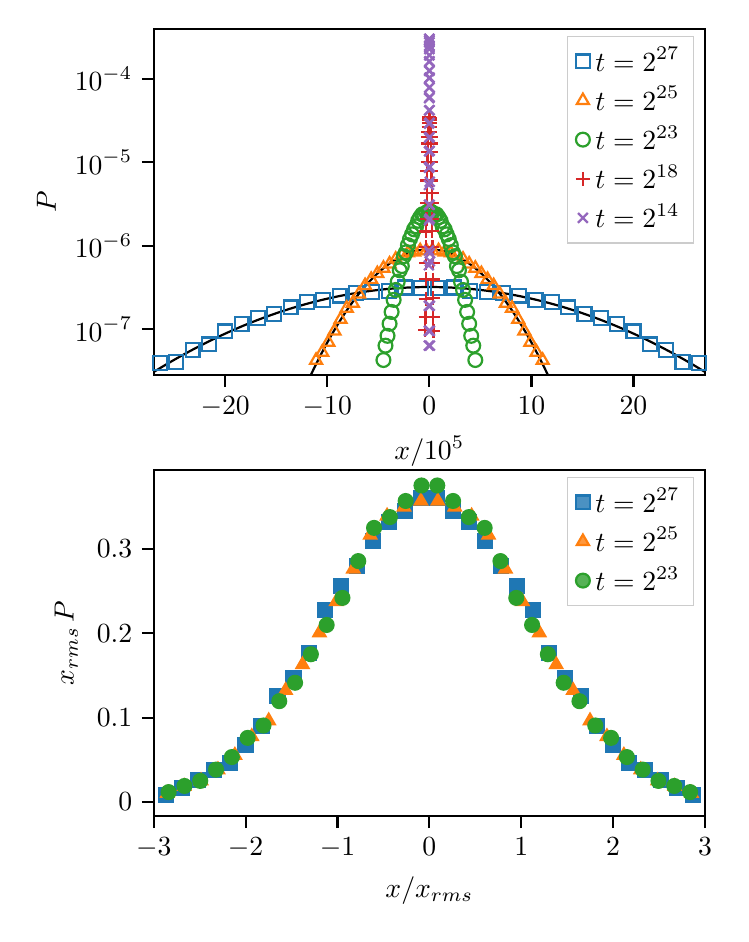
\begin{tikzpicture}

\definecolor{crimson2143940}{RGB}{214,39,40}
\definecolor{darkgrey176}{RGB}{176,176,176}
\definecolor{darkorange25512714}{RGB}{255,127,14}
\definecolor{forestgreen4416044}{RGB}{44,160,44}
\definecolor{lightgrey204}{RGB}{204,204,204}
\definecolor{mediumpurple148103189}{RGB}{148,103,189}
\definecolor{orchid227119194}{RGB}{227,119,194}
\definecolor{sienna1408675}{RGB}{140,86,75}
\definecolor{steelblue31119180}{RGB}{31,119,180}

\begin{groupplot}[group style={group size=1 by 2, vertical sep=1.2cm}, height=4.4cm, width=7cm]
\nextgroupplot[
legend cell align={left},
legend style={fill opacity=0.8, draw opacity=1, text opacity=1, draw=lightgrey204},
log basis y={10},
tick align=outside,
tick pos=left,
x grid style={darkgrey176},
xlabel={\(\displaystyle x/10^5\)},
xmin=-27, xmax=27,
xtick style={color=black},
y grid style={darkgrey176},
ylabel={\(\displaystyle  P \)},
ymin=2.8e-08, ymax=0.0004,
ymode=log,
ytick style={color=black},
ytick={1e-09,1e-08,1e-07,1e-06,1e-05,0.0001,0.001,0.01},
yticklabels={
  \(\displaystyle {10^{-9}}\),
  \(\displaystyle {10^{-8}}\),
  \(\displaystyle {10^{-7}}\),
  \(\displaystyle {10^{-6}}\),
  \(\displaystyle {10^{-5}}\),
  \(\displaystyle {10^{-4}}\),
  \(\displaystyle {10^{-3}}\),
  \(\displaystyle {10^{-2}}\)
}
]
\addplot [semithick, black, forget plot]
table {%
-30 1.77140129867429e-08
-29.9399399399399 1.79202612585694e-08
-29.8798798798799 1.81284903702559e-08
-29.8198198198198 1.83387136215314e-08
-29.7597597597598 1.85509443269235e-08
-29.6996996996997 1.87651958146873e-08
-29.6396396396396 1.89814814257204e-08
-29.5795795795796 1.91998145124637e-08
-29.5195195195195 1.94202084377885e-08
-29.4594594594595 1.96426765738695e-08
-29.3993993993994 1.98672323010433e-08
-29.3393393393393 2.00938890066533e-08
-29.2792792792793 2.03226600838809e-08
-29.2192192192192 2.05535589305617e-08
-29.1591591591592 2.07865989479887e-08
-29.0990990990991 2.10217935397004e-08
-29.039039039039 2.12591561102561e-08
-28.978978978979 2.14987000639963e-08
-28.9189189189189 2.17404388037894e-08
-28.8588588588589 2.19843857297646e-08
-28.7987987987988 2.22305542380304e-08
-28.7387387387387 2.24789577193799e-08
-28.6786786786787 2.27296095579813e-08
-28.6186186186186 2.29825231300554e-08
-28.5585585585586 2.32377118025387e-08
-28.4984984984985 2.34951889317331e-08
-28.4384384384384 2.3754967861941e-08
-28.3783783783784 2.4017061924088e-08
-28.3183183183183 2.42814844343306e-08
-28.2582582582583 2.45482486926512e-08
-28.1981981981982 2.48173679814389e-08
-28.1381381381381 2.5088855564057e-08
-28.0780780780781 2.5362724683397e-08
-28.018018018018 2.56389885604192e-08
-27.957957957958 2.59176603926794e-08
-27.8978978978979 2.61987533528434e-08
-27.8378378378378 2.6482280587187e-08
-27.7777777777778 2.67682552140833e-08
-27.7177177177177 2.70566903224772e-08
-27.6576576576577 2.73475989703463e-08
-27.5975975975976 2.76409941831491e-08
-27.5375375375375 2.79368889522602e-08
-27.4774774774775 2.82352962333928e-08
-27.4174174174174 2.85362289450081e-08
-27.3573573573574 2.88396999667126e-08
-27.2972972972973 2.91457221376421e-08
-27.2372372372372 2.94543082548341e-08
-27.1771771771772 2.9765471071587e-08
-27.1171171171171 3.00792232958076e-08
-27.0570570570571 3.03955775883457e-08
-26.996996996997 3.07145465613178e-08
-26.9369369369369 3.10361427764176e-08
-26.8768768768769 3.13603787432151e-08
-26.8168168168168 3.16872669174445e-08
-26.7567567567568 3.20168196992793e-08
-26.6966966966967 3.23490494315971e-08
-26.6366366366366 3.26839683982321e-08
-26.5765765765766 3.30215888222169e-08
-26.5165165165165 3.33619228640128e-08
-26.4564564564565 3.37049826197294e-08
-26.3963963963964 3.40507801193331e-08
-26.3363363363363 3.43993273248447e-08
-26.2762762762763 3.47506361285272e-08
-26.2162162162162 3.51047183510622e-08
-26.1561561561562 3.54615857397164e-08
-26.0960960960961 3.58212499664982e-08
-26.036036036036 3.6183722626304e-08
-25.975975975976 3.65490152350548e-08
-25.9159159159159 3.69171392278228e-08
-25.8558558558559 3.72881059569491e-08
-25.7957957957958 3.76619266901516e-08
-25.7357357357357 3.8038612608624e-08
-25.6756756756757 3.84181748051254e-08
-25.6156156156156 3.88006242820615e-08
-25.5555555555556 3.9185971949557e-08
-25.4954954954955 3.95742286235198e-08
-25.4354354354354 3.99654050236962e-08
-25.3753753753754 4.03595117717189e-08
-25.3153153153153 4.07565593891465e-08
-25.2552552552553 4.11565582954958e-08
-25.1951951951952 4.15595188062661e-08
-25.1351351351351 4.19654511309565e-08
-25.0750750750751 4.23743653710762e-08
-25.015015015015 4.27862715181479e-08
-24.954954954955 4.32011794517039e-08
-24.8948948948949 4.36190989372773e-08
-24.8348348348348 4.40400396243847e-08
-24.7747747747748 4.44640110445053e-08
-24.7147147147147 4.48910226090527e-08
-24.6546546546547 4.53210836073412e-08
-24.5945945945946 4.57542032045476e-08
-24.5345345345345 4.61903904396674e-08
-24.4744744744745 4.66296542234658e-08
-24.4144144144144 4.70720033364248e-08
-24.3543543543544 4.75174464266855e-08
-24.2942942942943 4.79659920079868e-08
-24.2342342342342 4.84176484575989e-08
-24.1741741741742 4.88724240142549e-08
-24.1141141141141 4.93303267760782e-08
-24.0540540540541 4.97913646985062e-08
-23.993993993994 5.02555455922125e-08
-23.9339339339339 5.07228771210255e-08
-23.8738738738739 5.11933667998449e-08
-23.8138138138138 5.16670219925564e-08
-23.7537537537538 5.21438499099446e-08
-23.6936936936937 5.26238576076038e-08
-23.6336336336336 5.31070519838487e-08
-23.5735735735736 5.35934397776232e-08
-23.5135135135135 5.40830275664087e-08
-23.4534534534535 5.45758217641324e-08
-23.3933933933934 5.50718286190758e-08
-23.3333333333333 5.55710542117819e-08
-23.2732732732733 5.60735044529649e-08
-23.2132132132132 5.65791850814194e-08
-23.1531531531532 5.70881016619311e-08
-23.0930930930931 5.76002595831887e-08
-23.033033033033 5.81156640556982e-08
-22.972972972973 5.8634320109698e-08
-22.9129129129129 5.91562325930775e-08
-22.8528528528529 5.96814061692981e-08
-22.7927927927928 6.02098453153163e-08
-22.7327327327327 6.07415543195111e-08
-22.6726726726727 6.12765372796147e-08
-22.6126126126126 6.18147981006467e-08
-22.5525525525526 6.2356340492853e-08
-22.4924924924925 6.29011679696492e-08
-22.4324324324324 6.34492838455686e-08
-22.3723723723724 6.40006912342159e-08
-22.3123123123123 6.45553930462256e-08
-22.2522522522523 6.51133919872276e-08
-22.1921921921922 6.56746905558177e-08
-22.1321321321321 6.62392910415354e-08
-22.0720720720721 6.68071955228485e-08
-22.012012012012 6.73784058651447e-08
-21.951951951952 6.7952923718731e-08
-21.8918918918919 6.85307505168411e-08
-21.8318318318318 6.91118874736507e-08
-21.7717717717718 6.96963355823015e-08
-21.7117117117117 7.0284095612935e-08
-21.6516516516517 7.08751681107343e-08
-21.5915915915916 7.14695533939762e-08
-21.5315315315315 7.20672515520938e-08
-21.4714714714715 7.26682624437486e-08
-21.4114114114114 7.32725856949138e-08
-21.3513513513514 7.3880220696969e-08
-21.2912912912913 7.44911666048054e-08
-21.2312312312312 7.5105422334944e-08
-21.1711711711712 7.57229865636651e-08
-21.1111111111111 7.63438577251504e-08
-21.0510510510511 7.69680340096387e-08
-20.990990990991 7.7595513361594e-08
-20.9309309309309 7.82262934778878e-08
-20.8708708708709 7.88603718059953e-08
-20.8108108108108 7.94977455422057e-08
-20.7507507507508 8.01384116298471e-08
-20.6906906906907 8.07823667575276e-08
-20.6306306306306 8.14296073573902e-08
-20.5705705705706 8.2080129603385e-08
-20.5105105105105 8.27339294095565e-08
-20.4504504504505 8.33910024283484e-08
-20.3903903903904 8.40513440489244e-08
-20.3303303303303 8.47149493955073e-08
-20.2702702702703 8.53818133257348e-08
-20.2102102102102 8.60519304290343e-08
-20.1501501501502 8.67252950250151e-08
-20.0900900900901 8.74019011618802e-08
-20.03003003003 8.80817426148572e-08
-19.96996996997 8.8764812884648e-08
-19.9099099099099 8.94511051958992e-08
-19.8498498498498 9.01406124956924e-08
-19.7897897897898 9.08333274520553e-08
-19.7297297297297 9.15292424524933e-08
-19.6696696696697 9.22283496025432e-08
-19.6096096096096 9.29306407243482e-08
-19.5495495495495 9.36361073552548e-08
-19.4894894894895 9.43447407464331e-08
-19.4294294294294 9.50565318615183e-08
-19.3693693693694 9.5771471375277e-08
-19.3093093093093 9.64895496722965e-08
-19.2492492492492 9.72107568456973e-08
-19.1891891891892 9.79350826958708e-08
-19.1291291291291 9.86625167292415e-08
-19.0690690690691 9.93930481570537e-08
-19.009009009009 1.00126665894184e-07
-18.9489489489489 1.00863358557978e-07
-18.8888888888889 1.01603114467118e-07
-18.8288288288288 1.0234592164051e-07
-18.7687687687688 1.030917677962e-07
-18.7087087087087 1.03840640350323e-07
-18.6486486486486 1.04592526416071e-07
-18.5885885885886 1.05347412802693e-07
-18.5285285285285 1.06105286014524e-07
-18.4684684684685 1.0686613225004e-07
-18.4084084084084 1.07629937400943e-07
-18.3483483483483 1.08396687051275e-07
-18.2882882882883 1.09166366476564e-07
-18.2282282282282 1.09938960642993e-07
-18.1681681681682 1.10714454206605e-07
-18.1081081081081 1.1149283151254e-07
-18.048048048048 1.12274076594297e-07
-17.987987987988 1.13058173173027e-07
-17.9279279279279 1.13845104656867e-07
-17.8678678678679 1.14634854140293e-07
-17.8078078078078 1.15427404403513e-07
-17.7477477477477 1.16222737911892e-07
-17.6876876876877 1.17020836815406e-07
-17.6276276276276 1.1782168294813e-07
-17.5675675675676 1.18625257827764e-07
-17.5075075075075 1.19431542655182e-07
-17.4474474474474 1.20240518314031e-07
-17.3873873873874 1.21052165370346e-07
-17.3273273273273 1.21866464072212e-07
-17.2672672672673 1.22683394349458e-07
-17.2072072072072 1.23502935813381e-07
-17.1471471471471 1.24325067756512e-07
-17.0870870870871 1.25149769152414e-07
-17.027027027027 1.25977018655515e-07
-16.966966966967 1.2680679460098e-07
-16.9069069069069 1.27639075004617e-07
-16.8468468468468 1.28473837562817e-07
-16.7867867867868 1.29311059652542e-07
-16.7267267267267 1.30150718331332e-07
-16.6666666666667 1.30992790337368e-07
-16.6066066066066 1.31837252089558e-07
-16.5465465465465 1.32684079687667e-07
-16.4864864864865 1.3353324891249e-07
-16.4264264264264 1.3438473522605e-07
-16.3663663663664 1.35238513771849e-07
-16.3063063063063 1.36094559375145e-07
-16.2462462462462 1.36952846543277e-07
-16.1861861861862 1.37813349466025e-07
-16.1261261261261 1.38676042016011e-07
-16.0660660660661 1.39540897749133e-07
-16.006006006006 1.40407889905052e-07
-15.9459459459459 1.41276991407704e-07
-15.8858858858859 1.4214817486586e-07
-15.8258258258258 1.43021412573729e-07
-15.7657657657658 1.43896676511592e-07
-15.7057057057057 1.44773938346481e-07
-15.6456456456456 1.45653169432905e-07
-15.5855855855856 1.46534340813605e-07
-15.5255255255255 1.47417423220358e-07
-15.4654654654655 1.48302387074822e-07
-15.4054054054054 1.49189202489415e-07
-15.3453453453453 1.50077839268243e-07
-15.2852852852853 1.50968266908069e-07
-15.2252252252252 1.51860454599318e-07
-15.1651651651652 1.52754371227125e-07
-15.1051051051051 1.53649985372434e-07
-15.045045045045 1.54547265313123e-07
-14.984984984985 1.55446179025183e-07
-14.9249249249249 1.56346694183938e-07
-14.8648648648649 1.57248778165299e-07
-14.8048048048048 1.5815239804707e-07
-14.7447447447447 1.59057520610287e-07
-14.6846846846847 1.5996411234061e-07
-14.6246246246246 1.60872139429745e-07
-14.5645645645646 1.61781567776922e-07
-14.5045045045045 1.62692362990398e-07
-14.4444444444444 1.63604490389023e-07
-14.3843843843844 1.6451791500383e-07
-14.3243243243243 1.65432601579679e-07
-14.2642642642643 1.6634851457694e-07
-14.2042042042042 1.67265618173216e-07
-14.1441441441441 1.68183876265113e-07
-14.0840840840841 1.69103252470048e-07
-14.024024024024 1.70023710128104e-07
-13.963963963964 1.70945212303922e-07
-13.9039039039039 1.71867721788642e-07
-13.8438438438438 1.7279120110188e-07
-13.7837837837838 1.7371561249375e-07
-13.7237237237237 1.74640917946929e-07
-13.6636636636637 1.75567079178765e-07
-13.6036036036036 1.76494057643422e-07
-13.5435435435435 1.77421814534072e-07
-13.4834834834835 1.78350310785129e-07
-13.4234234234234 1.79279507074523e-07
-13.3633633633634 1.80209363826011e-07
-13.3033033033033 1.81139841211544e-07
-13.2432432432432 1.82070899153657e-07
-13.1831831831832 1.83002497327916e-07
-13.1231231231231 1.83934595165396e-07
-13.0630630630631 1.84867151855207e-07
-13.003003003003 1.85800126347057e-07
-12.9429429429429 1.86733477353856e-07
-12.8828828828829 1.87667163354364e-07
-12.8228228228228 1.88601142595873e-07
-12.7627627627628 1.8953537309694e-07
-12.7027027027027 1.9046981265015e-07
-12.6426426426426 1.9140441882492e-07
-12.5825825825826 1.92339148970352e-07
-12.5225225225225 1.93273960218116e-07
-12.4624624624625 1.94208809485374e-07
-12.4024024024024 1.95143653477749e-07
-12.3423423423423 1.96078448692326e-07
-12.2822822822823 1.97013151420694e-07
-12.2222222222222 1.9794771775203e-07
-12.1621621621622 1.98882103576216e-07
-12.1021021021021 1.99816264586997e-07
-12.042042042042 2.00750156285178e-07
-11.981981981982 2.01683733981852e-07
-11.9219219219219 2.02616952801675e-07
-11.8618618618619 2.03549767686169e-07
-11.8018018018018 2.04482133397067e-07
-11.7417417417417 2.05414004519693e-07
-11.6816816816817 2.06345335466377e-07
-11.6216216216216 2.07276080479905e-07
-11.5615615615616 2.08206193637009e-07
-11.5015015015015 2.09135628851887e-07
-11.4414414414414 2.1006433987976e-07
-11.3813813813814 2.10992280320462e-07
-11.3213213213213 2.11919403622067e-07
-11.2612612612613 2.12845663084545e-07
-11.2012012012012 2.13771011863458e-07
-11.1411411411411 2.14695402973682e-07
-11.0810810810811 2.15618789293166e-07
-11.021021021021 2.1654112356672e-07
-10.960960960961 2.17462358409841e-07
-10.9009009009009 2.18382446312562e-07
-10.8408408408408 2.19301339643335e-07
-10.7807807807808 2.20218990652953e-07
-10.7207207207207 2.21135351478487e-07
-10.6606606606607 2.22050374147264e-07
-10.6006006006006 2.22964010580872e-07
-10.5405405405405 2.23876212599193e-07
-10.4804804804805 2.2478693192446e-07
-10.4204204204204 2.25696120185353e-07
-10.3603603603604 2.26603728921111e-07
-10.3003003003003 2.2750970958568e-07
-10.2402402402402 2.28414013551879e-07
-10.1801801801802 2.29316592115602e-07
-10.1201201201201 2.30217396500036e-07
-10.0600600600601 2.31116377859912e-07
-10 2.32013487285776e-07
-9.93993993993994 2.32908675808286e-07
-9.87987987987988 2.33801894402532e-07
-9.81981981981982 2.34693093992379e-07
-9.75975975975976 2.35582225454835e-07
-9.6996996996997 2.36469239624437e-07
-9.63963963963964 2.37354087297662e-07
-9.57957957957958 2.38236719237359e-07
-9.51951951951952 2.39117086177197e-07
-9.45945945945946 2.39995138826141e-07
-9.3993993993994 2.40870827872941e-07
-9.33933933933934 2.41744103990641e-07
-9.27927927927928 2.42614917841106e-07
-9.21921921921922 2.43483220079573e-07
-9.15915915915916 2.44348961359209e-07
-9.0990990990991 2.45212092335694e-07
-9.03903903903904 2.46072563671813e-07
-8.97897897897898 2.46930326042072e-07
-8.91891891891892 2.47785330137322e-07
-8.85885885885886 2.48637526669398e-07
-8.7987987987988 2.49486866375776e-07
-8.73873873873874 2.50333300024237e-07
-8.67867867867868 2.51176778417548e-07
-8.61861861861862 2.52017252398157e-07
-8.55855855855856 2.5285467285289e-07
-8.4984984984985 2.53688990717667e-07
-8.43843843843844 2.54520156982225e-07
-8.37837837837838 2.55348122694855e-07
-8.31831831831832 2.56172838967134e-07
-8.25825825825826 2.56994256978686e-07
-8.1981981981982 2.57812327981931e-07
-8.13813813813814 2.58627003306852e-07
-8.07807807807808 2.59438234365766e-07
-8.01801801801802 2.60245972658097e-07
-7.95795795795796 2.6105016977516e-07
-7.8978978978979 2.61850777404946e-07
-7.83783783783784 2.62647747336906e-07
-7.77777777777778 2.63441031466749e-07
-7.71771771771772 2.6423058180123e-07
-7.65765765765766 2.65016350462949e-07
-7.5975975975976 2.65798289695149e-07
-7.53753753753754 2.66576351866506e-07
-7.47747747747748 2.67350489475934e-07
-7.41741741741742 2.68120655157374e-07
-7.35735735735736 2.6888680168459e-07
-7.2972972972973 2.6964888197596e-07
-7.23723723723724 2.70406849099265e-07
-7.17717717717718 2.71160656276474e-07
-7.11711711711712 2.71910256888521e-07
-7.05705705705706 2.72655604480083e-07
-6.996996996997 2.73396652764348e-07
-6.93693693693694 2.74133355627779e-07
-6.87687687687688 2.74865667134869e-07
-6.81681681681682 2.75593541532888e-07
-6.75675675675676 2.76316933256624e-07
-6.6966966966967 2.7703579693311e-07
-6.63663663663664 2.77750087386351e-07
-6.57657657657658 2.78459759642026e-07
-6.51651651651652 2.79164768932193e-07
-6.45645645645646 2.7986507069997e-07
-6.3963963963964 2.80560620604215e-07
-6.33633633633634 2.81251374524181e-07
-6.27627627627628 2.81937288564169e-07
-6.21621621621622 2.82618319058155e-07
-6.15615615615616 2.83294422574409e-07
-6.0960960960961 2.83965555920096e-07
-6.03603603603604 2.8463167614586e-07
-5.97597597597598 2.85292740550392e-07
-5.91591591591592 2.85948706684976e-07
-5.85585585585586 2.86599532358022e-07
-5.7957957957958 2.87245175639576e-07
-5.73573573573574 2.87885594865809e-07
-5.67567567567568 2.88520748643489e-07
-5.61561561561562 2.89150595854428e-07
-5.55555555555556 2.8977509565991e-07
-5.4954954954955 2.90394207505094e-07
-5.43543543543544 2.91007891123393e-07
-5.37537537537538 2.91616106540833e-07
-5.31531531531532 2.92218814080382e-07
-5.25525525525526 2.92815974366258e-07
-5.1951951951952 2.93407548328206e-07
-5.13513513513514 2.93993497205756e-07
-5.07507507507508 2.94573782552447e-07
-5.01501501501502 2.95148366240024e-07
-4.95495495495496 2.95717210462608e-07
-4.8948948948949 2.96280277740838e-07
-4.83483483483484 2.96837530925981e-07
-4.77477477477478 2.97388933204009e-07
-4.71471471471472 2.97934448099652e-07
-4.65465465465466 2.98474039480411e-07
-4.5945945945946 2.99007671560547e-07
-4.53453453453454 2.99535308905029e-07
-4.47447447447448 3.00056916433452e-07
-4.41441441441442 3.00572459423925e-07
-4.35435435435435 3.01081903516915e-07
-4.29429429429429 3.01585214719062e-07
-4.23423423423423 3.02082359406961e-07
-4.17417417417417 3.02573304330894e-07
-4.11411411411411 3.03058016618544e-07
-4.05405405405405 3.03536463778654e-07
-3.99399399399399 3.04008613704657e-07
-3.93393393393393 3.04474434678266e-07
-3.87387387387387 3.04933895373021e-07
-3.81381381381381 3.05386964857801e-07
-3.75375375375375 3.0583361260029e-07
-3.69369369369369 3.0627380847041e-07
-3.63363363363363 3.06707522743699e-07
-3.57357357357357 3.07134726104664e-07
-3.51351351351351 3.07555389650075e-07
-3.45345345345345 3.07969484892228e-07
-3.39339339339339 3.08376983762155e-07
-3.33333333333333 3.08777858612798e-07
-3.27327327327327 3.09172082222133e-07
-3.21321321321321 3.0955962779625e-07
-3.15315315315315 3.09940468972387e-07
-3.09309309309309 3.10314579821918e-07
-3.03303303303303 3.10681934853297e-07
-2.97297297297297 3.11042509014947e-07
-2.91291291291291 3.11396277698115e-07
-2.85285285285285 3.11743216739663e-07
-2.79279279279279 3.12083302424821e-07
-2.73273273273273 3.12416511489892e-07
-2.67267267267267 3.12742821124896e-07
-2.61261261261261 3.1306220897618e-07
-2.55255255255255 3.13374653148965e-07
-2.49249249249249 3.1368013220985e-07
-2.43243243243243 3.13978625189261e-07
-2.37237237237237 3.1427011158385e-07
-2.31231231231231 3.14554571358841e-07
-2.25225225225225 3.14831984950328e-07
-2.19219219219219 3.15102333267514e-07
-2.13213213213213 3.15365597694904e-07
-2.07207207207207 3.15621760094436e-07
-2.01201201201201 3.15870802807572e-07
-1.95195195195195 3.16112708657316e-07
-1.89189189189189 3.16347460950197e-07
-1.83183183183183 3.16575043478187e-07
-1.77177177177177 3.16795440520564e-07
-1.71171171171171 3.17008636845721e-07
-1.65165165165165 3.17214617712925e-07
-1.59159159159159 3.17413368874012e-07
-1.53153153153153 3.17604876575031e-07
-1.47147147147147 3.17789127557828e-07
-1.41141141141141 3.17966109061579e-07
-1.35135135135135 3.18135808824261e-07
-1.29129129129129 3.1829821508407e-07
-1.23123123123123 3.18453316580776e-07
-1.17117117117117 3.18601102557026e-07
-1.11111111111111 3.18741562759591e-07
-1.05105105105105 3.18874687440543e-07
-0.990990990990991 3.19000467358393e-07
-0.930930930930931 3.19118893779152e-07
-0.870870870870871 3.19229958477346e-07
-0.810810810810811 3.19333653736967e-07
-0.75075075075075 3.19429972352365e-07
-0.69069069069069 3.19518907629085e-07
-0.63063063063063 3.19600453384642e-07
-0.57057057057057 3.19674603949235e-07
-0.51051051051051 3.19741354166408e-07
-0.45045045045045 3.19800699393644e-07
-0.39039039039039 3.19852635502903e-07
-0.33033033033033 3.19897158881106e-07
-0.27027027027027 3.19934266430545e-07
-0.21021021021021 3.19963955569252e-07
-0.15015015015015 3.19986224231291e-07
-0.0900900900900901 3.20001070866999e-07
-0.03003003003003 3.2000849444317e-07
0.03003003003003 3.2000849444317e-07
0.0900900900900901 3.20001070866999e-07
0.15015015015015 3.19986224231291e-07
0.21021021021021 3.19963955569252e-07
0.27027027027027 3.19934266430545e-07
0.33033033033033 3.19897158881106e-07
0.39039039039039 3.19852635502903e-07
0.45045045045045 3.19800699393644e-07
0.51051051051051 3.19741354166408e-07
0.57057057057057 3.19674603949235e-07
0.63063063063063 3.19600453384642e-07
0.69069069069069 3.19518907629085e-07
0.75075075075075 3.19429972352365e-07
0.810810810810811 3.19333653736967e-07
0.870870870870871 3.19229958477346e-07
0.930930930930931 3.19118893779152e-07
0.990990990990991 3.19000467358393e-07
1.05105105105105 3.18874687440543e-07
1.11111111111111 3.18741562759591e-07
1.17117117117117 3.18601102557026e-07
1.23123123123123 3.18453316580776e-07
1.29129129129129 3.1829821508407e-07
1.35135135135135 3.18135808824261e-07
1.41141141141141 3.17966109061579e-07
1.47147147147147 3.17789127557828e-07
1.53153153153153 3.17604876575031e-07
1.59159159159159 3.17413368874012e-07
1.65165165165165 3.17214617712925e-07
1.71171171171171 3.17008636845721e-07
1.77177177177177 3.16795440520564e-07
1.83183183183183 3.16575043478187e-07
1.89189189189189 3.16347460950197e-07
1.95195195195195 3.16112708657316e-07
2.01201201201201 3.15870802807572e-07
2.07207207207207 3.15621760094436e-07
2.13213213213213 3.15365597694904e-07
2.19219219219219 3.15102333267514e-07
2.25225225225226 3.14831984950328e-07
2.31231231231232 3.14554571358841e-07
2.37237237237238 3.1427011158385e-07
2.43243243243244 3.13978625189261e-07
2.4924924924925 3.1368013220985e-07
2.55255255255256 3.13374653148965e-07
2.61261261261262 3.1306220897618e-07
2.67267267267268 3.12742821124896e-07
2.73273273273274 3.12416511489892e-07
2.7927927927928 3.12083302424821e-07
2.85285285285286 3.11743216739663e-07
2.91291291291292 3.11396277698115e-07
2.97297297297298 3.11042509014947e-07
3.03303303303304 3.10681934853296e-07
3.0930930930931 3.10314579821918e-07
3.15315315315316 3.09940468972387e-07
3.21321321321322 3.0955962779625e-07
3.27327327327328 3.09172082222133e-07
3.33333333333334 3.08777858612798e-07
3.3933933933934 3.08376983762155e-07
3.45345345345346 3.07969484892228e-07
3.51351351351352 3.07555389650075e-07
3.57357357357358 3.07134726104664e-07
3.63363363363364 3.06707522743699e-07
3.6936936936937 3.0627380847041e-07
3.75375375375376 3.0583361260029e-07
3.81381381381382 3.053869648578e-07
3.87387387387388 3.04933895373021e-07
3.93393393393394 3.04474434678266e-07
3.993993993994 3.04008613704657e-07
4.05405405405406 3.03536463778654e-07
4.11411411411412 3.03058016618544e-07
4.17417417417418 3.02573304330894e-07
4.23423423423424 3.0208235940696e-07
4.2942942942943 3.01585214719062e-07
4.35435435435436 3.01081903516915e-07
4.41441441441442 3.00572459423925e-07
4.47447447447448 3.00056916433452e-07
4.53453453453454 2.99535308905029e-07
4.5945945945946 2.99007671560547e-07
4.65465465465466 2.98474039480411e-07
4.71471471471472 2.97934448099652e-07
4.77477477477478 2.97388933204009e-07
4.83483483483484 2.96837530925981e-07
4.8948948948949 2.96280277740838e-07
4.95495495495496 2.95717210462608e-07
5.01501501501502 2.95148366240024e-07
5.07507507507508 2.94573782552447e-07
5.13513513513514 2.93993497205756e-07
5.1951951951952 2.93407548328206e-07
5.25525525525526 2.92815974366258e-07
5.31531531531532 2.92218814080382e-07
5.37537537537538 2.91616106540833e-07
5.43543543543544 2.91007891123393e-07
5.4954954954955 2.90394207505094e-07
5.55555555555556 2.8977509565991e-07
5.61561561561562 2.89150595854428e-07
5.67567567567568 2.88520748643489e-07
5.73573573573574 2.87885594865809e-07
5.7957957957958 2.87245175639576e-07
5.85585585585586 2.86599532358022e-07
5.91591591591592 2.85948706684976e-07
5.97597597597598 2.85292740550392e-07
6.03603603603604 2.8463167614586e-07
6.0960960960961 2.83965555920096e-07
6.15615615615616 2.83294422574409e-07
6.21621621621622 2.82618319058155e-07
6.27627627627628 2.81937288564169e-07
6.33633633633634 2.81251374524181e-07
6.3963963963964 2.80560620604215e-07
6.45645645645646 2.7986507069997e-07
6.51651651651652 2.79164768932193e-07
6.57657657657658 2.78459759642026e-07
6.63663663663664 2.77750087386351e-07
6.6966966966967 2.7703579693311e-07
6.75675675675676 2.76316933256624e-07
6.81681681681682 2.75593541532888e-07
6.87687687687688 2.74865667134869e-07
6.93693693693694 2.74133355627779e-07
6.996996996997 2.73396652764348e-07
7.05705705705706 2.72655604480083e-07
7.11711711711712 2.71910256888521e-07
7.17717717717718 2.71160656276474e-07
7.23723723723724 2.70406849099265e-07
7.2972972972973 2.6964888197596e-07
7.35735735735736 2.6888680168459e-07
7.41741741741742 2.68120655157374e-07
7.47747747747748 2.67350489475934e-07
7.53753753753754 2.66576351866506e-07
7.5975975975976 2.65798289695149e-07
7.65765765765766 2.65016350462949e-07
7.71771771771772 2.6423058180123e-07
7.77777777777778 2.63441031466749e-07
7.83783783783784 2.62647747336906e-07
7.8978978978979 2.61850777404946e-07
7.95795795795796 2.6105016977516e-07
8.01801801801802 2.60245972658097e-07
8.07807807807808 2.59438234365766e-07
8.13813813813814 2.58627003306852e-07
8.1981981981982 2.57812327981931e-07
8.25825825825826 2.56994256978686e-07
8.31831831831832 2.56172838967134e-07
8.37837837837838 2.55348122694855e-07
8.43843843843844 2.54520156982225e-07
8.4984984984985 2.53688990717667e-07
8.55855855855856 2.5285467285289e-07
8.61861861861862 2.52017252398157e-07
8.67867867867868 2.51176778417548e-07
8.73873873873874 2.50333300024237e-07
8.7987987987988 2.49486866375776e-07
8.85885885885886 2.48637526669398e-07
8.91891891891892 2.47785330137322e-07
8.97897897897898 2.46930326042072e-07
9.03903903903904 2.46072563671813e-07
9.0990990990991 2.45212092335694e-07
9.15915915915916 2.44348961359209e-07
9.21921921921922 2.43483220079573e-07
9.27927927927928 2.42614917841106e-07
9.33933933933934 2.41744103990641e-07
9.3993993993994 2.40870827872941e-07
9.45945945945946 2.39995138826141e-07
9.51951951951952 2.39117086177197e-07
9.57957957957958 2.38236719237359e-07
9.63963963963964 2.37354087297662e-07
9.6996996996997 2.36469239624437e-07
9.75975975975976 2.35582225454835e-07
9.81981981981982 2.34693093992379e-07
9.87987987987988 2.33801894402532e-07
9.93993993993994 2.32908675808286e-07
10 2.32013487285776e-07
10.0600600600601 2.31116377859912e-07
10.1201201201201 2.30217396500036e-07
10.1801801801802 2.29316592115602e-07
10.2402402402402 2.28414013551879e-07
10.3003003003003 2.2750970958568e-07
10.3603603603604 2.26603728921111e-07
10.4204204204204 2.25696120185353e-07
10.4804804804805 2.2478693192446e-07
10.5405405405405 2.23876212599193e-07
10.6006006006006 2.22964010580872e-07
10.6606606606607 2.22050374147264e-07
10.7207207207207 2.21135351478487e-07
10.7807807807808 2.20218990652953e-07
10.8408408408408 2.19301339643335e-07
10.9009009009009 2.18382446312562e-07
10.960960960961 2.17462358409841e-07
11.021021021021 2.1654112356672e-07
11.0810810810811 2.15618789293166e-07
11.1411411411411 2.14695402973682e-07
11.2012012012012 2.13771011863458e-07
11.2612612612613 2.12845663084545e-07
11.3213213213213 2.11919403622067e-07
11.3813813813814 2.10992280320462e-07
11.4414414414414 2.1006433987976e-07
11.5015015015015 2.09135628851887e-07
11.5615615615616 2.08206193637009e-07
11.6216216216216 2.07276080479905e-07
11.6816816816817 2.06345335466377e-07
11.7417417417417 2.05414004519693e-07
11.8018018018018 2.04482133397067e-07
11.8618618618619 2.03549767686169e-07
11.9219219219219 2.02616952801675e-07
11.981981981982 2.01683733981852e-07
12.042042042042 2.00750156285178e-07
12.1021021021021 1.99816264586997e-07
12.1621621621622 1.98882103576216e-07
12.2222222222222 1.9794771775203e-07
12.2822822822823 1.97013151420694e-07
12.3423423423423 1.96078448692326e-07
12.4024024024024 1.95143653477749e-07
12.4624624624625 1.94208809485374e-07
12.5225225225225 1.93273960218116e-07
12.5825825825826 1.92339148970352e-07
12.6426426426426 1.9140441882492e-07
12.7027027027027 1.9046981265015e-07
12.7627627627628 1.8953537309694e-07
12.8228228228228 1.88601142595873e-07
12.8828828828829 1.87667163354364e-07
12.9429429429429 1.86733477353856e-07
13.003003003003 1.85800126347057e-07
13.0630630630631 1.84867151855207e-07
13.1231231231231 1.83934595165396e-07
13.1831831831832 1.83002497327916e-07
13.2432432432432 1.82070899153657e-07
13.3033033033033 1.81139841211544e-07
13.3633633633634 1.80209363826011e-07
13.4234234234234 1.79279507074523e-07
13.4834834834835 1.78350310785129e-07
13.5435435435435 1.77421814534072e-07
13.6036036036036 1.76494057643422e-07
13.6636636636637 1.75567079178765e-07
13.7237237237237 1.74640917946929e-07
13.7837837837838 1.7371561249375e-07
13.8438438438438 1.7279120110188e-07
13.9039039039039 1.71867721788642e-07
13.963963963964 1.70945212303922e-07
14.024024024024 1.70023710128104e-07
14.0840840840841 1.69103252470048e-07
14.1441441441441 1.68183876265113e-07
14.2042042042042 1.67265618173216e-07
14.2642642642643 1.6634851457694e-07
14.3243243243243 1.65432601579679e-07
14.3843843843844 1.6451791500383e-07
14.4444444444444 1.63604490389023e-07
14.5045045045045 1.62692362990398e-07
14.5645645645646 1.61781567776922e-07
14.6246246246246 1.60872139429745e-07
14.6846846846847 1.5996411234061e-07
14.7447447447447 1.59057520610287e-07
14.8048048048048 1.5815239804707e-07
14.8648648648649 1.57248778165299e-07
14.9249249249249 1.56346694183938e-07
14.984984984985 1.55446179025183e-07
15.045045045045 1.54547265313123e-07
15.1051051051051 1.53649985372434e-07
15.1651651651652 1.52754371227125e-07
15.2252252252252 1.51860454599318e-07
15.2852852852853 1.50968266908069e-07
15.3453453453453 1.50077839268243e-07
15.4054054054054 1.49189202489415e-07
15.4654654654655 1.48302387074822e-07
15.5255255255255 1.47417423220358e-07
15.5855855855856 1.46534340813605e-07
15.6456456456456 1.45653169432905e-07
15.7057057057057 1.44773938346481e-07
15.7657657657658 1.43896676511592e-07
15.8258258258258 1.43021412573729e-07
15.8858858858859 1.4214817486586e-07
15.9459459459459 1.41276991407704e-07
16.006006006006 1.40407889905052e-07
16.0660660660661 1.39540897749133e-07
16.1261261261261 1.38676042016011e-07
16.1861861861862 1.37813349466025e-07
16.2462462462462 1.36952846543277e-07
16.3063063063063 1.36094559375145e-07
16.3663663663664 1.35238513771849e-07
16.4264264264264 1.3438473522605e-07
16.4864864864865 1.3353324891249e-07
16.5465465465465 1.32684079687667e-07
16.6066066066066 1.31837252089558e-07
16.6666666666667 1.30992790337368e-07
16.7267267267267 1.30150718331332e-07
16.7867867867868 1.29311059652542e-07
16.8468468468468 1.28473837562817e-07
16.9069069069069 1.27639075004617e-07
16.966966966967 1.2680679460098e-07
17.027027027027 1.25977018655515e-07
17.0870870870871 1.25149769152414e-07
17.1471471471471 1.24325067756512e-07
17.2072072072072 1.23502935813381e-07
17.2672672672673 1.22683394349458e-07
17.3273273273273 1.21866464072212e-07
17.3873873873874 1.21052165370346e-07
17.4474474474474 1.20240518314031e-07
17.5075075075075 1.19431542655182e-07
17.5675675675676 1.18625257827764e-07
17.6276276276276 1.1782168294813e-07
17.6876876876877 1.17020836815406e-07
17.7477477477477 1.16222737911892e-07
17.8078078078078 1.15427404403513e-07
17.8678678678679 1.14634854140293e-07
17.9279279279279 1.13845104656867e-07
17.987987987988 1.13058173173027e-07
18.048048048048 1.12274076594297e-07
18.1081081081081 1.11492831512541e-07
18.1681681681682 1.10714454206605e-07
18.2282282282282 1.09938960642993e-07
18.2882882882883 1.09166366476564e-07
18.3483483483483 1.08396687051275e-07
18.4084084084084 1.07629937400943e-07
18.4684684684685 1.0686613225004e-07
18.5285285285285 1.06105286014524e-07
18.5885885885886 1.05347412802693e-07
18.6486486486486 1.04592526416071e-07
18.7087087087087 1.03840640350323e-07
18.7687687687688 1.030917677962e-07
18.8288288288288 1.0234592164051e-07
18.8888888888889 1.01603114467119e-07
18.9489489489489 1.00863358557978e-07
19.009009009009 1.00126665894184e-07
19.0690690690691 9.93930481570537e-08
19.1291291291291 9.86625167292416e-08
19.1891891891892 9.79350826958708e-08
19.2492492492492 9.72107568456973e-08
19.3093093093093 9.64895496722965e-08
19.3693693693694 9.57714713752771e-08
19.4294294294294 9.50565318615183e-08
19.4894894894895 9.43447407464331e-08
19.5495495495495 9.36361073552549e-08
19.6096096096096 9.29306407243482e-08
19.6696696696697 9.22283496025432e-08
19.7297297297297 9.15292424524933e-08
19.7897897897898 9.08333274520553e-08
19.8498498498498 9.01406124956925e-08
19.9099099099099 8.94511051958992e-08
19.96996996997 8.8764812884648e-08
20.03003003003 8.80817426148572e-08
20.0900900900901 8.74019011618802e-08
20.1501501501501 8.67252950250151e-08
20.2102102102102 8.60519304290343e-08
20.2702702702703 8.53818133257349e-08
20.3303303303303 8.47149493955073e-08
20.3903903903904 8.40513440489244e-08
20.4504504504504 8.33910024283484e-08
20.5105105105105 8.27339294095565e-08
20.5705705705706 8.2080129603385e-08
20.6306306306306 8.14296073573902e-08
20.6906906906907 8.07823667575276e-08
20.7507507507507 8.01384116298471e-08
20.8108108108108 7.94977455422057e-08
20.8708708708709 7.88603718059954e-08
20.9309309309309 7.82262934778879e-08
20.990990990991 7.7595513361594e-08
21.051051051051 7.69680340096387e-08
21.1111111111111 7.63438577251504e-08
21.1711711711712 7.57229865636652e-08
21.2312312312312 7.51054223349441e-08
21.2912912912913 7.44911666048054e-08
21.3513513513514 7.38802206969689e-08
21.4114114114114 7.32725856949138e-08
21.4714714714715 7.26682624437485e-08
21.5315315315315 7.20672515520937e-08
21.5915915915916 7.14695533939762e-08
21.6516516516517 7.08751681107343e-08
21.7117117117117 7.0284095612935e-08
21.7717717717718 6.96963355823015e-08
21.8318318318318 6.91118874736506e-08
21.8918918918919 6.8530750516841e-08
21.951951951952 6.7952923718731e-08
22.012012012012 6.73784058651446e-08
22.0720720720721 6.68071955228484e-08
22.1321321321321 6.62392910415353e-08
22.1921921921922 6.56746905558176e-08
22.2522522522523 6.51133919872275e-08
22.3123123123123 6.45553930462255e-08
22.3723723723724 6.40006912342158e-08
22.4324324324324 6.34492838455686e-08
22.4924924924925 6.29011679696491e-08
22.5525525525526 6.2356340492853e-08
22.6126126126126 6.18147981006466e-08
22.6726726726727 6.12765372796147e-08
22.7327327327327 6.07415543195111e-08
22.7927927927928 6.02098453153162e-08
22.8528528528529 5.96814061692981e-08
22.9129129129129 5.91562325930775e-08
22.972972972973 5.86343201096979e-08
23.033033033033 5.81156640556982e-08
23.0930930930931 5.76002595831887e-08
23.1531531531532 5.70881016619311e-08
23.2132132132132 5.65791850814194e-08
23.2732732732733 5.60735044529649e-08
23.3333333333333 5.55710542117818e-08
23.3933933933934 5.50718286190757e-08
23.4534534534535 5.45758217641324e-08
23.5135135135135 5.40830275664086e-08
23.5735735735736 5.35934397776232e-08
23.6336336336336 5.31070519838487e-08
23.6936936936937 5.26238576076038e-08
23.7537537537538 5.21438499099446e-08
23.8138138138138 5.16670219925564e-08
23.8738738738739 5.11933667998449e-08
23.9339339339339 5.07228771210255e-08
23.993993993994 5.02555455922125e-08
24.0540540540541 4.97913646985062e-08
24.1141141141141 4.93303267760782e-08
24.1741741741742 4.88724240142549e-08
24.2342342342342 4.84176484575989e-08
24.2942942942943 4.79659920079868e-08
24.3543543543544 4.75174464266855e-08
24.4144144144144 4.70720033364248e-08
24.4744744744745 4.66296542234658e-08
24.5345345345345 4.61903904396674e-08
24.5945945945946 4.57542032045476e-08
24.6546546546547 4.53210836073412e-08
24.7147147147147 4.48910226090527e-08
24.7747747747748 4.44640110445053e-08
24.8348348348348 4.40400396243847e-08
24.8948948948949 4.36190989372773e-08
24.954954954955 4.32011794517039e-08
25.015015015015 4.27862715181479e-08
25.0750750750751 4.23743653710762e-08
25.1351351351351 4.19654511309565e-08
25.1951951951952 4.15595188062661e-08
25.2552552552553 4.11565582954958e-08
25.3153153153153 4.07565593891465e-08
25.3753753753754 4.03595117717189e-08
25.4354354354354 3.99654050236962e-08
25.4954954954955 3.95742286235198e-08
25.5555555555556 3.9185971949557e-08
25.6156156156156 3.88006242820615e-08
25.6756756756757 3.84181748051254e-08
25.7357357357357 3.8038612608624e-08
25.7957957957958 3.76619266901516e-08
25.8558558558559 3.72881059569491e-08
25.9159159159159 3.69171392278228e-08
25.975975975976 3.65490152350548e-08
26.036036036036 3.6183722626304e-08
26.0960960960961 3.58212499664982e-08
26.1561561561562 3.54615857397164e-08
26.2162162162162 3.51047183510622e-08
26.2762762762763 3.47506361285272e-08
26.3363363363363 3.43993273248447e-08
26.3963963963964 3.40507801193331e-08
26.4564564564565 3.37049826197294e-08
26.5165165165165 3.33619228640128e-08
26.5765765765766 3.30215888222169e-08
26.6366366366366 3.26839683982321e-08
26.6966966966967 3.23490494315971e-08
26.7567567567568 3.20168196992793e-08
26.8168168168168 3.16872669174445e-08
26.8768768768769 3.13603787432151e-08
26.9369369369369 3.10361427764176e-08
26.996996996997 3.07145465613178e-08
27.0570570570571 3.03955775883457e-08
27.1171171171171 3.00792232958076e-08
27.1771771771772 2.9765471071587e-08
27.2372372372372 2.94543082548341e-08
27.2972972972973 2.91457221376421e-08
27.3573573573574 2.88396999667126e-08
27.4174174174174 2.85362289450081e-08
27.4774774774775 2.82352962333928e-08
27.5375375375375 2.79368889522602e-08
27.5975975975976 2.76409941831491e-08
27.6576576576577 2.73475989703463e-08
27.7177177177177 2.70566903224772e-08
27.7777777777778 2.67682552140833e-08
27.8378378378378 2.6482280587187e-08
27.8978978978979 2.61987533528434e-08
27.957957957958 2.59176603926794e-08
28.018018018018 2.56389885604192e-08
28.0780780780781 2.5362724683397e-08
28.1381381381381 2.5088855564057e-08
28.1981981981982 2.48173679814389e-08
28.2582582582583 2.45482486926512e-08
28.3183183183183 2.42814844343306e-08
28.3783783783784 2.4017061924088e-08
28.4384384384384 2.3754967861941e-08
28.4984984984985 2.34951889317331e-08
28.5585585585586 2.32377118025387e-08
28.6186186186186 2.29825231300554e-08
28.6786786786787 2.27296095579813e-08
28.7387387387387 2.24789577193799e-08
28.7987987987988 2.22305542380304e-08
28.8588588588589 2.19843857297646e-08
28.9189189189189 2.17404388037894e-08
28.978978978979 2.14987000639963e-08
29.039039039039 2.12591561102561e-08
29.0990990990991 2.10217935397004e-08
29.1591591591592 2.07865989479887e-08
29.2192192192192 2.05535589305617e-08
29.2792792792793 2.03226600838809e-08
29.3393393393393 2.00938890066533e-08
29.3993993993994 1.98672323010433e-08
29.4594594594595 1.96426765738695e-08
29.5195195195195 1.94202084377885e-08
29.5795795795796 1.91998145124637e-08
29.6396396396396 1.89814814257204e-08
29.6996996996997 1.87651958146873e-08
29.7597597597598 1.85509443269235e-08
29.8198198198198 1.83387136215314e-08
29.8798798798799 1.81284903702559e-08
29.9399399399399 1.79202612585694e-08
30 1.77140129867429e-08
};
\addplot [semithick, black, forget plot]
table {%
-30 7.97886839598699e-17
-29.9399399399399 8.75306850372958e-17
-29.8798798798799 9.60060835756105e-17
-29.8198198198198 1.05282594956885e-16
-29.7597597597598 1.15434016865738e-16
-29.6996996996997 1.26540759567602e-16
-29.6396396396396 1.38690420940105e-16
-29.5795795795796 1.51978409901691e-16
-29.5195195195195 1.66508622166768e-16
-29.4594594594595 1.82394172563074e-16
-29.3993993993994 1.99758188476233e-16
-29.3393393393393 2.18734669340223e-16
-29.2792792792793 2.39469417472358e-16
-29.2192192192192 2.62121045959276e-16
-29.1591591591592 2.868620697383e-16
-29.0990990990991 3.13880086488449e-16
-29.039039039039 3.43379054449523e-16
-28.978978978979 3.75580674828488e-16
-28.9189189189189 4.10725887032314e-16
-28.8588588588589 4.49076485588199e-16
-28.7987987987988 4.90916868278454e-16
-28.7387387387387 5.36555925731519e-16
-28.6786786786787 5.86329083475549e-16
-28.6186186186186 6.40600508280325e-16
-28.5585585585586 6.99765491490677e-16
-28.4984984984985 7.64253022993692e-16
-28.4384384384384 8.34528570467001e-16
-28.3783783783784 9.11097079631002e-16
-28.3183183183183 9.94506212378031e-16
-28.2582582582583 1.08534984088155e-15
-28.1981981981982 1.18427181710366e-15
-28.1381381381381 1.29197003852494e-15
-28.0780780780781 1.40920083242211e-15
-28.018018018018 1.53678368262443e-15
-27.957957957958 1.67560632439252e-15
-27.8978978978979 1.82663023489351e-15
-27.8378378378378 1.99089654869948e-15
-27.7777777777778 2.16953242982019e-15
-27.7177177177177 2.36375793400514e-15
-27.6576576576577 2.57489339742136e-15
-27.5975975975976 2.80436739034288e-15
-27.5375375375375 3.05372527718358e-15
-27.4774774774775 3.32463842707844e-15
-27.4174174174174 3.61891412228014e-15
-27.3573573573574 3.93850621489865e-15
-27.2972972972973 4.28552658598393e-15
-27.2372372372372 4.66225746464967e-15
-27.1771771771772 5.07116466887045e-15
-27.1171171171171 5.51491183377096e-15
-27.0570570570571 5.99637569768153e-15
-26.996996996997 6.51866252096868e-15
-26.9369369369369 7.08512571768599e-15
-26.8768768768769 7.69938478544361e-15
-26.8168168168168 8.36534562458061e-15
-26.7567567567568 9.08722234376692e-15
-26.6966966966967 9.86956065557775e-15
-26.6366366366366 1.07172629723951e-14
-26.5765765765766 1.16356153202228e-14
-26.5165165165165 1.26303161956712e-14
-26.4564564564565 1.370750749951e-14
-26.3963963963964 1.48738076888183e-14
-26.3363363363363 1.61363472989089e-14
-26.2762762762763 1.75028069959108e-14
-26.2162162162162 1.89814583311662e-14
-26.1561561561562 2.05812073794867e-14
-26.0960960960961 2.23116414548482e-14
-26.036036036036 2.41830791093062e-14
-25.975975975976 2.62066236338362e-14
-25.9159159159159 2.83942202934751e-14
-25.8558558558559 3.07587175436009e-14
-25.7957957957958 3.33139324894768e-14
-25.7357357357357 3.60747208673584e-14
-25.6756756756757 3.90570518425445e-14
-25.6156156156156 4.22780879378061e-14
-25.5555555555556 4.57562704246909e-14
-25.4954954954955 4.95114105303452e-14
-25.4354354354354 5.35647868337345e-14
-25.3753753753754 5.79392492475799e-14
-25.3153153153153 6.26593300059908e-14
-25.2552552552553 6.7751362102719e-14
-25.1951951951952 7.32436056512753e-14
-25.1351351351351 7.91663826658811e-14
-25.0750750750751 8.55522207914384e-14
-25.015015015015 9.24360065414853e-14
-24.954954954955 9.98551486355084e-14
-24.8948948948949 1.0784975206111e-13
-24.8348348348348 1.16462803522404e-13
-24.7747747747748 1.2574036897383e-13
-24.7147147147147 1.35731803978243e-13
-24.6546546546547 1.46489977669948e-13
-24.5945945945946 1.58071511147204e-13
-24.5345345345345 1.70537031164872e-13
-24.4744744744745 1.8395144004628e-13
-24.4144144144144 1.98384202784278e-13
-24.3543543543544 2.13909652354812e-13
-24.2942942942943 2.30607314322375e-13
-24.2342342342342 2.48562251875429e-13
-24.1741741741742 2.67865432491538e-13
-24.1141141141141 2.88614117496502e-13
-24.0540540540541 3.10912275849454e-13
-23.993993993994 3.3487102355682e-13
-23.9339339339339 3.606090901922e-13
-23.8738738738739 3.88253314076982e-13
-23.8138138138138 4.17939167757817e-13
-23.7537537537538 4.49811315502103e-13
-23.6936936936937 4.84024204621578e-13
-23.6336336336336 5.20742692527119e-13
-23.5735735735736 5.60142711514973e-13
-23.5135135135135 6.02411973386039e-13
-23.4534534534535 6.47750716105972e-13
-23.3933933933934 6.96372494824236e-13
-23.3333333333333 7.48505019685746e-13
-23.2732732732733 8.04391042989089e-13
-23.2132132132132 8.64289298370763e-13
-23.1531531531532 9.28475494825566e-13
-23.0930930930931 9.97243368509603e-13
-23.033033033033 1.07090579541423e-12
-22.972972972973 1.14979596814672e-12
-22.9129129129129 1.23426864020747e-12
-22.8528528528529 1.32470144131299e-12
-22.7927927927928 1.42149626748031e-12
-22.7327327327327 1.52508074976112e-12
-22.6726726726727 1.63590980569323e-12
-22.6126126126126 1.75446727772325e-12
-22.5525525525526 1.88126766304786e-12
-22.4924924924925 2.01685793952146e-12
-22.4324324324324 2.16181949248604e-12
-22.3723723723724 2.31677014759485e-12
-22.3123123123123 2.4823663149247e-12
-22.2522522522523 2.65930524990333e-12
-22.1921921921922 2.84832743681732e-12
-22.1321321321321 3.05021910091458e-12
-22.0720720720721 3.26581485537089e-12
-22.012012012012 3.49600048965553e-12
-21.951951951952 3.74171590610436e-12
-21.8918918918919 4.00395821179161e-12
-21.8318318318318 4.28378497308293e-12
-21.7717717717718 4.58231764055382e-12
-21.7117117117117 4.90074515226724e-12
-21.6516516516517 5.24032772372421e-12
-21.5915915915916 5.60240083313061e-12
-21.5315315315315 5.98837941096234e-12
-21.4714714714715 6.39976224315946e-12
-21.4114114114114 6.83813659763895e-12
-21.3513513513514 7.3051830841845e-12
-21.2912912912913 7.80268075814873e-12
-21.2312312312312 8.33251247879373e-12
-21.1711711711712 8.89667053349307e-12
-21.1111111111111 9.49726253942594e-12
-21.0510510510511 1.01365176348152e-11
-20.990990990991 1.08167929721861e-11
-20.9309309309309 1.15405805265634e-11
-20.8708708708709 1.23105142319705e-11
-20.8108108108108 1.31293774600526e-11
-20.7507507507508 1.40001108551141e-11
-20.6906906906907 1.49258205403334e-11
-20.6306306306306 1.59097867104086e-11
-20.5705705705706 1.69554726263775e-11
-20.5105105105105 1.80665340288617e-11
-20.4504504504505 1.92468289864944e-11
-20.3903903903904 2.05004281968101e-11
-20.3303303303303 2.1831625757406e-11
-20.2702702702703 2.32449504257119e-11
-20.2102102102102 2.47451773862538e-11
-20.1501501501502 2.63373405448401e-11
-20.0900900900901 2.80267453696526e-11
-20.03003003003 2.98189822997844e-11
-19.96996996997 3.17199407423292e-11
-19.9099099099099 3.37358236796932e-11
-19.8498498498498 3.58731629093714e-11
-19.7897897897898 3.81388349390017e-11
-19.7297297297297 4.05400775600871e-11
-19.6696696696697 4.30845071243463e-11
-19.6096096096096 4.57801365472318e-11
-19.5495495495495 4.86353940637268e-11
-19.4894894894895 5.16591427621006e-11
-19.4294294294294 5.48607009218735e-11
-19.3693693693694 5.82498631828018e-11
-19.3093093093093 6.18369225722516e-11
-19.2492492492492 6.56326934188797e-11
-19.1891891891892 6.96485351810808e-11
-19.1291291291291 7.38963772191906e-11
-19.0690690690691 7.83887445409513e-11
-19.009009009009 8.31387845502604e-11
-18.9489489489489 8.81602948296993e-11
-18.8888888888889 9.34677519878302e-11
-18.8288288288288 9.907634160269e-11
-18.7687687687688 1.05001989293354e-10
-18.7087087087087 1.11261392951856e-10
-18.6486486486486 1.17872056168129e-10
-18.5885885885886 1.24852322881001e-10
-18.5285285285285 1.32221413288623e-10
-18.4684684684685 1.39999461051979e-10
-18.4084084084084 1.48207551825421e-10
-18.3483483483483 1.56867763148399e-10
-18.2882882882883 1.66003205732745e-10
-18.2282282282282 1.75638066180024e-10
-18.1681681681682 1.85797651163567e-10
-18.1081081081081 1.96508433109883e-10
-18.048048048048 2.07798097414135e-10
-17.987987987988 2.19695591224351e-10
-17.9279279279279 2.32231173828908e-10
-17.8678678678679 2.45436468681734e-10
-17.8078078078078 2.59344517099388e-10
-17.7477477477477 2.73989833663964e-10
-17.6876876876877 2.89408463365367e-10
-17.6276276276276 3.0563804051613e-10
-17.5675675675676 3.22717849471428e-10
-17.5075075075075 3.40688887186384e-10
-17.4474474474474 3.59593927642103e-10
-17.3873873873874 3.79477588171153e-10
-17.3273273273273 4.00386397712374e-10
-17.2672672672673 4.22368867023979e-10
-17.2072072072072 4.45475560882939e-10
-17.1471471471471 4.69759172297466e-10
-17.0870870870871 4.95274598758279e-10
-17.027027027027 5.22079020552975e-10
-16.966966966967 5.50231981166406e-10
-16.9069069069069 5.79795469788441e-10
-16.8468468468468 6.10834005948861e-10
-16.7867867867868 6.43414726297281e-10
-16.7267267267267 6.77607473544215e-10
-16.6666666666667 7.13484887577295e-10
-16.6066066066066 7.51122498764519e-10
-16.5465465465465 7.90598823454154e-10
-16.4864864864865 8.31995461678472e-10
-16.4264264264264 8.75397197065939e-10
-16.3663663663664 9.2089209896379e-10
-16.3063063063063 9.68571626770082e-10
-16.2462462462462 1.0185307364713e-09
-16.1861861861862 1.07086798937849e-09
-16.1261261261261 1.12568566305154e-09
-16.0660660660661 1.18308986439785e-09
-16.006006006006 1.24319064492795e-09
-15.9459459459459 1.306102118147e-09
-15.8858858858859 1.37194257905687e-09
-15.8258258258258 1.44083462573993e-09
-15.7657657657658 1.51290528299076e-09
-15.7057057057057 1.58828612795833e-09
-15.6456456456456 1.66711341775585e-09
-15.5855855855856 1.74952821899135e-09
-15.5255255255255 1.83567653916692e-09
-15.4654654654655 1.92570945988928e-09
-15.4054054054054 2.01978327182943e-09
-15.3453453453453 2.11805961136358e-09
-15.2852852852853 2.22070559882183e-09
-15.2252252252252 2.32789397826578e-09
-15.1651651651652 2.43980325870972e-09
-15.1051051051051 2.55661785669466e-09
-15.045045045045 2.67852824011787e-09
-14.984984984985 2.80573107321424e-09
-14.9249249249249 2.9384293625795e-09
-14.8648648648649 3.07683260411847e-09
-14.8048048048048 3.22115693079482e-09
-14.7447447447447 3.37162526105206e-09
-14.6846846846847 3.52846744776794e-09
-14.6246246246246 3.69192042759795e-09
-14.5645645645646 3.86222837055569e-09
-14.5045045045045 4.03964282967104e-09
-14.4444444444444 4.2244228905589e-09
-14.3843843843844 4.41683532072453e-09
-14.3243243243243 4.61715471842292e-09
-14.2642642642643 4.82566366088269e-09
-14.2042042042042 5.04265285169654e-09
-14.1441441441441 5.26842126717284e-09
-14.0840840840841 5.50327630143479e-09
-14.024024024024 5.74753391004581e-09
-13.963963963964 6.00151875193148e-09
-13.9039039039039 6.26556432936096e-09
-13.8438438438438 6.54001312574217e-09
-13.7837837837838 6.82521674097752e-09
-13.7237237237237 7.12153602411892e-09
-13.6636636636637 7.4293412030528e-09
-13.6036036036036 7.74901201093806e-09
-13.5435435435435 8.08093780911252e-09
-13.4834834834835 8.42551770617505e-09
-13.4234234234234 8.78316067294369e-09
-13.3633633633634 9.15428565298248e-09
-13.3033033033033 9.53932166838217e-09
-13.2432432432432 9.93870792047331e-09
-13.1831831831832 1.03528938851431e-08
-13.1231231231231 1.07823394024207e-08
-13.0630630630631 1.12275147599891e-08
-13.003003003003 1.1688900770276e-08
-12.9429429429429 1.21669888407695e-08
-12.8828828828829 1.26622810371983e-08
-12.8228228228228 1.31752901392133e-08
-12.7627627627628 1.3706539688199e-08
-12.7027027027027 1.42565640268398e-08
-12.6426426426426 1.48259083300647e-08
-12.5825825825826 1.54151286269845e-08
-12.5225225225225 1.60247918134372e-08
-12.4624624624625 1.6655475654752e-08
-12.4024024024024 1.73077687783395e-08
-12.3423423423423 1.79822706557145e-08
-12.2822822822823 1.86795915735562e-08
-12.2222222222222 1.9400352593409e-08
-12.1621621621622 2.01451854996271e-08
-12.1021021021021 2.0914732735166e-08
-12.042042042042 2.17096473248251e-08
-11.981981981982 2.25305927855465e-08
-11.9219219219219 2.3378243023378e-08
-11.8618618618619 2.4253282216709e-08
-11.8018018018018 2.51564046853943e-08
-11.7417417417417 2.60883147453819e-08
-11.6816816816817 2.70497265484688e-08
-11.6216216216216 2.80413639068106e-08
-11.5615615615616 2.9063960101821e-08
-11.5015015015015 3.01182576771024e-08
-11.4414414414414 3.1205008215055e-08
-11.3813813813814 3.23249720968257e-08
-11.3213213213213 3.34789182452618e-08
-11.2612612612613 3.4667623850549e-08
-11.2012012012012 3.58918740782227e-08
-11.1411411411411 3.71524617592547e-08
-11.0810810810811 3.84501870619292e-08
-11.021021021021 3.97858571452385e-08
-10.960960960961 4.1160285793539e-08
-10.9009009009009 4.25742930322306e-08
-10.8408408408408 4.40287047242321e-08
-10.7807807807808 4.55243521470488e-08
-10.7207207207207 4.70620715502427e-08
-10.6606606606607 4.86427036931382e-08
-10.6006006006006 5.02670933626147e-08
-10.5405405405405 5.19360888708594e-08
-10.4804804804805 5.36505415329756e-08
-10.4204204204204 5.54113051243665e-08
-10.3603603603604 5.72192353178344e-08
-10.3003003003003 5.90751891003659e-08
-10.2402402402402 6.09800241695935e-08
-10.1801801801802 6.29345983099556e-08
-10.1201201201201 6.49397687486007e-08
-10.0600600600601 6.69963914911117e-08
-10 6.91053206371563e-08
-9.93993993993994 7.12674076761943e-08
-9.87987987987988 7.34835007634113e-08
-9.81981981981982 7.57544439760721e-08
-9.75975975975976 7.80810765505218e-08
-9.6996996996997 8.04642321000984e-08
-9.63963963963964 8.29047378142475e-08
-9.57957957957958 8.54034136391701e-08
-9.51951951951952 8.79610714403634e-08
-9.45945945945946 9.05785141474541e-08
-9.3993993993994 9.32565348817555e-08
-9.33933933933934 9.59959160670169e-08
-9.27927927927928 9.87974285238707e-08
-9.21921921921922 1.01661830548517e-07
-9.15915915915916 1.04589866976226e-07
-9.0990990990991 1.07582268230267e-07
-9.03903903903904 1.10639749356924e-07
-8.97897897897898 1.13763009047281e-07
-8.91891891891892 1.16952728646504e-07
-8.85885885885886 1.20209571151381e-07
-8.7987987987988 1.23534180196931e-07
-8.73873873873874 1.26927179032902e-07
-8.67867867867868 1.30389169491047e-07
-8.61861861861862 1.33920730944079e-07
-8.55855855855856 1.37522419257258e-07
-8.4984984984985 1.41194765733587e-07
-8.43843843843844 1.44938276053634e-07
-8.37837837837838 1.48753429211042e-07
-8.31831831831832 1.52640676444792e-07
-8.25825825825826 1.56600440169357e-07
-8.1981981981982 1.60633112903896e-07
-8.13813813813814 1.6473905620165e-07
-8.07807807807808 1.68918599580783e-07
-8.01801801801802 1.73172039457887e-07
-7.95795795795796 1.77499638085432e-07
-7.8978978978979 1.81901622494461e-07
-7.83783783783784 1.86378183443844e-07
-7.77777777777778 1.90929474377447e-07
-7.71771771771772 1.95555610390589e-07
-7.65765765765766 2.00256667207174e-07
-7.5975975975976 2.05032680168914e-07
-7.53753753753754 2.09883643238079e-07
-7.47747747747748 2.14809508015215e-07
-7.41741741741742 2.19810182773294e-07
-7.35735735735736 2.24885531509791e-07
-7.2972972972973 2.30035373018139e-07
-7.23723723723724 2.35259479980103e-07
-7.17717717717718 2.40557578080539e-07
-7.11711711711712 2.45929345146079e-07
-7.05705705705706 2.51374410309226e-07
-6.996996996997 2.568923531994e-07
-6.93693693693694 2.62482703162427e-07
-6.87687687687688 2.68144938509987e-07
-6.81681681681682 2.73878485800528e-07
-6.75675675675676 2.79682719153123e-07
-6.6966966966967 2.8555695959578e-07
-6.63663663663664 2.91500474449647e-07
-6.57657657657658 2.97512476750581e-07
-6.51651651651652 3.03592124709516e-07
-6.45645645645646 3.09738521213039e-07
-6.3963963963964 3.15950713365569e-07
-6.33633633633634 3.22227692074496e-07
-6.27627627627628 3.28568391679634e-07
-6.21621621621622 3.34971689628273e-07
-6.15615615615616 3.4143640619711e-07
-6.0960960960961 3.47961304262304e-07
-6.03603603603604 3.54545089118825e-07
-5.97597597597598 3.61186408350285e-07
-5.91591591591592 3.67883851750333e-07
-5.85585585585586 3.74635951296689e-07
-5.7957957957958 3.81441181178844e-07
-5.73573573573574 3.88297957880366e-07
-5.67567567567568 3.95204640316739e-07
-5.61561561561562 4.02159530029585e-07
-5.55555555555556 4.09160871438065e-07
-5.4954954954955 4.16206852148183e-07
-5.43543543543544 4.23295603320683e-07
-5.37537537537538 4.30425200098135e-07
-5.31531531531532 4.37593662091742e-07
-5.25525525525526 4.4479895392836e-07
-5.1951951951952 4.52038985858109e-07
-5.13513513513514 4.59311614422914e-07
-5.07507507507508 4.66614643186226e-07
-5.01501501501502 4.73945823524101e-07
-4.95495495495496 4.81302855477736e-07
-4.8948948948949 4.88683388667474e-07
-4.83483483483484 4.96085023268234e-07
-4.77477477477478 5.03505311046216e-07
-4.71471471471472 5.10941756456651e-07
-4.65465465465466 5.18391817802305e-07
-4.5945945945946 5.25852908452333e-07
-4.53453453453454 5.33322398121011e-07
-4.47447447447448 5.4079761420579e-07
-4.41441441441442 5.48275843184018e-07
-4.35435435435435 5.55754332067602e-07
-4.29429429429429 5.63230289914789e-07
-4.23423423423423 5.70700889398164e-07
-4.17417417417417 5.78163268427871e-07
-4.11411411411411 5.85614531828981e-07
-4.05405405405405 5.93051753071844e-07
-3.99399399399399 6.00471976054191e-07
-3.93393393393393 6.07872216933629e-07
-3.87387387387387 6.15249466009151e-07
-3.81381381381381 6.22600689650135e-07
-3.75375375375375 6.29922832271277e-07
-3.69369369369369 6.37212818351793e-07
-3.63363363363363 6.4446755449716e-07
-3.57357357357357 6.51683931541596e-07
-3.51351351351351 6.58858826689374e-07
-3.45345345345345 6.65989105693042e-07
-3.39339339339339 6.73071625066509e-07
-3.33333333333333 6.80103234330894e-07
-3.27327327327327 6.87080778291006e-07
-3.21321321321321 6.94001099340204e-07
-3.15315315315315 7.00861039791375e-07
-3.09309309309309 7.07657444231675e-07
-3.03303303303303 7.14387161898649e-07
-2.97297297297297 7.21047049075278e-07
-2.91291291291291 7.27633971501452e-07
-2.85285285285285 7.34144806799339e-07
-2.79279279279279 7.40576446910055e-07
-2.73273273273273 7.46925800539028e-07
-2.67267267267267 7.53189795607377e-07
-2.61261261261261 7.59365381706645e-07
-2.55255255255255 7.65449532554143e-07
-2.49249249249249 7.71439248446189e-07
-2.43243243243243 7.77331558706462e-07
-2.37237237237237 7.83123524126714e-07
-2.31231231231231 7.88812239397035e-07
-2.25225225225225 7.94394835522888e-07
-2.19219219219219 7.99868482226111e-07
-2.13213213213213 8.05230390327078e-07
-2.07207207207207 8.10477814105245e-07
-2.01201201201201 8.15608053635265e-07
-1.95195195195195 8.20618457095937e-07
-1.89189189189189 8.25506423049188e-07
-1.83183183183183 8.30269402686399e-07
-1.77177177177177 8.34904902039329e-07
-1.71171171171171 8.39410484152979e-07
-1.65165165165165 8.43783771217741e-07
-1.59159159159159 8.48022446658228e-07
-1.53153153153153 8.52124257176222e-07
-1.47147147147147 8.56087014745211e-07
-1.41141141141141 8.59908598554055e-07
-1.35135135135135 8.63586956897365e-07
-1.29129129129129 8.6712010901023e-07
-1.23123123123123 8.70506146845011e-07
-1.17117117117117 8.73743236787954e-07
-1.11111111111111 8.76829621313471e-07
-1.05105105105105 8.79763620574008e-07
-0.990990990990991 8.82543633923467e-07
-0.930930930930931 8.85168141372264e-07
-0.870870870870871 8.87635704972171e-07
-0.810810810810811 8.89944970129165e-07
-0.75075075075075 8.92094666842622e-07
-0.69069069069069 8.94083610869249e-07
-0.63063063063063 8.95910704810285e-07
-0.57057057057057 8.97574939120553e-07
-0.51051051051051 8.99075393038073e-07
-0.45045045045045 9.0041123543304e-07
-0.39039039039039 9.01581725575068e-07
-0.33033033033033 9.02586213817702e-07
-0.27027027027027 9.03424142199331e-07
-0.21021021021021 9.040950449597e-07
-0.15015015015015 9.04598548971372e-07
-0.0900900900900901 9.04934374085566e-07
-0.03003003003003 9.05102333391935e-07
0.03003003003003 9.05102333391935e-07
0.0900900900900901 9.04934374085566e-07
0.15015015015015 9.04598548971372e-07
0.21021021021021 9.040950449597e-07
0.27027027027027 9.03424142199331e-07
0.33033033033033 9.02586213817702e-07
0.39039039039039 9.01581725575068e-07
0.45045045045045 9.0041123543304e-07
0.51051051051051 8.99075393038073e-07
0.57057057057057 8.97574939120553e-07
0.63063063063063 8.95910704810285e-07
0.69069069069069 8.94083610869249e-07
0.75075075075075 8.92094666842622e-07
0.810810810810811 8.89944970129165e-07
0.870870870870871 8.87635704972171e-07
0.930930930930931 8.85168141372264e-07
0.990990990990991 8.82543633923467e-07
1.05105105105105 8.79763620574008e-07
1.11111111111111 8.76829621313471e-07
1.17117117117117 8.73743236787954e-07
1.23123123123123 8.70506146845011e-07
1.29129129129129 8.6712010901023e-07
1.35135135135135 8.63586956897365e-07
1.41141141141141 8.59908598554055e-07
1.47147147147147 8.56087014745211e-07
1.53153153153153 8.52124257176222e-07
1.59159159159159 8.48022446658228e-07
1.65165165165165 8.43783771217741e-07
1.71171171171171 8.39410484152979e-07
1.77177177177177 8.34904902039329e-07
1.83183183183183 8.30269402686399e-07
1.89189189189189 8.25506423049188e-07
1.95195195195195 8.20618457095937e-07
2.01201201201201 8.15608053635265e-07
2.07207207207207 8.10477814105244e-07
2.13213213213213 8.05230390327078e-07
2.19219219219219 7.99868482226111e-07
2.25225225225226 7.94394835522888e-07
2.31231231231232 7.88812239397034e-07
2.37237237237238 7.83123524126714e-07
2.43243243243244 7.77331558706462e-07
2.4924924924925 7.71439248446189e-07
2.55255255255256 7.65449532554143e-07
2.61261261261262 7.59365381706645e-07
2.67267267267268 7.53189795607377e-07
2.73273273273274 7.46925800539027e-07
2.7927927927928 7.40576446910055e-07
2.85285285285286 7.34144806799338e-07
2.91291291291292 7.27633971501452e-07
2.97297297297298 7.21047049075278e-07
3.03303303303304 7.14387161898649e-07
3.0930930930931 7.07657444231674e-07
3.15315315315316 7.00861039791374e-07
3.21321321321322 6.94001099340204e-07
3.27327327327328 6.87080778291005e-07
3.33333333333334 6.80103234330893e-07
3.3933933933934 6.73071625066508e-07
3.45345345345346 6.65989105693042e-07
3.51351351351352 6.58858826689373e-07
3.57357357357358 6.51683931541595e-07
3.63363363363364 6.4446755449716e-07
3.6936936936937 6.37212818351792e-07
3.75375375375376 6.29922832271277e-07
3.81381381381382 6.22600689650135e-07
3.87387387387388 6.1524946600915e-07
3.93393393393394 6.07872216933628e-07
3.993993993994 6.0047197605419e-07
4.05405405405406 5.93051753071844e-07
4.11411411411412 5.8561453182898e-07
4.17417417417418 5.78163268427871e-07
4.23423423423424 5.70700889398163e-07
4.2942942942943 5.63230289914788e-07
4.35435435435436 5.55754332067601e-07
4.41441441441442 5.48275843184018e-07
4.47447447447448 5.4079761420579e-07
4.53453453453454 5.33322398121011e-07
4.5945945945946 5.25852908452333e-07
4.65465465465466 5.18391817802305e-07
4.71471471471472 5.10941756456651e-07
4.77477477477478 5.03505311046216e-07
4.83483483483484 4.96085023268234e-07
4.8948948948949 4.88683388667474e-07
4.95495495495496 4.81302855477736e-07
5.01501501501502 4.73945823524101e-07
5.07507507507508 4.66614643186226e-07
5.13513513513514 4.59311614422914e-07
5.1951951951952 4.52038985858109e-07
5.25525525525526 4.4479895392836e-07
5.31531531531532 4.37593662091742e-07
5.37537537537538 4.30425200098135e-07
5.43543543543544 4.23295603320683e-07
5.4954954954955 4.16206852148183e-07
5.55555555555556 4.09160871438065e-07
5.61561561561562 4.02159530029585e-07
5.67567567567568 3.95204640316739e-07
5.73573573573574 3.88297957880366e-07
5.7957957957958 3.81441181178844e-07
5.85585585585586 3.74635951296689e-07
5.91591591591592 3.67883851750333e-07
5.97597597597598 3.61186408350285e-07
6.03603603603604 3.54545089118825e-07
6.0960960960961 3.47961304262304e-07
6.15615615615616 3.4143640619711e-07
6.21621621621622 3.34971689628273e-07
6.27627627627628 3.28568391679634e-07
6.33633633633634 3.22227692074496e-07
6.3963963963964 3.15950713365569e-07
6.45645645645646 3.09738521213039e-07
6.51651651651652 3.03592124709516e-07
6.57657657657658 2.97512476750581e-07
6.63663663663664 2.91500474449647e-07
6.6966966966967 2.8555695959578e-07
6.75675675675676 2.79682719153123e-07
6.81681681681682 2.73878485800528e-07
6.87687687687688 2.68144938509987e-07
6.93693693693694 2.62482703162427e-07
6.996996996997 2.568923531994e-07
7.05705705705706 2.51374410309226e-07
7.11711711711712 2.45929345146079e-07
7.17717717717718 2.40557578080539e-07
7.23723723723724 2.35259479980103e-07
7.2972972972973 2.30035373018139e-07
7.35735735735736 2.24885531509791e-07
7.41741741741742 2.19810182773294e-07
7.47747747747748 2.14809508015215e-07
7.53753753753754 2.09883643238079e-07
7.5975975975976 2.05032680168914e-07
7.65765765765766 2.00256667207174e-07
7.71771771771772 1.95555610390589e-07
7.77777777777778 1.90929474377447e-07
7.83783783783784 1.86378183443844e-07
7.8978978978979 1.81901622494461e-07
7.95795795795796 1.77499638085432e-07
8.01801801801802 1.73172039457887e-07
8.07807807807808 1.68918599580783e-07
8.13813813813814 1.6473905620165e-07
8.1981981981982 1.60633112903896e-07
8.25825825825826 1.56600440169357e-07
8.31831831831832 1.52640676444792e-07
8.37837837837838 1.48753429211042e-07
8.43843843843844 1.44938276053634e-07
8.4984984984985 1.41194765733587e-07
8.55855855855856 1.37522419257258e-07
8.61861861861862 1.33920730944079e-07
8.67867867867868 1.30389169491047e-07
8.73873873873874 1.26927179032902e-07
8.7987987987988 1.23534180196931e-07
8.85885885885886 1.20209571151381e-07
8.91891891891892 1.16952728646504e-07
8.97897897897898 1.13763009047281e-07
9.03903903903904 1.10639749356924e-07
9.0990990990991 1.07582268230267e-07
9.15915915915916 1.04589866976226e-07
9.21921921921922 1.01661830548517e-07
9.27927927927928 9.87974285238707e-08
9.33933933933934 9.59959160670169e-08
9.3993993993994 9.32565348817555e-08
9.45945945945946 9.05785141474541e-08
9.51951951951952 8.79610714403634e-08
9.57957957957958 8.54034136391701e-08
9.63963963963964 8.29047378142475e-08
9.6996996996997 8.04642321000984e-08
9.75975975975976 7.80810765505218e-08
9.81981981981982 7.57544439760721e-08
9.87987987987988 7.34835007634113e-08
9.93993993993994 7.12674076761943e-08
10 6.91053206371563e-08
10.0600600600601 6.69963914911117e-08
10.1201201201201 6.49397687486007e-08
10.1801801801802 6.29345983099556e-08
10.2402402402402 6.09800241695935e-08
10.3003003003003 5.90751891003659e-08
10.3603603603604 5.72192353178344e-08
10.4204204204204 5.54113051243665e-08
10.4804804804805 5.36505415329756e-08
10.5405405405405 5.19360888708594e-08
10.6006006006006 5.02670933626147e-08
10.6606606606607 4.86427036931382e-08
10.7207207207207 4.70620715502427e-08
10.7807807807808 4.55243521470488e-08
10.8408408408408 4.40287047242321e-08
10.9009009009009 4.25742930322306e-08
10.960960960961 4.1160285793539e-08
11.021021021021 3.97858571452385e-08
11.0810810810811 3.84501870619292e-08
11.1411411411411 3.71524617592547e-08
11.2012012012012 3.58918740782227e-08
11.2612612612613 3.4667623850549e-08
11.3213213213213 3.34789182452618e-08
11.3813813813814 3.23249720968257e-08
11.4414414414414 3.1205008215055e-08
11.5015015015015 3.01182576771024e-08
11.5615615615616 2.9063960101821e-08
11.6216216216216 2.80413639068106e-08
11.6816816816817 2.70497265484688e-08
11.7417417417417 2.60883147453819e-08
11.8018018018018 2.51564046853943e-08
11.8618618618619 2.4253282216709e-08
11.9219219219219 2.3378243023378e-08
11.981981981982 2.25305927855465e-08
12.042042042042 2.17096473248251e-08
12.1021021021021 2.0914732735166e-08
12.1621621621622 2.01451854996271e-08
12.2222222222222 1.9400352593409e-08
12.2822822822823 1.86795915735562e-08
12.3423423423423 1.79822706557145e-08
12.4024024024024 1.73077687783395e-08
12.4624624624625 1.6655475654752e-08
12.5225225225225 1.60247918134372e-08
12.5825825825826 1.54151286269845e-08
12.6426426426426 1.48259083300647e-08
12.7027027027027 1.42565640268398e-08
12.7627627627628 1.3706539688199e-08
12.8228228228228 1.31752901392133e-08
12.8828828828829 1.26622810371983e-08
12.9429429429429 1.21669888407695e-08
13.003003003003 1.1688900770276e-08
13.0630630630631 1.12275147599891e-08
13.1231231231231 1.07823394024207e-08
13.1831831831832 1.03528938851431e-08
13.2432432432432 9.93870792047331e-09
13.3033033033033 9.53932166838217e-09
13.3633633633634 9.15428565298248e-09
13.4234234234234 8.78316067294369e-09
13.4834834834835 8.42551770617505e-09
13.5435435435435 8.08093780911252e-09
13.6036036036036 7.74901201093806e-09
13.6636636636637 7.4293412030528e-09
13.7237237237237 7.12153602411892e-09
13.7837837837838 6.82521674097752e-09
13.8438438438438 6.54001312574217e-09
13.9039039039039 6.26556432936096e-09
13.963963963964 6.00151875193148e-09
14.024024024024 5.74753391004581e-09
14.0840840840841 5.5032763014348e-09
14.1441441441441 5.26842126717285e-09
14.2042042042042 5.04265285169654e-09
14.2642642642643 4.82566366088269e-09
14.3243243243243 4.61715471842293e-09
14.3843843843844 4.41683532072453e-09
14.4444444444444 4.22442289055891e-09
14.5045045045045 4.03964282967105e-09
14.5645645645646 3.8622283705557e-09
14.6246246246246 3.69192042759795e-09
14.6846846846847 3.52846744776794e-09
14.7447447447447 3.37162526105206e-09
14.8048048048048 3.22115693079483e-09
14.8648648648649 3.07683260411847e-09
14.9249249249249 2.93842936257951e-09
14.984984984985 2.80573107321425e-09
15.045045045045 2.67852824011787e-09
15.1051051051051 2.55661785669466e-09
15.1651651651652 2.43980325870972e-09
15.2252252252252 2.32789397826579e-09
15.2852852852853 2.22070559882184e-09
15.3453453453453 2.11805961136358e-09
15.4054054054054 2.01978327182943e-09
15.4654654654655 1.92570945988928e-09
15.5255255255255 1.83567653916692e-09
15.5855855855856 1.74952821899135e-09
15.6456456456456 1.66711341775585e-09
15.7057057057057 1.58828612795834e-09
15.7657657657658 1.51290528299076e-09
15.8258258258258 1.44083462573993e-09
15.8858858858859 1.37194257905688e-09
15.9459459459459 1.306102118147e-09
16.006006006006 1.24319064492795e-09
16.0660660660661 1.18308986439785e-09
16.1261261261261 1.12568566305154e-09
16.1861861861862 1.07086798937849e-09
16.2462462462462 1.0185307364713e-09
16.3063063063063 9.68571626770082e-10
16.3663663663664 9.2089209896379e-10
16.4264264264264 8.75397197065939e-10
16.4864864864865 8.31995461678472e-10
16.5465465465465 7.90598823454154e-10
16.6066066066066 7.51122498764519e-10
16.6666666666667 7.13484887577295e-10
16.7267267267267 6.77607473544215e-10
16.7867867867868 6.43414726297281e-10
16.8468468468468 6.10834005948861e-10
16.9069069069069 5.79795469788441e-10
16.966966966967 5.50231981166406e-10
17.027027027027 5.22079020552975e-10
17.0870870870871 4.95274598758279e-10
17.1471471471471 4.69759172297466e-10
17.2072072072072 4.4547556088294e-10
17.2672672672673 4.22368867023981e-10
17.3273273273273 4.00386397712374e-10
17.3873873873874 3.79477588171155e-10
17.4474474474474 3.59593927642105e-10
17.5075075075075 3.40688887186385e-10
17.5675675675676 3.22717849471429e-10
17.6276276276276 3.0563804051613e-10
17.6876876876877 2.89408463365368e-10
17.7477477477477 2.73989833663965e-10
17.8078078078078 2.59344517099389e-10
17.8678678678679 2.45436468681735e-10
17.9279279279279 2.32231173828909e-10
17.987987987988 2.19695591224351e-10
18.048048048048 2.07798097414136e-10
18.1081081081081 1.96508433109883e-10
18.1681681681682 1.85797651163567e-10
18.2282282282282 1.75638066180025e-10
18.2882882882883 1.66003205732745e-10
18.3483483483483 1.56867763148399e-10
18.4084084084084 1.48207551825421e-10
18.4684684684685 1.3999946105198e-10
18.5285285285285 1.32221413288624e-10
18.5885885885886 1.24852322881001e-10
18.6486486486486 1.17872056168129e-10
18.7087087087087 1.11261392951857e-10
18.7687687687688 1.05001989293355e-10
18.8288288288288 9.90763416026902e-11
18.8888888888889 9.34677519878307e-11
18.9489489489489 8.81602948296995e-11
19.009009009009 8.31387845502607e-11
19.0690690690691 7.83887445409516e-11
19.1291291291291 7.38963772191907e-11
19.1891891891892 6.96485351810812e-11
19.2492492492492 6.563269341888e-11
19.3093093093093 6.18369225722517e-11
19.3693693693694 5.8249863182802e-11
19.4294294294294 5.48607009218738e-11
19.4894894894895 5.16591427621007e-11
19.5495495495495 4.86353940637269e-11
19.6096096096096 4.57801365472319e-11
19.6696696696697 4.30845071243464e-11
19.7297297297297 4.05400775600873e-11
19.7897897897898 3.81388349390018e-11
19.8498498498498 3.58731629093715e-11
19.9099099099099 3.37358236796934e-11
19.96996996997 3.17199407423293e-11
20.03003003003 2.98189822997845e-11
20.0900900900901 2.80267453696527e-11
20.1501501501501 2.63373405448402e-11
20.2102102102102 2.47451773862539e-11
20.2702702702703 2.3244950425712e-11
20.3303303303303 2.18316257574062e-11
20.3903903903904 2.05004281968102e-11
20.4504504504504 1.92468289864944e-11
20.5105105105105 1.80665340288618e-11
20.5705705705706 1.69554726263776e-11
20.6306306306306 1.59097867104086e-11
20.6906906906907 1.49258205403335e-11
20.7507507507507 1.40001108551141e-11
20.8108108108108 1.31293774600527e-11
20.8708708708709 1.23105142319705e-11
20.9309309309309 1.15405805265634e-11
20.990990990991 1.08167929721861e-11
21.051051051051 1.01365176348152e-11
21.1111111111111 9.49726253942599e-12
21.1711711711712 8.89667053349311e-12
21.2312312312312 8.33251247879378e-12
21.2912912912913 7.80268075814868e-12
21.3513513513514 7.30518308418446e-12
21.4114114114114 6.83813659763895e-12
21.4714714714715 6.39976224315943e-12
21.5315315315315 5.98837941096231e-12
21.5915915915916 5.60240083313061e-12
21.6516516516517 5.24032772372418e-12
21.7117117117117 4.90074515226721e-12
21.7717717717718 4.58231764055382e-12
21.8318318318318 4.28378497308291e-12
21.8918918918919 4.00395821179158e-12
21.951951951952 3.74171590610436e-12
22.012012012012 3.49600048965551e-12
22.0720720720721 3.26581485537087e-12
22.1321321321321 3.05021910091456e-12
22.1921921921922 2.84832743681731e-12
22.2522522522523 2.6593052499033e-12
22.3123123123123 2.48236631492468e-12
22.3723723723724 2.31677014759483e-12
22.4324324324324 2.16181949248603e-12
22.4924924924925 2.01685793952145e-12
22.5525525525526 1.88126766304786e-12
22.6126126126126 1.75446727772324e-12
22.6726726726727 1.63590980569323e-12
22.7327327327327 1.52508074976112e-12
22.7927927927928 1.42149626748031e-12
22.8528528528529 1.32470144131298e-12
22.9129129129129 1.23426864020747e-12
22.972972972973 1.14979596814672e-12
23.033033033033 1.07090579541422e-12
23.0930930930931 9.97243368509603e-13
23.1531531531532 9.28475494825559e-13
23.2132132132132 8.64289298370758e-13
23.2732732732733 8.04391042989089e-13
23.3333333333333 7.48505019685742e-13
23.3933933933934 6.96372494824234e-13
23.4534534534535 6.47750716105968e-13
23.5135135135135 6.02411973386035e-13
23.5735735735736 5.6014271151497e-13
23.6336336336336 5.20742692527119e-13
23.6936936936937 4.84024204621578e-13
23.7537537537538 4.49811315502103e-13
23.8138138138138 4.17939167757817e-13
23.8738738738739 3.88253314076982e-13
23.9339339339339 3.606090901922e-13
23.993993993994 3.3487102355682e-13
24.0540540540541 3.10912275849454e-13
24.1141141141141 2.88614117496502e-13
24.1741741741742 2.67865432491538e-13
24.2342342342342 2.48562251875429e-13
24.2942942942943 2.30607314322375e-13
24.3543543543544 2.13909652354812e-13
24.4144144144144 1.98384202784278e-13
24.4744744744745 1.8395144004628e-13
24.5345345345345 1.70537031164872e-13
24.5945945945946 1.58071511147204e-13
24.6546546546547 1.46489977669948e-13
24.7147147147147 1.35731803978243e-13
24.7747747747748 1.2574036897383e-13
24.8348348348348 1.16462803522404e-13
24.8948948948949 1.0784975206111e-13
24.954954954955 9.98551486355084e-14
25.015015015015 9.24360065414853e-14
25.0750750750751 8.55522207914384e-14
25.1351351351351 7.91663826658811e-14
25.1951951951952 7.32436056512753e-14
25.2552552552553 6.7751362102719e-14
25.3153153153153 6.26593300059908e-14
25.3753753753754 5.79392492475799e-14
25.4354354354354 5.35647868337345e-14
25.4954954954955 4.95114105303452e-14
25.5555555555556 4.57562704246909e-14
25.6156156156156 4.22780879378061e-14
25.6756756756757 3.90570518425445e-14
25.7357357357357 3.60747208673584e-14
25.7957957957958 3.33139324894768e-14
25.8558558558559 3.07587175436009e-14
25.9159159159159 2.83942202934751e-14
25.975975975976 2.62066236338362e-14
26.036036036036 2.41830791093062e-14
26.0960960960961 2.23116414548482e-14
26.1561561561562 2.05812073794867e-14
26.2162162162162 1.89814583311662e-14
26.2762762762763 1.75028069959108e-14
26.3363363363363 1.61363472989089e-14
26.3963963963964 1.48738076888183e-14
26.4564564564565 1.370750749951e-14
26.5165165165165 1.26303161956712e-14
26.5765765765766 1.16356153202228e-14
26.6366366366366 1.07172629723951e-14
26.6966966966967 9.86956065557775e-15
26.7567567567568 9.08722234376692e-15
26.8168168168168 8.36534562458061e-15
26.8768768768769 7.69938478544361e-15
26.9369369369369 7.08512571768599e-15
26.996996996997 6.51866252096868e-15
27.0570570570571 5.99637569768153e-15
27.1171171171171 5.51491183377096e-15
27.1771771771772 5.07116466887045e-15
27.2372372372372 4.66225746464967e-15
27.2972972972973 4.28552658598393e-15
27.3573573573574 3.93850621489865e-15
27.4174174174174 3.61891412228014e-15
27.4774774774775 3.32463842707844e-15
27.5375375375375 3.05372527718358e-15
27.5975975975976 2.80436739034288e-15
27.6576576576577 2.57489339742136e-15
27.7177177177177 2.36375793400514e-15
27.7777777777778 2.16953242982019e-15
27.8378378378378 1.99089654869948e-15
27.8978978978979 1.82663023489351e-15
27.957957957958 1.67560632439252e-15
28.018018018018 1.53678368262443e-15
28.0780780780781 1.40920083242211e-15
28.1381381381381 1.29197003852494e-15
28.1981981981982 1.18427181710366e-15
28.2582582582583 1.08534984088155e-15
28.3183183183183 9.94506212378031e-16
28.3783783783784 9.11097079631002e-16
28.4384384384384 8.34528570467001e-16
28.4984984984985 7.64253022993692e-16
28.5585585585586 6.99765491490677e-16
28.6186186186186 6.40600508280325e-16
28.6786786786787 5.86329083475549e-16
28.7387387387387 5.36555925731519e-16
28.7987987987988 4.90916868278454e-16
28.8588588588589 4.49076485588199e-16
28.9189189189189 4.10725887032314e-16
28.978978978979 3.75580674828488e-16
29.039039039039 3.43379054449523e-16
29.0990990990991 3.13880086488449e-16
29.1591591591592 2.868620697383e-16
29.2192192192192 2.62121045959276e-16
29.2792792792793 2.39469417472358e-16
29.3393393393393 2.18734669340223e-16
29.3993993993994 1.99758188476233e-16
29.4594594594595 1.82394172563074e-16
29.5195195195195 1.66508622166768e-16
29.5795795795796 1.51978409901691e-16
29.6396396396396 1.38690420940105e-16
29.6996996996997 1.26540759567602e-16
29.7597597597598 1.15434016865738e-16
29.8198198198198 1.05282594956885e-16
29.8798798798799 9.60060835756105e-17
29.9399399399399 8.75306850372958e-17
30 7.97886839598699e-17
};
\addplot [semithick, steelblue31119180, mark=square, mark size=2.5, mark options={solid}, only marks]
table {%
-39.2 6.08636727831611e-09
-37.6 4.06144904651892e-09
-36 3.24915949044329e-09
-34.4 4.46759483109049e-09
-32.8 6.90446417118755e-09
-31.2 1.42150736652429e-08
-29.6 1.86826676935269e-08
-28 2.68055655306065e-08
-26.4 3.89899153008799e-08
-24.8 4.02083479587517e-08
-23.2 5.62188175142662e-08
-21.6 6.55844265087527e-08
-20 9.41703908848579e-08
-18.4 1.16169312787872e-07
-16.8 1.35243718618219e-07
-15.2 1.51923533298529e-07
-13.6 1.82296053522818e-07
-12 2.11624944657884e-07
-10.4 2.24508513918887e-07
-8.8 2.52107542077373e-07
-7.2 2.72044419505881e-07
-5.6 2.79580311428284e-07
-4 2.88551674358416e-07
-2.4 3.15879101297302e-07
-0.8 3.09613847325185e-07
0.8 3.09614100990046e-07
2.4 3.15878973127337e-07
4 2.88551651145951e-07
5.6 2.79580337237374e-07
7.2 2.72044542492971e-07
8.8 2.52107572710144e-07
10.4 2.24508322199068e-07
12 2.11625076645137e-07
13.6 1.82296064566988e-07
15.2 1.51923501591404e-07
16.8 1.35243811721376e-07
18.4 1.16169268709653e-07
20 9.41703703305523e-08
21.6 6.55844231103017e-08
23.2 5.62189054737937e-08
24.8 4.02083479587516e-08
26.4 3.89899153008799e-08
28 2.68055655306066e-08
29.6 1.86826676935269e-08
31.2 1.42150736652429e-08
32.8 6.90446417118755e-09
34.4 4.46759483109049e-09
36 3.24915949044329e-09
37.6 4.06144904651892e-09
39.2 6.08530968699667e-09
};
\addlegendentry{\(\displaystyle t=2^{27}\)}
\addplot [semithick, darkorange25512714, mark=triangle, mark size=2.5, mark options={solid}, only marks]
table {%
-14.7 9.18023567641503e-09
-14.1 3.80244260828636e-09
-13.5 5.21722902587178e-09
-12.9 1.23081591542494e-08
-12.3 1.98281901057299e-08
-11.7 2.38062894808295e-08
-11.1 4.22742076816612e-08
-10.5 5.27911551110788e-08
-9.9 6.9666184401946e-08
-9.3 9.48232299716586e-08
-8.7 1.30976869739749e-07
-8.1 1.78159768505293e-07
-7.5 2.04633822519389e-07
-6.9 2.63948850906048e-07
-6.3 3.32657993489798e-07
-5.7 3.94987856521937e-07
-5.1 4.63774165616777e-07
-4.5 5.37961602399861e-07
-3.9 6.05370573334741e-07
-3.3 6.91135856953991e-07
-2.7 7.69378378467389e-07
-2.1 8.20509015300649e-07
-1.5 8.42145717288518e-07
-0.9 8.72608977977963e-07
-0.3 8.75875683369074e-07
0.3 8.75874828849074e-07
0.9 8.72608635225926e-07
1.5 8.42146282333518e-07
2.1 8.20508942391944e-07
2.7 7.69378286937296e-07
3.3 6.91136205606398e-07
3.9 6.05370880982519e-07
4.5 5.37961064845695e-07
5.1 4.63774787844925e-07
5.7 3.94988039333233e-07
6.3 3.32658126552854e-07
6.9 2.63948789761326e-07
7.5 2.04634115990593e-07
8.1 1.78159816347479e-07
8.7 1.30976818725592e-07
9.3 9.48233026848346e-08
9.9 6.96662685920664e-08
10.5 5.27911164018659e-08
11.1 4.22742189052445e-08
11.7 2.38063310617091e-08
12.3 1.9828059080719e-08
12.9 1.23081542006493e-08
13.5 5.21736302616437e-09
14.1 3.80244458660488e-09
14.7 9.17528409122984e-09
};
\addlegendentry{\(\displaystyle t=2^{25}\)}
\addplot [semithick, ,forestgreen4416044, mark=o, mark size=2.5, mark options={solid}, only marks]
table {%
% -4.9 4.33478880314834e-08
-4.7 2.46518199836101e-08
-4.5 4.26309505901013e-08
-4.3 6.34044268005071e-08
-4.1 8.31664641462483e-08
-3.9 1.16031356745306e-07
-3.7 1.6081256534724e-07
-3.5 2.2444279922913e-07
-3.3 2.94802512270817e-07
-3.1 3.71033779339621e-07
-2.9 5.08330900884178e-07
-2.7 5.70309081582328e-07
-2.5 7.49465834235639e-07
-2.3 8.340083182215e-07
-2.1 1.0165692428805e-06
-1.9 1.20415399872417e-06
-1.7 1.37113115598986e-06
-1.5 1.57457801439139e-06
-1.3 1.70848738741917e-06
-1.1 1.99269519721361e-06
-0.9 2.19273014557139e-06
-0.7 2.37557893064083e-06
-0.5 2.34082668973695e-06
-0.3 2.49263547074305e-06
-0.1 2.59748175096222e-06
0.1 2.59748380134278e-06
0.3 2.49263723417361e-06
0.5 2.3408218097175e-06
0.7 2.37558206674361e-06
0.9 2.19273200439917e-06
1.1 1.99269740717889e-06
1.3 1.70848084055111e-06
1.5 1.57458223309694e-06
1.7 1.37113472301014e-06
1.9 1.20415349468278e-06
2.1 1.01657179386744e-06
2.3 8.34007795066778e-07
2.5 7.49465793657305e-07
2.7 5.70311071883994e-07
2.9 5.08330557419178e-07
3.1 3.71034668206843e-07
3.3 2.94801483463039e-07
3.5 2.24444587530185e-07
3.7 1.60811890264713e-07
3.9 1.16030476241779e-07
4.1 8.31678695880845e-08
4.3 6.34046240555598e-08
4.5 4.26310054409902e-08
4.7 2.46515647897046e-08
% 4.9 4.33025023781667e-08
};
\addlegendentry{\(\displaystyle t=2^{23}\)}
\addplot [semithick, ,crimson2143940, mark=+, mark size=2.5, mark options={solid}, only marks]
table {%
-0.461399 1.54896407662772e-08
-0.442569 1.16172348765534e-08
-0.423739 2.7106860978436e-08
-0.404909 9.68103062921083e-08
-0.386079 1.39406820893864e-07
-0.367249 2.32217633285141e-07
-0.348419 3.96086937827191e-07
-0.329589 6.26661895715467e-07
-0.310759 9.63769185163117e-07
-0.291929 1.48692092917298e-06
-0.273099 2.09172026596514e-06
-0.254269 3.26295746239511e-06
-0.235439 4.30571909946893e-06
-0.216609 6.05365323721721e-06
-0.197779 7.95603499838024e-06
-0.178949 1.01843644744557e-05
-0.160119 1.33885766429634e-05
-0.141289 1.68449615300319e-05
-0.122459 1.99606474160648e-05
-0.103629 2.30705566314392e-05
-0.084799 2.67722439532661e-05
-0.065969 2.93867770454063e-05
-0.047139 3.2005177113914e-05
-0.028309 3.37744824272438e-05
-0.009479 3.44919417790759e-05
0.009351 3.44607822461498e-05
0.028181 3.38108813263409e-05
0.047011 3.2032836697026e-05
0.065841 2.93450299612321e-05
0.084671 2.67957346431227e-05
0.103501 2.31543285e-05
0.122331 1.99570435822889e-05
0.141161 1.68789989097451e-05
0.159991 1.34038663170738e-05
0.178821 1.02124765905736e-05
0.197651 7.94721916091344e-06
0.216481 6.0773368717897e-06
0.235311 4.3254912503983e-06
0.254141 3.26718696990175e-06
0.272971 2.09913488520305e-06
0.291801 1.49152635879858e-06
0.310631 9.69412854211471e-07
0.329461 6.26724865574389e-07
0.348291 3.93664413542353e-07
0.367121 2.35944348564456e-07
0.385951 1.39406820893864e-07
0.404781 9.5662677280239e-08
% 0.423611 2.82544899903054e-08
% 0.442441 1.16172348765534e-08
% 0.461271 1.33381786168879e-08
};
\addlegendentry{\(\displaystyle t=2^{18}\)}
\addplot [semithick, mediumpurple148103189, mark=x, mark size=2.5, mark options={solid}, only marks]
table {%
-0.06133 6.3532176794e-08
% -0.05883 3.1766234336e-08
-0.05633 9.529804557e-08
-0.05383 1.905970107776e-07
-0.05133 5.831676686792e-07
-0.04883 8.780679694242e-07
-0.04633 2.0196430910328e-06
-0.04383 3.1088458346088e-06
-0.04133 5.363514607884e-06
-0.03883 8.607711300534e-06
-0.03633 1.35248844683e-05
-0.03383 1.969774662446e-05
-0.03133 2.91362286632e-05
-0.02883 4.190363764e-05
-0.02633 5.892605679e-05
-0.02383 7.8531974032e-05
-0.02133 0.000101967806974
-0.01883 0.00012463177898
-0.01633 0.00016084139202
-0.01383 0.0001918464961
-0.01133 0.0002278283778
-0.00883 0.00024994660532
-0.00633 0.00027506168938
-0.00383 0.00028808004946
-0.00133 0.00030314097698
0.00117 0.00030300348214
0.00367 0.0002901974929
0.00617 0.0002756097163
0.00867 0.00025188578142
0.01117 0.00022951221504
0.01367 0.00019315841646
0.01617 0.00016328672648
0.01867 0.000126642939884
0.02117 0.00010423412513
0.02367 7.9280334158e-05
0.02617 6.0571068066e-05
0.02867 4.2308739492e-05
0.03117 2.98759112652e-05
0.03367 2.022287769626e-05
0.03617 1.37760434407e-05
0.03867 8.849924634734e-06
0.04117 5.854620422772e-06
0.04367 3.094995935279e-06
0.04617 2.1175609676526e-06
0.04867 8.126629321078e-07
0.05117 6.513403195336e-07
0.05367 1.907125506616e-07
0.05617 9.529804557e-08
0.05867 0
0.06117 6.3532445228e-08
};
\addlegendentry{\(\displaystyle t=2^{14}\)}

\nextgroupplot[
legend cell align={left},
legend style={fill opacity=0.8, draw opacity=1, text opacity=1, draw=lightgrey204},
tick align=outside,
tick pos=left,
x grid style={darkgrey176},
xlabel={\(\displaystyle x / x_{rms}\)},
xmin=-3, xmax=3,
xtick style={color=black},
y grid style={darkgrey176},
ylabel={\(\displaystyle  x_{rms} \, P\)},
ymin=-0.0168209993380407, ymax=0.394007899089632,
ytick style={color=black}
]
\addplot [semithick, steelblue31119180, mark=square*, mark size=2.5, mark options={solid}, only marks]
table {%
-3.3935118107184 0.00634263596608387
-3.2194855640149 0.00373410265248481
-3.04545931731139 0.00453965248311551
-2.87143307060788 0.00815629776496095
-2.69740682390437 0.017176874014405
-2.52338057720086 0.026138720869582
-2.34935433049736 0.0377144384766848
-2.17532808379385 0.0466762847656116
-2.00130183709034 0.067148621201782
-1.82727559038683 0.0898155704869976
-1.65324934368333 0.125446168683779
-1.47922309697982 0.147305662507842
-1.30519685027631 0.176907408785569
-1.1311706035728 0.22731124194432
-0.957144356869293 0.256234710221681
-0.783118110165786 0.279598482347657
-0.609091863462278 0.309533686112418
-0.43506561675877 0.33203859220655
-0.261039370055262 0.345093416695898
-0.087013123351754 0.360872972677861
0.087013123351754 0.360873167683245
0.261039370055262 0.345093418240528
0.43506561675877 0.332038598694109
0.609091863462278 0.309533713916909
0.783118110165786 0.279598494473975
0.957144356869293 0.25623475369096
1.1311706035728 0.227311178639285
1.30519685027631 0.176907370743057
1.47922309697982 0.147305740220654
1.65324934368333 0.125446171811865
1.82727559038683 0.0898155363059901
2.00130183709034 0.067148678463419
2.17532808379385 0.0466762847656116
2.34935433049736 0.0377144384766848
2.52338057720086 0.026138720869582
2.69740682390437 0.017176874014405
2.87143307060788 0.00815612950091075
3.04545931731139 0.00453982074716571
3.2194855640149 0.00373410265248481
3.3935118107184 0.00634166361499134
};
\addlegendentry{\(\displaystyle t=2^{27}\)}
\addplot [semithick, darkorange25512714, mark=triangle*, mark size=2.5, mark options={solid}, only marks]
table {%
-3.59012742564779 0.00325650144593195
-3.40601832689663 0.00185304149958081
-3.22190922814546 0.00379432240046285
-3.03780012939429 0.00750040481079185
-2.85369103064312 0.0103520158262084
-2.66958193189195 0.0185119954284597
-2.48547283314078 0.0251623483129632
-2.30136373438961 0.0383192339644347
-2.11725463563844 0.0555084296161691
-1.93314553688727 0.0776103772247282
-1.7490364381361 0.0964285165092055
-1.56492733938494 0.132317672793624
-1.38081824063377 0.16288681346938
-1.1967091418826 0.20067438435983
-1.01260004313143 0.237811139201227
-0.82849094438026 0.276334437842429
-0.644381845629091 0.316516881169779
-0.460272746877922 0.339221945341665
-0.276163648126753 0.349737592868859
-0.0920545493755845 0.35692808993308
0.0920545493755845 0.356927922203184
0.276163648126753 0.34973768713552
0.460272746877922 0.339221830421821
0.644381845629091 0.316516809924462
0.82849094438026 0.276334595249702
1.01260004313143 0.237811182051424
1.1967091418826 0.200674420606846
1.38081824063377 0.162886878020779
1.56492733938494 0.132317710342646
1.7490364381361 0.096428495860398
1.93314553688727 0.0776104748431941
2.11725463563844 0.0555084331419198
2.30136373438961 0.0383192821072452
2.48547283314078 0.025162292185162
2.66958193189195 0.0185120127227616
2.85369103064312 0.0103520622442505
3.03780012939429 0.00750040481079185
3.22190922814546 0.00379432240046285
3.40601832689663 0.00185304149958081
3.59012742564779 0.00325488775539125
};
\addlegendentry{\(\displaystyle t=2^{25}\)}
\addplot [semithick, forestgreen4416044, mark=*, mark size=2.5, mark options={solid}, only marks]
table {%
-3.35419723474302 0.00641015880924803
-3.18218712014082 0.00370721706526001
-3.01017700553861 0.0080434499162337
-2.83816689093641 0.0117445725222306
-2.6661567763342 0.0190229564578167
-2.49414666173199 0.0249905085706552
-2.32213654712979 0.038400405949287
-2.15012643252758 0.0532901270843578
-1.97811631792537 0.0760489893751618
-1.80610620332317 0.0907294849989448
-1.63409608872096 0.119550801870711
-1.46208597411875 0.141399451953699
-1.29007585951655 0.175209240230823
-1.11806574491434 0.209927371347429
-0.946055630312135 0.242019654355898
-0.774045515709929 0.28570234960653
-0.602035401107722 0.325054447931831
-0.430025286505516 0.337836703724793
-0.25801517190331 0.356955192202182
-0.0860050573011032 0.375333586740522
0.0860050573011032 0.375333858252011
0.25801517190331 0.356955499358861
0.430025286505516 0.337836250660674
0.602035401107722 0.325054779129086
0.774045515709929 0.28570226179774
0.946055630312135 0.242019692074611
1.11806574491434 0.209927873272015
1.29007585951655 0.175209130792653
1.46208597411875 0.141399492631475
1.63409608872096 0.119550976197281
1.80610620332317 0.0907295705691712
1.97811631792537 0.0760491113444105
2.15012643252758 0.0532900538369856
2.32213654712979 0.0384004306642742
2.49414666173199 0.0249906128789593
2.6661567763342 0.0190229114689894
2.83816689093641 0.0117446787981677
3.01017700553861 0.00804352607839252
3.18218712014082 0.00370722338547943
3.35419723474302 0.00640485601452319
};
\addlegendentry{\(\displaystyle t=2^{23}\)}
\end{groupplot}

\end{tikzpicture}

    \caption{Here is sample caption to match to the figure text size to the caption text size.}
\end{figure}

\end{document}